%%%  کلاس AUTthesis، نسخه آبان 1397
%%%   دانشگاه صنعتی امیرکبیر                 http://www.aut.ac.ir
%%%  تالار گفتگوی پارسی‌لاتک،       http://forum.parsilatex.com
%%%   آپدیت شده در آبان 95
%%%   پشتیبانی و راهنمایی          badali_farhad@yahoo.com
%%%
%%%   بازبینی و اصلاح شده در آبان ماه 1397
%%%  Tested via TeXstudio in TeXlive 2014-2018.
%%%

%-----------------------------------------------------------------------------------------------------
%        روش اجرا.: 2 بار F1 ، 2 بار  F11(به منظور تولید مراجع) ، دوبار Ctrl+Alt+I (به منظور تولید نمایه) و دو بار F1 -------> مشاهده Pdf
%%%%%%%%%%%%%%%%%%%%%%%%%%%%%%%%%%%%%%%%%%%%%%%%%%%%%%
%   TeXstudio as your IDE
%%  برای compile در TeXstudio تنها کافی است منوی Options->Configure TeXstudio را زده و در پنجره Configure TeXstudio در بخش Build گزینه Default Compiler را به XeLaTeX تغییر دهید. سند شما به راحتی compile خواهد شد.
%   F1 & F5 : Build & view
%   F6      : Compile
%   F7      : View
%   --------------
%%%%%%%%%%%%%%%%%%%%%%%%%%%%%%%%%%%%%%%%%%%%%%%%%%%%%%
%        اگر قصد نوشتن رساله دکتری را دارید، در خط زیر به جای msc،
%      کلمه phd را قرار دهید. کلیه تنظیمات لازم، به طور خودکار، اعمال می‌شود.
%%% !TEX TS-program = XeLaTeX
\documentclass[oneside,msc,12pt]{AUTthesis}
%       فایل commands.tex را حتماً به دقت مطالعه کنید؛ چون دستورات مربوط به فراخوانی بسته زی‌پرشین 
%       و دیگر بسته‌ها و ... در این فایل قرار دارد و بهتر است که با نحوه استفاده از آنها آشنا شوید. توجه شود برای نسخه نهایی پایان‌نامه حتماً hyperref را 
%        غیرفعال کنید.


% در این فایل، دستورها و تنظیمات مورد نیاز، آورده شده است.
%-------------------------------------------------------------------------------------------------------------------
% در ورژن جدید زی‌پرشین برای تایپ متن‌های ریاضی، این سه بسته، حتماً باید فراخوانی شود.
\usepackage{amsthm,amssymb,amsmath,amsfonts}
% بسته‌ای برای تنطیم حاشیه‌های بالا، پایین، چپ و راست صفحه
\usepackage[top=30mm, bottom=30mm, left=25mm, right=30mm]{geometry}
% بسته‌‌ای برای ظاهر شدن شکل‌ها و تصاویر متن
\usepackage{graphicx}
\usepackage{color}
%بسته‌ای برای تنظیم فاصله عمودی خط‌های متن
\usepackage{setspace}
\setstretch{1.3}
\usepackage{tocstyle}
\usetocstyle{standard}
\usepackage{titleps}
\usepackage{titletoc}
\usepackage{tocloft}
\usepackage{hhline}
%با فعال کردن بسته زیر فوت‌نوت‌ها در هر صفحه ریست می‌شوند. حالت پیش‌فرض آن ریست شدن در هر فصل می‌باشد.
%\usepackage[perpage]{footmisc}
\usepackage{enumitem}
%\usepackage{titlesec}
% بسته‌ و دستوراتی برای ایجاد لینک‌های رنگی با امکان جهش
\usepackage[pagebackref=false,colorlinks,linkcolor=blue,citecolor=red]{hyperref}
\usepackage[nameinlink]{cleveref}%capitalize,,noabbrev
 \AtBeginDocument{%
    \crefname{equation}{برابری}{equations}%
    \crefname{chapter}{فصل}{chapters}%
    \crefname{section}{بخش}{sections}%
    \crefname{appendix}{پیوست}{appendices}%
    \crefname{enumi}{مورد}{items}%
    \crefname{footnote}{زیرنویس}{footnotes}%
    \crefname{figure}{شکل}{figures}%
    \crefname{table}{جدول}{tables}%
    \crefname{theorem}{قضیه}{theorems}%
    \crefname{lemma}{لم}{lemmas}%
    \crefname{corollary}{نتیجه}{corollaries}%
    \crefname{proposition}{گزاره}{propositions}%
    \crefname{definition}{تعریف}{definitions}%
    \crefname{result}{نتیجه}{results}%
    \crefname{example}{مثال}{examples}%
    \crefname{remark}{نکته}{remarks}%
    \crefname{note}{یادداشت}{notes}%
}
% چنانچه قصد پرینت گرفتن نوشته خود را دارید، خط بالا را غیرفعال و  از دستور زیر استفاده کنید چون در صورت استفاده از دستور زیر‌‌، 
% لینک‌ها به رنگ سیاه ظاهر خواهند شد که برای پرینت گرفتن، مناسب‌تر است
%\usepackage[pagebackref=false]{hyperref}
% بسته‌ لازم برای تنظیم سربرگ‌ها
\usepackage{fancyhdr}
% بسته‌ای برای ظاهر شدن «مراجع»  در فهرست مطالب
\usepackage[nottoc]{tocbibind}
% دستورات مربوط به ایجاد نمایه
\usepackage{makeidx,multicol}
\setlength{\columnsep}{1.5cm}
%\usepackage{tensor}
\usepackage[all]{xy}
\usepackage{tikz}
\usetikzlibrary{arrows}
%%%%%%%%%%%%%%%%%%%%%%%%%%
\usepackage{verbatim}
\makeindex
\usepackage{sectsty}
% فراخوانی بسته زی‌پرشین و تعریف قلم فارسی و انگلیسی
\usepackage{xepersian}%[extrafootnotefeatures]
\SepMark{-}
%حتماً از تک لایو 2014 استفاده کنید.
\settextfont[Scale=1.1]{B Nazanin}
\setlatintextfont{Times New Roman}
\renewcommand{\labelitemi}{$\bullet$}
%%%%%%%%%%%%%%%%%%%%%%%%%%
% چنانچه می‌خواهید اعداد در فرمول‌ها، انگلیسی باشد، خط زیر را غیرفعال کنید.
%در غیر اینصورت حتماً فونت PGaramond را نصب کنید.
\setdigitfont[Scale=1.1]{PGaramond}%%Yas
%%%%%%%%%%%%%%%%%%%%%%%%%%
% تعریف قلم‌های فارسی اضافی برای استفاده در بعضی از قسمت‌های متن
\defpersianfont\nastaliq[Scale=2]{IranNastaliq}
\defpersianfont\chapternumber[Scale=3]{B Nazanin}
\chapterfont{\centering}%
%%%%%%%%%%%%%%%%%%%%%%%%%%
% دستوری برای تغییر نام کلمه «اثبات» به «برهان»
\renewcommand\proofname{\textbf{برهان}}

% دستوری برای تغییر نام کلمه «کتاب‌نامه» به «منابع و مراجع«
\renewcommand{\bibname}{منابع و مراجع}


% Headings for every page of ToC, LoF and Lot
\setlength{\cftbeforetoctitleskip}{-1.2em}
\setlength{\cftbeforelottitleskip}{-1.2em}
\setlength{\cftbeforeloftitleskip}{-1.2em}
\setlength{\cftaftertoctitleskip}{-1em}
\setlength{\cftafterlottitleskip}{-1em}
\setlength{\cftafterloftitleskip}{-1em}
%%\makeatletter
%%%%\renewcommand{\l@chapter}{\@dottedtocline{1}{1em\bfseries}{1em}}
%%%%\renewcommand{\l@section}{\@dottedtocline{2}{2em}{2em}}
%%%%\renewcommand{\l@subsection}{\@dottedtocline{3}{3em}{3em}}
%%%%\renewcommand{\l@subsubsection}{\@dottedtocline{4}{4em}{4em}}
%%%%\makeatother


\newcommand\tocheading{\par عنوان\hfill صفحه \par}
\newcommand\lofheading{\hspace*{.5cm}\figurename\hfill صفحه \par}
\newcommand\lotheading{\hspace*{.5cm}\tablename\hfill صفحه \par}

\renewcommand{\cftchapleader}{\cftdotfill{\cftdotsep}}
\renewcommand{\cfttoctitlefont}{\hspace*{\fill}\LARGE\bfseries}%\Large
\renewcommand{\cftaftertoctitle}{\hspace*{\fill}}
\renewcommand{\cftlottitlefont}{\hspace*{\fill}\LARGE\bfseries}%\Large
\renewcommand{\cftafterlottitle}{\hspace*{\fill}}
\renewcommand{\cftloftitlefont}{\hspace*{\fill}\LARGE\bfseries}
\renewcommand{\cftafterloftitle}{\hspace*{\fill}}

%%%%%%%%%%%%%%%%%%%%%%%%%%
% تعریف و نحوه ظاهر شدن عنوان قضیه‌ها، تعریف‌ها، مثال‌ها و ...
%برای شماره گذاری سه تایی قضیه ها
\theoremstyle{definition}
\newtheorem{definition}{تعریف}[section]
\newtheorem{remark}[definition]{نکته}
\newtheorem{note}[definition]{یادداشت}
\newtheorem{example}[definition]{نمونه}
\newtheorem{question}[definition]{سوال}
\newtheorem{remember}[definition]{یاداوری}
\theoremstyle{theorem}
\newtheorem{theorem}[definition]{قضیه}
\newtheorem{lemma}[definition]{لم}
\newtheorem{proposition}[definition]{گزاره}
\newtheorem{corollary}[definition]{نتیجه}
%%%%%%%%%%%%%%%%%%%%%%%%
%%%%%%%%%%%%%%%%%%%
%%% برای شماره گذاری چهارتایی قضیه ها و ...
%%\newtheorem{definition1}[subsubsection]{تعریف}
%%\newtheorem{theorem1}[subsubsection]{قضیه}
%%\newtheorem{lemma1}[subsubsection]{لم}
%%\newtheorem{proposition1}[subsubsection]{گزاره}
%%\newtheorem{corollary1}[subsubsection]{نتیجه}
%%\newtheorem{remark1}[subsubsection]{نکته}
%%\newtheorem{example1}[subsubsection]{مثال}
%%\newtheorem{question1}[subsubsection]{سوال}

%%%%%%%%%%%%%%%%%%%%%%%%%%%%

% دستورهایی برای سفارشی کردن صفحات اول فصل‌ها
\makeatletter
\newcommand\mycustomraggedright{%
 \if@RTL\raggedleft%
 \else\raggedright%
 \fi}
\def\@makechapterhead#1{%
\thispagestyle{style1}
\vspace*{20\p@}%
{\parindent \z@ \mycustomraggedright %\@mycustomfont
\ifnum \c@secnumdepth >\m@ne
\if@mainmatter

\bfseries{\Huge \@chapapp}\small\space {\chapternumber\thechapter}
\par\nobreak
\vskip 0\p@
\fi
\fi
\interlinepenalty\@M 
\Huge \bfseries #1\par\nobreak
\vskip 120\p@

}

%\thispagestyle{empty}
\newpage}
\bidi@patchcmd{\@makechapterhead}{\thechapter}{\tartibi{chapter}}{}{}
\bidi@patchcmd{\chaptermark}{\thechapter}{\tartibi{chapter}}{}{}
\makeatother

\pagestyle{fancy}
\renewcommand{\chaptermark}[1]{\markboth{\chaptername~\tartibi{chapter}: #1}{}}

\fancypagestyle{style1}{
\fancyhf{} 
\fancyfoot[c]{\thepage}
\fancyhead[R]{\leftmark}%
\renewcommand{\headrulewidth}{1.2pt}
}


\fancypagestyle{style2}{
\fancyhf{}
\fancyhead[R]{چکیده}
\fancyfoot[C]{\thepage{}}
\renewcommand{\headrulewidth}{1.2pt}
}

\fancypagestyle{style3}{%
  \fancyhf{}%
  \fancyhead[R]{فهرست نمادها}
  \fancyfoot[C]{\thepage}%
  \renewcommand{\headrulewidth}{1.2pt}%
}

\fancypagestyle{style4}{%
  \fancyhf{}%
  \fancyhead[R]{فهرست جداول}
  \fancyfoot[C]{\thepage}%
  \renewcommand{\headrulewidth}{1.2pt}%
}

\fancypagestyle{style5}{%
  \fancyhf{}%
  \fancyhead[R]{فهرست اشکال}
  \fancyfoot[C]{\thepage}%
  \renewcommand{\headrulewidth}{1.2pt}%
}

\fancypagestyle{style6}{%
  \fancyhf{}%
  \fancyhead[R]{فهرست مطالب}
  \fancyfoot[C]{\thepage}%
  \renewcommand{\headrulewidth}{1.2pt}%
}

\fancypagestyle{style7}{%
  \fancyhf{}%
  \fancyhead[R]{نمایه}
  \fancyfoot[C]{\thepage}%
  \renewcommand{\headrulewidth}{1.2pt}%
}

\fancypagestyle{style8}{%
  \fancyhf{}%
  \fancyhead[R]{منابع و مراجع}
  \fancyfoot[C]{\thepage}%
  \renewcommand{\headrulewidth}{1.2pt}%
}
\fancypagestyle{style9}{%
  \fancyhf{}%
  \fancyhead[R]{واژه‌نامه‌ی فارسی به انگلیسی}
  \fancyfoot[C]{\thepage}%
  \renewcommand{\headrulewidth}{1.2pt}%
}
%


%دستور حذف نام لیست تصاویر و لیست جداول از فهرست مطالب
\newcommand*{\BeginNoToc}{%
  \addtocontents{toc}{%
    \edef\protect\SavedTocDepth{\protect\the\protect\value{tocdepth}}%
  }%
  \addtocontents{toc}{%
    \protect\setcounter{tocdepth}{-10}%
  }%
}
\newcommand*{\EndNoToc}{%
  \addtocontents{toc}{%
    \protect\setcounter{tocdepth}{\protect\SavedTocDepth}%
  }%
}
\newcounter{savepage}
\renewcommand{\listfigurename}{فهرست اشکال}
\renewcommand{\listtablename}{فهرست جداول}
%\renewcommand\cftsecleader{\cftdotfill{\cftdotsep}}
%%%%%%%%%%%%%%%%%%%%%%%%%%%%%
%%%%%%%%%%%%%%%%%%%%%%%%%%%%


\begin{document}
\baselineskip=.75cm
\linespread{1.75}
%% -!TEX root = AUTthesis.tex
% در این فایل، عنوان پایان‌نامه، مشخصات خود، متن تقدیمی‌، ستایش، سپاس‌گزاری و چکیده پایان‌نامه را به فارسی، وارد کنید.
% توجه داشته باشید که جدول حاوی مشخصات پروژه/پایان‌نامه/رساله و همچنین، مشخصات داخل آن، به طور خودکار، درج می‌شود.
%%%%%%%%%%%%%%%%%%%%%%%%%%%%%%%%%%%%
% دانشکده، آموزشکده و یا پژوهشکده  خود را وارد کنید
\faculty{دانشکده ریاضی و علوم کامپیوتر}
% گرایش و گروه آموزشی خود را وارد کنید
\department{
علوم کامپیوتر گرایش سیستم‌های کامپیوتری}
% عنوان پایان‌نامه را وارد کنید
\fatitle{
کاهش بعد داده‌های بزرگ مقیاس با استفاده از \\
نگاشت تصادفی
}
% نام استاد(ان) راهنما را وارد کنید
\firstsupervisor{دکتر عادل محمدپور}
%\secondsupervisor{استاد راهنمای دوم}
% نام استاد(دان) مشاور را وارد کنید. چنانچه استاد مشاور ندارید، دستور پایین را غیرفعال کنید.
\firstadvisor{دکتر هادی زارع}
%\secondadvisor{استاد مشاور دوم}
% نام نویسنده را وارد کنید
\name{ سیامک}
% نام خانوادگی نویسنده را وارد کنید
\surname{ دهبد}
%%%%%%%%%%%%%%%%%%%%%%%%%%%%%%%%%%
\thesisdate{دی 1397}

% چکیده پایان‌نامه را وارد کنید
\fa-abstract{
با ظهور داده‌های بزرگ مقیاس و دشواری در نگهداری و پردازش این داده‌ها در حافظه، مسئله کاهش بعد اهمیت زیادی پیدا کرده است. یکی از روش‌های کاهش بعد، نگاشت تصادفی است که می‌تواند بر روی مه‌داد‌هایی که بزرگ مقیاس هستند و همچنین بر روی جریان‌ داده‌ها، اعمال شود. مبنای این روش ضرب ماتریسی داده‌های اولیه در یک ماتریس تصویرگر است که بعد داده‌های اولیه را کاهش داده ولی اطلاعات آماری مورد نیاز در داده‌های اولیه را با دقت مورد نیاز نگه می‌دارد.\\
داده‌های بزرگ مقیاس داده‌هایی هستند که تعداد پارامترهای مدل از تعداد مشاهدات بیشتر است.\\
روش تصویر تصادفی برای کاهش بعد داده‌های بزرگ مقیاس مزایای متعددی نسبت به روش‌های دیگر کاهش بعد دارد. از جمله سرعت بالا در پردازش، نیاز به حافظه محدود، قابل اعمال بر روی جریان داده و قابل اعمال در شرایطی که تعداد پارامتر‌ها از مشاهدات بیشتر است. در این پایان‌نامه این روش برای داده‌های بزرگ مقیاس با دیگر روش‌های کاهش بعد مقایسه شده است. همچنین توانایی این روش برای داده‌هایی با توزیع پایدار غیر نرمال با دیگر روش‌های کاهش بعد مقایسه شده است.\\
با مقایسه روش‌های مختلف به این نتیجه رسیدیم که برای داده‌های بزرگ مقیاس روش کاهش بعد تصویر تصادفی کارایی خوبی دارد و با توجه به هزینه محاسباتی در خیلی از موارد بهینه است. ولی در بیشتر موارد تکرار این روش برای رسیدن به یک حالت بهینه لازم است.\\
}


% کلمات کلیدی پایان‌نامه را وارد کنید
\keywords{کاهش بعد، نگاشت تصادفی، توزیع پایدار، داده‌های بزرگ مقیاس}



\AUTtitle
%%%%%%%%%%%%%%%%%%%%%%%%%%%%%%%%%%

% تاییدیه دفاع
\newpage
\thispagestyle{empty}
%\fontsize{18pt}{19pt}\selectfont

\section*{صفحه فرم ارزیابی و تصویب پایان نامه- فرم تأیید اعضاء كميته دفاع}

\fontsize{12pt}{14pt}\selectfont
\renewcommand{\baselinestretch}{1.5}
\vspace*{1cm}
   در این صفحه فرم دفاع یا تایید و تصویب پایان نامه موسوم به فرم کمیته دفاع- موجود در پرونده آموزشی- را قرار دهید.
\vspace*{1cm}


\subsection*{نکات مهم:}
 
\begin{itemize}
\item
	نگارش پایان نامه/رساله باید به
	{\color{red}
		زبان فارسی
	}
	و بر اساس آخرین نسخه دستورالعمل و راهنمای تدوین پایان نامه های دانشگاه صنعتی امیرکبیر باشد.(دستورالعمل و راهنمای حاضر)
\item رنگ جلد پایان نامه/رساله چاپي كارشناسي، كارشناسي ارشد و دكترا  بايد به ترتيب مشكي، طوسي و سفيد رنگ باشد.  
\item چاپ و صحافی پایان نامه/رساله بصورت
{\color{red}
	پشت و رو(دورو)
}
بلامانع است و انجام آن توصيه مي شود. 
\end{itemize}
%%%%%%%%%%%%%%%%%%%%%%%%%%%%%%%%%%%%%%%%%%%%%%%%%%%%%%%%%%%%%%%%%%%%%%%%%%%%%%%%%%%%%%%%%%%%%%%%%%
%%%%%%%%%%%%%%%%%%%%%%%%%%%%%%%%%%%%%%%%%%%%%%%%%%%%%%%%%%%%%%%%%%%%%%%%%%%%%%%%%%%%%%%%%%%%%%%%%%
\newpage
\thispagestyle{empty}
\begin{picture}(50,50)
  \put(10,0){
\includegraphics[scale=.4]{fa-logo}}
  \put(4.5,-13){\footnotesize{دانشگاه صنعتی امیرکبیر}}
  \put(10.5,-27){\footnotesize{(پلی‌تکنیک تهران)}}
  \put(140,-5){\Large\bf{تعهدنامه اصالت اثر}}
  \put(300,0){تاریخ: \datethesis}
\end{picture}

\vspace*{2.5cm}

اينجانب {\bf{\fname\lname}} متعهد می‌شوم که مطالب مندرج در این پایان‌نامه حاصل کار پژوهشی اینجانب تحت نظارت و راهنمایی اساتید دانشگاه صنعتی امیرکبیر بوده و به دستاوردهای دیگران که در این پژوهش از آنها استفاده شده است مطابق مقررات و روال متعارف ارجاع و در فهرست منابع و مآخذ ذکر گردیده است. این پایان‌نامه قبلاً برای احراز هیچ مدرک هم‌سطح یا بالاتر ارائه نگردیده است.

در صورت اثبات تخلف در هر زمان، مدرک تحصیلی صادر شده توسط دانشگاه از درجه اعتبار ساقط بوده و دانشگاه حق پیگیری قانونی خواهد داشت.


کلیه نتایج و حقوق حاصل از این پایان‌نامه متعلق به دانشگاه صنعتی امیرکبیر می‌باشد. هرگونه استفاده از نتایج علمی و عملی، واگذاری اطلاعات به دیگران یا چاپ و تکثیر، نسخه‌برداری، ترجمه و اقتباس از این پایان نامه بدون موافقت کتبی دانشگاه صنعتی امیرکبیر ممنوع است. 
نقل مطالب با ذکر مآخذ بلامانع است.\\
\vspace{2.5cm}


{\centerline {\bf{\fname\lname}}}
\vspace*{.2cm}
{\centerline{امضا}}
%%%%%%%%%%%%%%%%%%%%%%%%%%%%%%%%%

% چنانچه مایل به چاپ صفحات «تقدیم»، «نیایش» و «سپاس‌گزاری» در خروجی نیستید، خط‌های زیر را با گذاشتن ٪  در ابتدای آنها غیرفعال کنید.
% پایان‌نامه خود را تقدیم کنید
% نیایش خود را در فایل زیر بنویسید.
%\begin{acknowledgementpage}

\vspace{1.5cm}

{\nastaliq
{
تقدیم.
}}\end{acknowledgementpage}
\newpage

% سپاسگزاری را در فایل زیر بنویسید.
%%%%%%%%%%%%%%%%%%%%%%%%%%%%%%%%%%%%
\newpage\thispagestyle{empty}
% سپاس‌گزاری
{\nastaliq
سپاس‌گزاری
}
\\[2cm]

با تشکر از استاد گرامی دکتر محمدپور بابت همراهی و صبر ایشان













% با استفاده از دستور زیر، امضای شما، به طور خودکار، درج می‌شود.
\signature








%%%%%%%%%%%%%%%%%%%%%%%%%%%%%%%%%%%%%%%%%
%%%%%%%%%%%%%%%%%%%%%%%%%%%%%%%%%کدهای زیر را تغییر ندهید.
\newpage\clearpage

\pagestyle{style2}

\vspace*{-1cm}
\section*{\centering چکیده}
%\addcontentsline{toc}{chapter}{چکیده}
\vspace*{.5cm}
\ffa-abstract
\vspace*{2cm}


{\noindent\large\textbf{واژه‌های کلیدی:}}\par
\vspace*{.5cm}
\fkeywords

% دستور زیر برای شماره گذاری صفحات قبل از فصل اول با حروف ابجد است.
\pagenumbering{alph}
%-----------------------------------------------------------------------------
% فایل زیر دستورات مربوط به نمایش صفحات فهرست مطالب- فهرست اشکال و جداول است.
%{\pagestyle{style2}
%\tableofcontents}\newpage
%
%\listoffigures
\cleardoublepage
\pagestyle{style6}
\tableofcontents
\pagestyle{style6}
\cleardoublepage
%اگر لیست تصاویر و لیست جداول ندارید ، کدهای زیر را با گذاشتن % در ابتدای آنها، غیرفعال کنید.
\BeginNoToc
\addtocontents{lof}{\lofheading}% add heading to the first page in LoF
\pagestyle{style5}
\listoffigures
\thispagestyle{style5}
\cleardoublepage
\addtocontents{lot}{\lotheading}% add heading to the first page in LoT
\thispagestyle{style4}
\listoftables
\thispagestyle{style4}
%\cleardoublepage
%
\cleardoublepage
\setcounter{savepage}{\arabic{page}}
\mainmatter
\addtocontents{toc}{\tocheading}% add heading to the first page in ToC, after frontmatter entries
\EndNoToc
% در صورت تمایل می‌توانید با فعال کردن دستور بالا، لیست تصاویر را به  پایان‌نامه خود اضافه کنید.
%-------------------------------------------------------------------------symbols(فهرست نمادها)
% وجود لیست نمادها الزامیست.(لطفاً نمادهای خود را جایگذین نمادهای پیش‌فرض کنید.)
%%%%%%%%%%%%%

{\centering\LARGE\textbf{فهرست نمادها}\par}%

\pagenumbering{alph}
\setcounter{page}{\thesavepage}
%\setcounter{page}{6}
\vspace*{1cm}

\pagestyle{style3}
%\thispagestyle{empty}
%\addcontentsline{toc}{chapter}{فهرست نمادها}
\symb{\text{ نماد}}{مفهوم}
\\
%مقادیر بالا را تغییر ندهید
%%%%%%%%%%%%%%%%%%%%%%%%%%%%%%%%%%%%%%%%%%%%%%%%%%%%%%%%%
\symb{\mathbb{R}^n}{
فضای اقلیدسی با بعد $n$
}
\symb{\mathbb{S}^n}{
کره یکه $n$ بعدی
}
\symb{M^m}{
خمینه $m$-بعدی $M$
}
\symb{\mathfrak{X}(M)}{
جبر میدان‌های  برداری هموار روی $M$
}
\symb{\mathfrak{X}^1(M)}{
مجموعه میدان‌های برداری هموار یکه روی $(M,g)$ 
}
\symb{\Omega^p(M)}{
مجموعه $p$-فرمی‌های روی خمینه $M$
}
\symb{Q}{
اپراتور ریچی
}
\symb{\mathcal{R}}{
تانسور انحنای ریمان
}
\symb{ric}{
تانسور ریچی
}
\symb{L}{
مشتق لی
}
\symb{\Phi}{
2-فرم اساسی خمینه تماسی
}
\symb{\nabla}{
التصاق لوی-چویتای
}
\symb{\Delta}{
لاپلاسین ناهموار
}
\symb{\nabla^*}{
عملگر خودالحاق صوری القا شده از التصاق لوی-چویتای
}
\symb{g_s}{
متر ساساکی
}
\symb{\nabla}{
التصاق لوی-چویتای وابسته به متر ساساکی
}
\symb{\Delta}{
عملگر لاپلاس-بلترامی روی $p$-فرم‌ها
}

%%%%%%%%%%%%%%%%%%%%%%%%%%%%%%%%%%%%%%%

\thispagestyle{style3}
\newpage
%\pagestyle{style1}
%%%%%%%%%%%%%%%%%%%%%%%%%%%%%%%%%%%%


\pagenumbering{arabic}
\pagestyle{style1}
%--------------------------------------------------------------------------chapters(فصل ها)
\chapter{راهنمای استفاده از الگوی لاتک دانشگاه صنعتی امیرکبیر(پلی‌تکنیک تهران)}

\section{مقدمه}
حروف‌چینی پروژه کارشناسی، پایان‌نامه یا رساله یکی از موارد پرکاربرد استفاده از زی‌پرشین است. از طرفی، یک پروژه، پایان‌نامه یا رساله،  احتیاج به تنظیمات زیادی از نظر صفحه‌آرایی  دارد که ممکن است برای
یک کاربر مبتدی، مشکل باشد. به همین خاطر، برای راحتی کار کاربر، یک کلاس با نام 
\verb;AUTthesis;
 برای حروف‌چینی پروژه‌ها، پایان‌نامه‌ها و رساله‌های دانشگاه صنعتی امیرکبیر با استفاده از نرم‌افزار زی‌پرشین،  آماده شده است. این فایل به 
گونه‌ای طراحی شده است که کلیه خواسته‌های مورد نیاز  مدیریت تحصیلات تکمیلی دانشگاه صنعتی امیرکبیر را برآورده می‌کند و نیز، حروف‌چینی بسیاری
از قسمت‌های آن، به طور خودکار انجام می‌شود.

کلیه فایل‌های لازم برای حروف‌چینی با کلاس گفته شده، داخل پوشه‌ای به نام
\verb;AUTthesis;
  قرار داده شده است. توجه داشته باشید که برای استفاده از این کلاس باید فونت‌های
  \verb;Nazanin B;،
 \verb;PGaramond;
 و
  \verb;IranNastaliq;
    روی سیستم شما نصب شده باشد.
\section{این همه فایل؟!}\label{sec2}
از آنجایی که یک پایان‌نامه یا رساله، یک نوشته بلند محسوب می‌شود، لذا اگر همه تنظیمات و مطالب پایان‌نامه را داخل یک فایل قرار بدهیم، باعث شلوغی
و سردرگمی می‌شود. به همین خاطر، قسمت‌های مختلف پایان‌نامه یا رساله  داخل فایل‌های جداگانه قرار گرفته است. مثلاً تنظیمات پایه‌ای کلاس، داخل فایل
\verb;AUTthesis.cls;، 
تنظیمات قابل تغییر توسط کاربر، داخل 
\verb;commands.tex;،
قسمت مشخصات فارسی پایان‌نامه، داخل 
\verb;fa_title.tex;,
مطالب فصل اول، داخل 
\verb;chapter1;
و ... قرار داده شده است. نکته مهمی که در اینجا وجود دارد این است که از بین این  فایل‌ها، فقط فایل 
\verb;AUTthesis.tex;
قابل اجرا است. یعنی بعد از تغییر فایل‌های دیگر، برای دیدن نتیجه تغییرات، باید این فایل را اجرا کرد. بقیه فایل‌ها به این فایل، کمک می‌کنند تا بتوانیم خروجی کار را ببینیم. اگر به فایل 
\verb;AUTthesis.tex;
دقت کنید، متوجه می‌شوید که قسمت‌های مختلف پایان‌نامه، توسط دستورهایی مانند 
\verb;input;
و
\verb;include;
به فایل اصلی، یعنی 
\verb;AUTthesis.tex;
معرفی شده‌اند. بنابراین، فایلی که همیشه با آن سروکار داریم، فایل 
\verb;AUTthesis.tex;
است.
در این فایل، فرض شده است که پایان‌نامه یا رساله شما، از5 فصل و یک پیوست، تشکیل شده است. با این حال، اگر
  پایان‌نامه یا رساله شما، بیشتر از 5 فصل و یک پیوست است، باید خودتان فصل‌های بیشتر را به این فایل، اضافه کنید. این کار، بسیار ساده است. فرض کنید بخواهید یک فصل دیگر هم به پایان‌نامه، اضافه کنید. برای این کار، کافی است یک فایل با نام 
\verb;chapter6;
و با پسوند 
\verb;.tex;
بسازید و آن را داخل پوشه 
\verb;AUTthesis;
قرار دهید و سپس این فایل را با دستور 
\texttt{\textbackslash include\{chapter6\}}
داخل فایل
\verb;AUTthesis.tex;
و بعد از دستور
\texttt{\textbackslash include\{chapter6\}}
 قرار دهید.

\section{از کجا شروع کنم؟}
قبل از هر چیز، بدیهی است که باید یک توزیع تِک مناسب مانند 
\verb;Live TeX;
و یک ویرایش‌گر تِک مانند
\verb;Texmaker;
را روی سیستم خود نصب کنید.  نسخه بهینه شده 
\verb;Texmaker;
را می‌توانید  از سایت 
 \href{http://www.parsilatex.com}{پارسی‌لاتک}%
\LTRfootnote{\url{http://www.parsilatex.com}}
 و
\verb;Live TeX;
را هم می‌توانید از 
 \href{http://www.tug.org/texlive}{سایت رسمی آن}%
\LTRfootnote{\url{http://www.tug.org/texlive}}
 دانلود کنید.
 
در مرحله بعد، سعی کنید که  یک پشتیبان از پوشه 
\verb;AUTthesis;
 بگیرید و آن را در یک جایی از هارددیسک سیستم خود ذخیره کنید تا در صورت خراب کردن فایل‌هایی که در حال حاضر، با آن‌ها کار می‌کنید، همه چیز را از 
 دست ندهید.
 
 حال اگر نوشتن پایان‌نامه اولین تجربه شما از کار با لاتک است، توصیه می‌شود که یک‌بار به طور سرسری، کتاب «%
\href{http://www.tug.ctan.org/tex-archive/info/lshort/persian/lshort.pdf}{مقدمه‌ای نه چندان کوتاه بر
\lr{\LaTeXe}}\LTRfootnote{\url{http://www.tug.ctan.org/tex-archive/info/lshort/persian/lshort.pdf}}»
   ترجمه دکتر مهدی امیدعلی، عضو هیات علمی دانشگاه شاهد را مطالعه کنید. این کتاب، کتاب بسیار کاملی است که خیلی از نیازهای شما در ارتباط با حروف‌چینی را برطرف می‌کند.
 
 
بعد از موارد گفته شده، فایل 
\verb;AUTthesis.tex;
و
\verb;fa_title;
را باز کنید و مشخصات پایان‌نامه خود مثل نام، نام خانوادگی، عنوان پایان‌نامه و ... را جایگزین مشخصات موجود در فایل
\verb;fa_title;
 کنید. دقت داشته باشید که نیازی نیست 
نگران چینش این مشخصات در فایل پی‌دی‌اف خروجی باشید. فایل 
\verb;AUTthesis.cls;
همه این کارها را به طور خودکار برای شما انجام می‌دهد. در ضمن، موقع تغییر دادن دستورهای داخل فایل
\verb;fa_title;
 کاملاً دقت کنید. این دستورها، خیلی حساس هستند و ممکن است با یک تغییر کوچک، موقع اجرا، خطا بگیرید. برای دیدن خروجی کار، فایل 
\verb;fa_title;
 را 
\verb;Save;، 
(نه 
\verb;As Save;)
کنید و بعد به فایل 
\verb;AUTthesis.tex;
برگشته و آن را اجرا کنید. حال اگر می‌خواهید مشخصات انگلیسی پایان‌نامه را هم عوض کنید، فایل 
\verb;en_title;
را باز کنید و مشخصات داخل آن را تغییر دهید.%
\RTLfootnote{
برای نوشتن پروژه کارشناسی، نیازی به وارد کردن مشخصات انگلیسی پروژه نیست. بنابراین، این مشخصات، به طور خودکار،
نادیده گرفته می‌شود.
}
 در اینجا هم برای دیدن خروجی، باید این فایل را 
\verb;Save;
کرده و بعد به فایل 
\verb;AUTthesis.tex;
برگشته و آن را اجرا کرد.

برای راحتی بیشتر، 
فایل 
\verb;AUTthesis.cls;
طوری طراحی شده است که کافی است فقط  یک‌بار مشخصات پایان‌نامه  را وارد کنید. هر جای دیگر که لازم به درج این مشخصات باشد، این مشخصات به طور خودکار درج می‌شود. با این حال، اگر مایل بودید، می‌توانید تنظیمات موجود را تغییر دهید. توجه داشته باشید که اگر کاربر مبتدی هستید و یا با ساختار فایل‌های  
\verb;cls;
 آشنایی ندارید، به هیچ وجه به این فایل، یعنی فایل 
\verb;AUTthesis.cls;
دست نزنید.

نکته دیگری که باید به آن توجه کنید این است که در فایل 
\verb;AUTthesis.cls;،
سه گزینه به نام‌های
\verb;bsc;,
\verb;msc;
و
\verb;phd;
برای تایپ پروژه، پایان‌نامه و رساله،
طراحی شده است. بنابراین اگر قصد تایپ پروژه کارشناسی، پایان‌نامه یا رساله را دارید، 
 در فایل 
\verb;AUTthesis.tex;
باید به ترتیب از گزینه‌های
\verb;bsc;،
\verb;msc;
و
\verb;phd;
استفاده کنید. با انتخاب هر کدام از این گزینه‌ها، تنظیمات مربوط به آنها به طور خودکار، اعمل می‌شود.

\section{مطالب پایان‌نامه را چطور بنویسم؟}
\subsection{نوشتن فصل‌ها}
همان‌طور که در بخش 
\ref{sec2}
گفته شد، برای جلوگیری از شلوغی و سردرگمی کاربر در هنگام حروف‌چینی، قسمت‌های مختلف پایان‌نامه از جمله فصل‌ها، در فایل‌های جداگانه‌ای قرار داده شده‌اند. 
بنابراین، اگر می‌خواهید مثلاً مطالب فصل ۱ را تایپ کنید، باید فایل‌های 
\verb;AUTthesis.tex;
و
\verb;chapter1;
را باز کنید و محتویات داخل فایل 
\verb;chapter1;
را پاک کرده و مطالب خود را تایپ کنید. توجه کنید که همان‌طور که قبلاً هم گفته شد، تنها فایل قابل اجرا، فایل 
\verb;AUTthesis.tex;
است. لذا برای دیدن حاصل (خروجی) فایل خود، باید فایل  
\verb;chapter1;
را 
\verb;Save;
کرده و سپس فایل 
\verb;AUTthesis.tex;
را اجرا کنید. یک نکته بدیهی که در اینجا وجود دارد، این است که لازم نیست که فصل‌های پایان‌نامه را به ترتیب تایپ کنید. می‌توانید ابتدا مطالب فصل ۳ را تایپ کنید و سپس مطالب فصل ۱ را تایپ کنید.

نکته بسیار مهمی که در اینجا باید گفته شود این است که سیستم
\lr{\TeX},
محتویات یک فایل تِک را به ترتیب پردازش می‌کند. به عنوان مثال، اگه فایلی، دارای ۴ خط دستور باشد، ابتدا خط ۱، بعد خط ۲، بعد خط ۳ و در آخر، خط ۴ پردازش می‌شود. بنابراین، اگر مثلاً مشغول تایپ مطالب فصل ۳ هستید، بهتر است
که دو دستور
\verb~\chapter{راهنمای استفاده از الگوی لاتک دانشگاه صنعتی امیرکبیر(پلی‌تکنیک تهران)}

\section{مقدمه}
حروف‌چینی پروژه کارشناسی، پایان‌نامه یا رساله یکی از موارد پرکاربرد استفاده از زی‌پرشین است. از طرفی، یک پروژه، پایان‌نامه یا رساله،  احتیاج به تنظیمات زیادی از نظر صفحه‌آرایی  دارد که ممکن است برای
یک کاربر مبتدی، مشکل باشد. به همین خاطر، برای راحتی کار کاربر، یک کلاس با نام 
\verb;AUTthesis;
 برای حروف‌چینی پروژه‌ها، پایان‌نامه‌ها و رساله‌های دانشگاه صنعتی امیرکبیر با استفاده از نرم‌افزار زی‌پرشین،  آماده شده است. این فایل به 
گونه‌ای طراحی شده است که کلیه خواسته‌های مورد نیاز  مدیریت تحصیلات تکمیلی دانشگاه صنعتی امیرکبیر را برآورده می‌کند و نیز، حروف‌چینی بسیاری
از قسمت‌های آن، به طور خودکار انجام می‌شود.

کلیه فایل‌های لازم برای حروف‌چینی با کلاس گفته شده، داخل پوشه‌ای به نام
\verb;AUTthesis;
  قرار داده شده است. توجه داشته باشید که برای استفاده از این کلاس باید فونت‌های
  \verb;Nazanin B;،
 \verb;PGaramond;
 و
  \verb;IranNastaliq;
    روی سیستم شما نصب شده باشد.
\section{این همه فایل؟!}\label{sec2}
از آنجایی که یک پایان‌نامه یا رساله، یک نوشته بلند محسوب می‌شود، لذا اگر همه تنظیمات و مطالب پایان‌نامه را داخل یک فایل قرار بدهیم، باعث شلوغی
و سردرگمی می‌شود. به همین خاطر، قسمت‌های مختلف پایان‌نامه یا رساله  داخل فایل‌های جداگانه قرار گرفته است. مثلاً تنظیمات پایه‌ای کلاس، داخل فایل
\verb;AUTthesis.cls;، 
تنظیمات قابل تغییر توسط کاربر، داخل 
\verb;commands.tex;،
قسمت مشخصات فارسی پایان‌نامه، داخل 
\verb;fa_title.tex;,
مطالب فصل اول، داخل 
\verb;chapter1;
و ... قرار داده شده است. نکته مهمی که در اینجا وجود دارد این است که از بین این  فایل‌ها، فقط فایل 
\verb;AUTthesis.tex;
قابل اجرا است. یعنی بعد از تغییر فایل‌های دیگر، برای دیدن نتیجه تغییرات، باید این فایل را اجرا کرد. بقیه فایل‌ها به این فایل، کمک می‌کنند تا بتوانیم خروجی کار را ببینیم. اگر به فایل 
\verb;AUTthesis.tex;
دقت کنید، متوجه می‌شوید که قسمت‌های مختلف پایان‌نامه، توسط دستورهایی مانند 
\verb;input;
و
\verb;include;
به فایل اصلی، یعنی 
\verb;AUTthesis.tex;
معرفی شده‌اند. بنابراین، فایلی که همیشه با آن سروکار داریم، فایل 
\verb;AUTthesis.tex;
است.
در این فایل، فرض شده است که پایان‌نامه یا رساله شما، از5 فصل و یک پیوست، تشکیل شده است. با این حال، اگر
  پایان‌نامه یا رساله شما، بیشتر از 5 فصل و یک پیوست است، باید خودتان فصل‌های بیشتر را به این فایل، اضافه کنید. این کار، بسیار ساده است. فرض کنید بخواهید یک فصل دیگر هم به پایان‌نامه، اضافه کنید. برای این کار، کافی است یک فایل با نام 
\verb;chapter6;
و با پسوند 
\verb;.tex;
بسازید و آن را داخل پوشه 
\verb;AUTthesis;
قرار دهید و سپس این فایل را با دستور 
\texttt{\textbackslash include\{chapter6\}}
داخل فایل
\verb;AUTthesis.tex;
و بعد از دستور
\texttt{\textbackslash include\{chapter6\}}
 قرار دهید.

\section{از کجا شروع کنم؟}
قبل از هر چیز، بدیهی است که باید یک توزیع تِک مناسب مانند 
\verb;Live TeX;
و یک ویرایش‌گر تِک مانند
\verb;Texmaker;
را روی سیستم خود نصب کنید.  نسخه بهینه شده 
\verb;Texmaker;
را می‌توانید  از سایت 
 \href{http://www.parsilatex.com}{پارسی‌لاتک}%
\LTRfootnote{\url{http://www.parsilatex.com}}
 و
\verb;Live TeX;
را هم می‌توانید از 
 \href{http://www.tug.org/texlive}{سایت رسمی آن}%
\LTRfootnote{\url{http://www.tug.org/texlive}}
 دانلود کنید.
 
در مرحله بعد، سعی کنید که  یک پشتیبان از پوشه 
\verb;AUTthesis;
 بگیرید و آن را در یک جایی از هارددیسک سیستم خود ذخیره کنید تا در صورت خراب کردن فایل‌هایی که در حال حاضر، با آن‌ها کار می‌کنید، همه چیز را از 
 دست ندهید.
 
 حال اگر نوشتن پایان‌نامه اولین تجربه شما از کار با لاتک است، توصیه می‌شود که یک‌بار به طور سرسری، کتاب «%
\href{http://www.tug.ctan.org/tex-archive/info/lshort/persian/lshort.pdf}{مقدمه‌ای نه چندان کوتاه بر
\lr{\LaTeXe}}\LTRfootnote{\url{http://www.tug.ctan.org/tex-archive/info/lshort/persian/lshort.pdf}}»
   ترجمه دکتر مهدی امیدعلی، عضو هیات علمی دانشگاه شاهد را مطالعه کنید. این کتاب، کتاب بسیار کاملی است که خیلی از نیازهای شما در ارتباط با حروف‌چینی را برطرف می‌کند.
 
 
بعد از موارد گفته شده، فایل 
\verb;AUTthesis.tex;
و
\verb;fa_title;
را باز کنید و مشخصات پایان‌نامه خود مثل نام، نام خانوادگی، عنوان پایان‌نامه و ... را جایگزین مشخصات موجود در فایل
\verb;fa_title;
 کنید. دقت داشته باشید که نیازی نیست 
نگران چینش این مشخصات در فایل پی‌دی‌اف خروجی باشید. فایل 
\verb;AUTthesis.cls;
همه این کارها را به طور خودکار برای شما انجام می‌دهد. در ضمن، موقع تغییر دادن دستورهای داخل فایل
\verb;fa_title;
 کاملاً دقت کنید. این دستورها، خیلی حساس هستند و ممکن است با یک تغییر کوچک، موقع اجرا، خطا بگیرید. برای دیدن خروجی کار، فایل 
\verb;fa_title;
 را 
\verb;Save;، 
(نه 
\verb;As Save;)
کنید و بعد به فایل 
\verb;AUTthesis.tex;
برگشته و آن را اجرا کنید. حال اگر می‌خواهید مشخصات انگلیسی پایان‌نامه را هم عوض کنید، فایل 
\verb;en_title;
را باز کنید و مشخصات داخل آن را تغییر دهید.%
\RTLfootnote{
برای نوشتن پروژه کارشناسی، نیازی به وارد کردن مشخصات انگلیسی پروژه نیست. بنابراین، این مشخصات، به طور خودکار،
نادیده گرفته می‌شود.
}
 در اینجا هم برای دیدن خروجی، باید این فایل را 
\verb;Save;
کرده و بعد به فایل 
\verb;AUTthesis.tex;
برگشته و آن را اجرا کرد.

برای راحتی بیشتر، 
فایل 
\verb;AUTthesis.cls;
طوری طراحی شده است که کافی است فقط  یک‌بار مشخصات پایان‌نامه  را وارد کنید. هر جای دیگر که لازم به درج این مشخصات باشد، این مشخصات به طور خودکار درج می‌شود. با این حال، اگر مایل بودید، می‌توانید تنظیمات موجود را تغییر دهید. توجه داشته باشید که اگر کاربر مبتدی هستید و یا با ساختار فایل‌های  
\verb;cls;
 آشنایی ندارید، به هیچ وجه به این فایل، یعنی فایل 
\verb;AUTthesis.cls;
دست نزنید.

نکته دیگری که باید به آن توجه کنید این است که در فایل 
\verb;AUTthesis.cls;،
سه گزینه به نام‌های
\verb;bsc;,
\verb;msc;
و
\verb;phd;
برای تایپ پروژه، پایان‌نامه و رساله،
طراحی شده است. بنابراین اگر قصد تایپ پروژه کارشناسی، پایان‌نامه یا رساله را دارید، 
 در فایل 
\verb;AUTthesis.tex;
باید به ترتیب از گزینه‌های
\verb;bsc;،
\verb;msc;
و
\verb;phd;
استفاده کنید. با انتخاب هر کدام از این گزینه‌ها، تنظیمات مربوط به آنها به طور خودکار، اعمل می‌شود.

\section{مطالب پایان‌نامه را چطور بنویسم؟}
\subsection{نوشتن فصل‌ها}
همان‌طور که در بخش 
\ref{sec2}
گفته شد، برای جلوگیری از شلوغی و سردرگمی کاربر در هنگام حروف‌چینی، قسمت‌های مختلف پایان‌نامه از جمله فصل‌ها، در فایل‌های جداگانه‌ای قرار داده شده‌اند. 
بنابراین، اگر می‌خواهید مثلاً مطالب فصل ۱ را تایپ کنید، باید فایل‌های 
\verb;AUTthesis.tex;
و
\verb;chapter1;
را باز کنید و محتویات داخل فایل 
\verb;chapter1;
را پاک کرده و مطالب خود را تایپ کنید. توجه کنید که همان‌طور که قبلاً هم گفته شد، تنها فایل قابل اجرا، فایل 
\verb;AUTthesis.tex;
است. لذا برای دیدن حاصل (خروجی) فایل خود، باید فایل  
\verb;chapter1;
را 
\verb;Save;
کرده و سپس فایل 
\verb;AUTthesis.tex;
را اجرا کنید. یک نکته بدیهی که در اینجا وجود دارد، این است که لازم نیست که فصل‌های پایان‌نامه را به ترتیب تایپ کنید. می‌توانید ابتدا مطالب فصل ۳ را تایپ کنید و سپس مطالب فصل ۱ را تایپ کنید.

نکته بسیار مهمی که در اینجا باید گفته شود این است که سیستم
\lr{\TeX},
محتویات یک فایل تِک را به ترتیب پردازش می‌کند. به عنوان مثال، اگه فایلی، دارای ۴ خط دستور باشد، ابتدا خط ۱، بعد خط ۲، بعد خط ۳ و در آخر، خط ۴ پردازش می‌شود. بنابراین، اگر مثلاً مشغول تایپ مطالب فصل ۳ هستید، بهتر است
که دو دستور
\verb~\chapter{راهنمای استفاده از الگوی لاتک دانشگاه صنعتی امیرکبیر(پلی‌تکنیک تهران)}

\section{مقدمه}
حروف‌چینی پروژه کارشناسی، پایان‌نامه یا رساله یکی از موارد پرکاربرد استفاده از زی‌پرشین است. از طرفی، یک پروژه، پایان‌نامه یا رساله،  احتیاج به تنظیمات زیادی از نظر صفحه‌آرایی  دارد که ممکن است برای
یک کاربر مبتدی، مشکل باشد. به همین خاطر، برای راحتی کار کاربر، یک کلاس با نام 
\verb;AUTthesis;
 برای حروف‌چینی پروژه‌ها، پایان‌نامه‌ها و رساله‌های دانشگاه صنعتی امیرکبیر با استفاده از نرم‌افزار زی‌پرشین،  آماده شده است. این فایل به 
گونه‌ای طراحی شده است که کلیه خواسته‌های مورد نیاز  مدیریت تحصیلات تکمیلی دانشگاه صنعتی امیرکبیر را برآورده می‌کند و نیز، حروف‌چینی بسیاری
از قسمت‌های آن، به طور خودکار انجام می‌شود.

کلیه فایل‌های لازم برای حروف‌چینی با کلاس گفته شده، داخل پوشه‌ای به نام
\verb;AUTthesis;
  قرار داده شده است. توجه داشته باشید که برای استفاده از این کلاس باید فونت‌های
  \verb;Nazanin B;،
 \verb;PGaramond;
 و
  \verb;IranNastaliq;
    روی سیستم شما نصب شده باشد.
\section{این همه فایل؟!}\label{sec2}
از آنجایی که یک پایان‌نامه یا رساله، یک نوشته بلند محسوب می‌شود، لذا اگر همه تنظیمات و مطالب پایان‌نامه را داخل یک فایل قرار بدهیم، باعث شلوغی
و سردرگمی می‌شود. به همین خاطر، قسمت‌های مختلف پایان‌نامه یا رساله  داخل فایل‌های جداگانه قرار گرفته است. مثلاً تنظیمات پایه‌ای کلاس، داخل فایل
\verb;AUTthesis.cls;، 
تنظیمات قابل تغییر توسط کاربر، داخل 
\verb;commands.tex;،
قسمت مشخصات فارسی پایان‌نامه، داخل 
\verb;fa_title.tex;,
مطالب فصل اول، داخل 
\verb;chapter1;
و ... قرار داده شده است. نکته مهمی که در اینجا وجود دارد این است که از بین این  فایل‌ها، فقط فایل 
\verb;AUTthesis.tex;
قابل اجرا است. یعنی بعد از تغییر فایل‌های دیگر، برای دیدن نتیجه تغییرات، باید این فایل را اجرا کرد. بقیه فایل‌ها به این فایل، کمک می‌کنند تا بتوانیم خروجی کار را ببینیم. اگر به فایل 
\verb;AUTthesis.tex;
دقت کنید، متوجه می‌شوید که قسمت‌های مختلف پایان‌نامه، توسط دستورهایی مانند 
\verb;input;
و
\verb;include;
به فایل اصلی، یعنی 
\verb;AUTthesis.tex;
معرفی شده‌اند. بنابراین، فایلی که همیشه با آن سروکار داریم، فایل 
\verb;AUTthesis.tex;
است.
در این فایل، فرض شده است که پایان‌نامه یا رساله شما، از5 فصل و یک پیوست، تشکیل شده است. با این حال، اگر
  پایان‌نامه یا رساله شما، بیشتر از 5 فصل و یک پیوست است، باید خودتان فصل‌های بیشتر را به این فایل، اضافه کنید. این کار، بسیار ساده است. فرض کنید بخواهید یک فصل دیگر هم به پایان‌نامه، اضافه کنید. برای این کار، کافی است یک فایل با نام 
\verb;chapter6;
و با پسوند 
\verb;.tex;
بسازید و آن را داخل پوشه 
\verb;AUTthesis;
قرار دهید و سپس این فایل را با دستور 
\texttt{\textbackslash include\{chapter6\}}
داخل فایل
\verb;AUTthesis.tex;
و بعد از دستور
\texttt{\textbackslash include\{chapter6\}}
 قرار دهید.

\section{از کجا شروع کنم؟}
قبل از هر چیز، بدیهی است که باید یک توزیع تِک مناسب مانند 
\verb;Live TeX;
و یک ویرایش‌گر تِک مانند
\verb;Texmaker;
را روی سیستم خود نصب کنید.  نسخه بهینه شده 
\verb;Texmaker;
را می‌توانید  از سایت 
 \href{http://www.parsilatex.com}{پارسی‌لاتک}%
\LTRfootnote{\url{http://www.parsilatex.com}}
 و
\verb;Live TeX;
را هم می‌توانید از 
 \href{http://www.tug.org/texlive}{سایت رسمی آن}%
\LTRfootnote{\url{http://www.tug.org/texlive}}
 دانلود کنید.
 
در مرحله بعد، سعی کنید که  یک پشتیبان از پوشه 
\verb;AUTthesis;
 بگیرید و آن را در یک جایی از هارددیسک سیستم خود ذخیره کنید تا در صورت خراب کردن فایل‌هایی که در حال حاضر، با آن‌ها کار می‌کنید، همه چیز را از 
 دست ندهید.
 
 حال اگر نوشتن پایان‌نامه اولین تجربه شما از کار با لاتک است، توصیه می‌شود که یک‌بار به طور سرسری، کتاب «%
\href{http://www.tug.ctan.org/tex-archive/info/lshort/persian/lshort.pdf}{مقدمه‌ای نه چندان کوتاه بر
\lr{\LaTeXe}}\LTRfootnote{\url{http://www.tug.ctan.org/tex-archive/info/lshort/persian/lshort.pdf}}»
   ترجمه دکتر مهدی امیدعلی، عضو هیات علمی دانشگاه شاهد را مطالعه کنید. این کتاب، کتاب بسیار کاملی است که خیلی از نیازهای شما در ارتباط با حروف‌چینی را برطرف می‌کند.
 
 
بعد از موارد گفته شده، فایل 
\verb;AUTthesis.tex;
و
\verb;fa_title;
را باز کنید و مشخصات پایان‌نامه خود مثل نام، نام خانوادگی، عنوان پایان‌نامه و ... را جایگزین مشخصات موجود در فایل
\verb;fa_title;
 کنید. دقت داشته باشید که نیازی نیست 
نگران چینش این مشخصات در فایل پی‌دی‌اف خروجی باشید. فایل 
\verb;AUTthesis.cls;
همه این کارها را به طور خودکار برای شما انجام می‌دهد. در ضمن، موقع تغییر دادن دستورهای داخل فایل
\verb;fa_title;
 کاملاً دقت کنید. این دستورها، خیلی حساس هستند و ممکن است با یک تغییر کوچک، موقع اجرا، خطا بگیرید. برای دیدن خروجی کار، فایل 
\verb;fa_title;
 را 
\verb;Save;، 
(نه 
\verb;As Save;)
کنید و بعد به فایل 
\verb;AUTthesis.tex;
برگشته و آن را اجرا کنید. حال اگر می‌خواهید مشخصات انگلیسی پایان‌نامه را هم عوض کنید، فایل 
\verb;en_title;
را باز کنید و مشخصات داخل آن را تغییر دهید.%
\RTLfootnote{
برای نوشتن پروژه کارشناسی، نیازی به وارد کردن مشخصات انگلیسی پروژه نیست. بنابراین، این مشخصات، به طور خودکار،
نادیده گرفته می‌شود.
}
 در اینجا هم برای دیدن خروجی، باید این فایل را 
\verb;Save;
کرده و بعد به فایل 
\verb;AUTthesis.tex;
برگشته و آن را اجرا کرد.

برای راحتی بیشتر، 
فایل 
\verb;AUTthesis.cls;
طوری طراحی شده است که کافی است فقط  یک‌بار مشخصات پایان‌نامه  را وارد کنید. هر جای دیگر که لازم به درج این مشخصات باشد، این مشخصات به طور خودکار درج می‌شود. با این حال، اگر مایل بودید، می‌توانید تنظیمات موجود را تغییر دهید. توجه داشته باشید که اگر کاربر مبتدی هستید و یا با ساختار فایل‌های  
\verb;cls;
 آشنایی ندارید، به هیچ وجه به این فایل، یعنی فایل 
\verb;AUTthesis.cls;
دست نزنید.

نکته دیگری که باید به آن توجه کنید این است که در فایل 
\verb;AUTthesis.cls;،
سه گزینه به نام‌های
\verb;bsc;,
\verb;msc;
و
\verb;phd;
برای تایپ پروژه، پایان‌نامه و رساله،
طراحی شده است. بنابراین اگر قصد تایپ پروژه کارشناسی، پایان‌نامه یا رساله را دارید، 
 در فایل 
\verb;AUTthesis.tex;
باید به ترتیب از گزینه‌های
\verb;bsc;،
\verb;msc;
و
\verb;phd;
استفاده کنید. با انتخاب هر کدام از این گزینه‌ها، تنظیمات مربوط به آنها به طور خودکار، اعمل می‌شود.

\section{مطالب پایان‌نامه را چطور بنویسم؟}
\subsection{نوشتن فصل‌ها}
همان‌طور که در بخش 
\ref{sec2}
گفته شد، برای جلوگیری از شلوغی و سردرگمی کاربر در هنگام حروف‌چینی، قسمت‌های مختلف پایان‌نامه از جمله فصل‌ها، در فایل‌های جداگانه‌ای قرار داده شده‌اند. 
بنابراین، اگر می‌خواهید مثلاً مطالب فصل ۱ را تایپ کنید، باید فایل‌های 
\verb;AUTthesis.tex;
و
\verb;chapter1;
را باز کنید و محتویات داخل فایل 
\verb;chapter1;
را پاک کرده و مطالب خود را تایپ کنید. توجه کنید که همان‌طور که قبلاً هم گفته شد، تنها فایل قابل اجرا، فایل 
\verb;AUTthesis.tex;
است. لذا برای دیدن حاصل (خروجی) فایل خود، باید فایل  
\verb;chapter1;
را 
\verb;Save;
کرده و سپس فایل 
\verb;AUTthesis.tex;
را اجرا کنید. یک نکته بدیهی که در اینجا وجود دارد، این است که لازم نیست که فصل‌های پایان‌نامه را به ترتیب تایپ کنید. می‌توانید ابتدا مطالب فصل ۳ را تایپ کنید و سپس مطالب فصل ۱ را تایپ کنید.

نکته بسیار مهمی که در اینجا باید گفته شود این است که سیستم
\lr{\TeX},
محتویات یک فایل تِک را به ترتیب پردازش می‌کند. به عنوان مثال، اگه فایلی، دارای ۴ خط دستور باشد، ابتدا خط ۱، بعد خط ۲، بعد خط ۳ و در آخر، خط ۴ پردازش می‌شود. بنابراین، اگر مثلاً مشغول تایپ مطالب فصل ۳ هستید، بهتر است
که دو دستور
\verb~\include{chapter1}~
و
\verb~\include{chapter2}~
را در فایل 
\verb~AUTthesis.tex~،
غیرفعال%
\RTLfootnote{
برای غیرفعال کردن یک دستور، کافی است پشت آن، یک علامت
\%
 بگذارید.
}
 کنید. زیرا در غیر این صورت، ابتدا مطالب فصل ۱ و ۲ پردازش شده (که به درد ما نمی‌خورد؛ چون ما می‌خواهیم خروجی فصل ۳ را ببینیم) و سپس مطالب فصل ۳ پردازش می‌شود و این کار باعث طولانی شدن زمان اجرا می‌شود. زیرا هر چقدر حجم فایل اجرا شده، بیشتر باشد، زمان بیشتری هم برای اجرای آن، صرف می‌شود.

\subsection{مراجع}
برای وارد کردن مراجع به فصل 2
مراجعه کنید.
\subsection{واژه‌نامه فارسی به انگلیسی و برعکس}
برای وارد کردن واژه‌نامه فارسی به انگلیسی و برعکس، بهتر است مانند روش بکار رفته در فایل‌های 
\verb;dicfa2en;
و
\verb;dicen2fa;
عمل کنید.

\section{اگر سوالی داشتم، از کی بپرسم؟}
برای پرسیدن سوال‌های خود در مورد حروف‌چینی با زی‌پرشین،  می‌توانید به
 \href{http://forum.parsilatex.com}{تالار گفتگوی پارسی‌لاتک}%
\LTRfootnote{\url{http://www.forum.parsilatex.com}}
مراجعه کنید. شما هم می‌توانید روزی به سوال‌های دیگران در این تالار، جواب بدهید.
~
و
\verb~\chapter{مرور ادبیات}
\section{مقدمه}
عمومیت پیدا کردن داده‌های حجیم مانند داده‌های حجیم تحت وب و جریان‌های داده بزرگ در کاربردهای جدید،
موجب به وجود آمدن فرصت‌های و چالش‌هایی برای مهندسین و دانشمندان شده است.
\cite{li2007stable}
برای مثال، زمانی که ماتریس داده 
$\mathbf{A} \in \mathbb{R}^{n \times D}$
ابعادی در حد وب داشته باشد، عملیات ساده‌ای مانند محاسبه
$\mathbf{A} \mathbf{A}^T$
سخت می‌شود.
برای ارائه و نگهداری داده‌های حجیم در حافظه‌ای کوچک و برای استخراج اطلاعات آماری اصلی از مجوعه‌ای از بیانی محدود، روش‌های گوناگونی نمونه‌برداری توسعه‌ یافته است. به طور کلی روش 
\textit{تصویر تصادفی پایدار}
\LTRfootnote{Stable Random Projection}
 برای داده‌های با دم سنگین خیلی خوب کار می‌کند.

روش تصویر تصادفی پایدار، ماتریس داده‌های اولیه 
$\mathbf{A} \in \mathbb{R}^{n \times D}$
را در ماتریس تصادفی 
$\mathbf{R} \in \mathbb{R}^{D \times k}$
$(k \ll D)$
 ضرب می‌کند و نتیجه ماتریس
$\mathbf{B} = \mathbf{AR} \in \mathbb{R}^{n \times k}$
است. 
معمولا درایه‌های ماتریس تصادفی
$\mathbf{R}$
به صورت 
\lr{i.i.d}
\LTRfootnote{Independent and identically distributed random variables}
از یک توزیع 
$\alpha$
-پایدار متقارن انتخاب می‌شوند (
$ 0 < \alpha \leq 2$
).
ما می‌توانیم مشخصه‌های 
$l_\alpha$
را در 
$\mathbf{A}$
بر اساس 
$\mathbf{B}$
تخمین بزنیم. در مورد حالت 
$l_2$
مزیت توزیع تصادفی پایدار توسط لم 
\lr{JL}
\LTRfootnote{Johnson-Lindenstrauss}
برجسته شده است. لم 
\lr{JL}
بیان می‌دارد که کافی است 
$k=O(\frac{ \log  n}{\epsilon^ 2})$
باشد تا هم فاصله دو به دویی با نرم 
$l_\alpha$
در 
$\mathbf{A}$
را بتوان با ضریب 
$1 \pm \epsilon$
از روی ماتریس 
$\mathbf{B}$
تخمین زد. در تز 
\lr{Ping Li}
\cite{li2007stable}
لمی مشابه لم 
\lr{JL}
برای 
$0 < \alpha < 2$
اثبات شده است. روش تصویر تصادفی پایدار به یک مسئله تخمین آماری کاهش می‌یابد برای تخمین پارامتر مقیاس برای یک توضیع پایدار $\alpha$ متقارن. این مسئله از این جهت مورد توجه قرار می‌گیرد زیرا ما به دنبال برآوردی می‌گردیم که هم از نظر آماری درست باشند و هم از نظر محاسباتی مقرون به صرفه. برآوردگرهای مختلفی را مطالعه و مقایسه کردیم. شامل میانگین حسابی، میانگین هندسی، میانگین هارمونیک، تقسیم توانی
\LTRfootnote{fractional power}
و برآوردگر حداکثر بزرگنمایی.












\section{کاهش بعد}
\section{کاهش بعد}
\section{کاهش بعد}

\section{کاهش بعد}
\subsection{بارگیری مراجع}

~
را در فایل 
\verb~AUTthesis.tex~،
غیرفعال%
\RTLfootnote{
برای غیرفعال کردن یک دستور، کافی است پشت آن، یک علامت
\%
 بگذارید.
}
 کنید. زیرا در غیر این صورت، ابتدا مطالب فصل ۱ و ۲ پردازش شده (که به درد ما نمی‌خورد؛ چون ما می‌خواهیم خروجی فصل ۳ را ببینیم) و سپس مطالب فصل ۳ پردازش می‌شود و این کار باعث طولانی شدن زمان اجرا می‌شود. زیرا هر چقدر حجم فایل اجرا شده، بیشتر باشد، زمان بیشتری هم برای اجرای آن، صرف می‌شود.

\subsection{مراجع}
برای وارد کردن مراجع به فصل 2
مراجعه کنید.
\subsection{واژه‌نامه فارسی به انگلیسی و برعکس}
برای وارد کردن واژه‌نامه فارسی به انگلیسی و برعکس، بهتر است مانند روش بکار رفته در فایل‌های 
\verb;dicfa2en;
و
\verb;dicen2fa;
عمل کنید.

\section{اگر سوالی داشتم، از کی بپرسم؟}
برای پرسیدن سوال‌های خود در مورد حروف‌چینی با زی‌پرشین،  می‌توانید به
 \href{http://forum.parsilatex.com}{تالار گفتگوی پارسی‌لاتک}%
\LTRfootnote{\url{http://www.forum.parsilatex.com}}
مراجعه کنید. شما هم می‌توانید روزی به سوال‌های دیگران در این تالار، جواب بدهید.
~
و
\verb~\chapter{مرور ادبیات}
\section{مقدمه}
عمومیت پیدا کردن داده‌های حجیم مانند داده‌های حجیم تحت وب و جریان‌های داده بزرگ در کاربردهای جدید،
موجب به وجود آمدن فرصت‌های و چالش‌هایی برای مهندسین و دانشمندان شده است.
\cite{li2007stable}
برای مثال، زمانی که ماتریس داده 
$\mathbf{A} \in \mathbb{R}^{n \times D}$
ابعادی در حد وب داشته باشد، عملیات ساده‌ای مانند محاسبه
$\mathbf{A} \mathbf{A}^T$
سخت می‌شود.
برای ارائه و نگهداری داده‌های حجیم در حافظه‌ای کوچک و برای استخراج اطلاعات آماری اصلی از مجوعه‌ای از بیانی محدود، روش‌های گوناگونی نمونه‌برداری توسعه‌ یافته است. به طور کلی روش 
\textit{تصویر تصادفی پایدار}
\LTRfootnote{Stable Random Projection}
 برای داده‌های با دم سنگین خیلی خوب کار می‌کند.

روش تصویر تصادفی پایدار، ماتریس داده‌های اولیه 
$\mathbf{A} \in \mathbb{R}^{n \times D}$
را در ماتریس تصادفی 
$\mathbf{R} \in \mathbb{R}^{D \times k}$
$(k \ll D)$
 ضرب می‌کند و نتیجه ماتریس
$\mathbf{B} = \mathbf{AR} \in \mathbb{R}^{n \times k}$
است. 
معمولا درایه‌های ماتریس تصادفی
$\mathbf{R}$
به صورت 
\lr{i.i.d}
\LTRfootnote{Independent and identically distributed random variables}
از یک توزیع 
$\alpha$
-پایدار متقارن انتخاب می‌شوند (
$ 0 < \alpha \leq 2$
).
ما می‌توانیم مشخصه‌های 
$l_\alpha$
را در 
$\mathbf{A}$
بر اساس 
$\mathbf{B}$
تخمین بزنیم. در مورد حالت 
$l_2$
مزیت توزیع تصادفی پایدار توسط لم 
\lr{JL}
\LTRfootnote{Johnson-Lindenstrauss}
برجسته شده است. لم 
\lr{JL}
بیان می‌دارد که کافی است 
$k=O(\frac{ \log  n}{\epsilon^ 2})$
باشد تا هم فاصله دو به دویی با نرم 
$l_\alpha$
در 
$\mathbf{A}$
را بتوان با ضریب 
$1 \pm \epsilon$
از روی ماتریس 
$\mathbf{B}$
تخمین زد. در تز 
\lr{Ping Li}
\cite{li2007stable}
لمی مشابه لم 
\lr{JL}
برای 
$0 < \alpha < 2$
اثبات شده است. روش تصویر تصادفی پایدار به یک مسئله تخمین آماری کاهش می‌یابد برای تخمین پارامتر مقیاس برای یک توضیع پایدار $\alpha$ متقارن. این مسئله از این جهت مورد توجه قرار می‌گیرد زیرا ما به دنبال برآوردی می‌گردیم که هم از نظر آماری درست باشند و هم از نظر محاسباتی مقرون به صرفه. برآوردگرهای مختلفی را مطالعه و مقایسه کردیم. شامل میانگین حسابی، میانگین هندسی، میانگین هارمونیک، تقسیم توانی
\LTRfootnote{fractional power}
و برآوردگر حداکثر بزرگنمایی.












\section{کاهش بعد}
\section{کاهش بعد}
\section{کاهش بعد}

\section{کاهش بعد}
\subsection{بارگیری مراجع}

~
را در فایل 
\verb~AUTthesis.tex~،
غیرفعال%
\RTLfootnote{
برای غیرفعال کردن یک دستور، کافی است پشت آن، یک علامت
\%
 بگذارید.
}
 کنید. زیرا در غیر این صورت، ابتدا مطالب فصل ۱ و ۲ پردازش شده (که به درد ما نمی‌خورد؛ چون ما می‌خواهیم خروجی فصل ۳ را ببینیم) و سپس مطالب فصل ۳ پردازش می‌شود و این کار باعث طولانی شدن زمان اجرا می‌شود. زیرا هر چقدر حجم فایل اجرا شده، بیشتر باشد، زمان بیشتری هم برای اجرای آن، صرف می‌شود.

\subsection{مراجع}
برای وارد کردن مراجع به فصل 2
مراجعه کنید.
\subsection{واژه‌نامه فارسی به انگلیسی و برعکس}
برای وارد کردن واژه‌نامه فارسی به انگلیسی و برعکس، بهتر است مانند روش بکار رفته در فایل‌های 
\verb;dicfa2en;
و
\verb;dicen2fa;
عمل کنید.

\section{اگر سوالی داشتم، از کی بپرسم؟}
برای پرسیدن سوال‌های خود در مورد حروف‌چینی با زی‌پرشین،  می‌توانید به
 \href{http://forum.parsilatex.com}{تالار گفتگوی پارسی‌لاتک}%
\LTRfootnote{\url{http://www.forum.parsilatex.com}}
مراجعه کنید. شما هم می‌توانید روزی به سوال‌های دیگران در این تالار، جواب بدهید.

\chapter{مرور ادبیات}
\section{مقدمه}
عمومیت پیدا کردن داده‌های حجیم مانند داده‌های حجیم تحت وب و جریان‌های داده بزرگ در کاربردهای جدید،
موجب به وجود آمدن فرصت‌های و چالش‌هایی برای مهندسین و دانشمندان شده است.
\cite{li2007stable}
برای مثال، زمانی که ماتریس داده 
$\mathbf{A} \in \mathbb{R}^{n \times D}$
ابعادی در حد وب داشته باشد، عملیات ساده‌ای مانند محاسبه
$\mathbf{A} \mathbf{A}^T$
سخت می‌شود.
برای ارائه و نگهداری داده‌های حجیم در حافظه‌ای کوچک و برای استخراج اطلاعات آماری اصلی از مجوعه‌ای از بیانی محدود، روش‌های گوناگونی نمونه‌برداری توسعه‌ یافته است. به طور کلی روش 
\textit{تصویر تصادفی پایدار}
\LTRfootnote{Stable Random Projection}
 برای داده‌های با دم سنگین خیلی خوب کار می‌کند.

روش تصویر تصادفی پایدار، ماتریس داده‌های اولیه 
$\mathbf{A} \in \mathbb{R}^{n \times D}$
را در ماتریس تصادفی 
$\mathbf{R} \in \mathbb{R}^{D \times k}$
$(k \ll D)$
 ضرب می‌کند و نتیجه ماتریس
$\mathbf{B} = \mathbf{AR} \in \mathbb{R}^{n \times k}$
است. 
معمولا درایه‌های ماتریس تصادفی
$\mathbf{R}$
به صورت 
\lr{i.i.d}
\LTRfootnote{Independent and identically distributed random variables}
از یک توزیع 
$\alpha$
-پایدار متقارن انتخاب می‌شوند (
$ 0 < \alpha \leq 2$
).
ما می‌توانیم مشخصه‌های 
$l_\alpha$
را در 
$\mathbf{A}$
بر اساس 
$\mathbf{B}$
تخمین بزنیم. در مورد حالت 
$l_2$
مزیت توزیع تصادفی پایدار توسط لم 
\lr{JL}
\LTRfootnote{Johnson-Lindenstrauss}
برجسته شده است. لم 
\lr{JL}
بیان می‌دارد که کافی است 
$k=O(\frac{ \log  n}{\epsilon^ 2})$
باشد تا هم فاصله دو به دویی با نرم 
$l_\alpha$
در 
$\mathbf{A}$
را بتوان با ضریب 
$1 \pm \epsilon$
از روی ماتریس 
$\mathbf{B}$
تخمین زد. در تز 
\lr{Ping Li}
\cite{li2007stable}
لمی مشابه لم 
\lr{JL}
برای 
$0 < \alpha < 2$
اثبات شده است. روش تصویر تصادفی پایدار به یک مسئله تخمین آماری کاهش می‌یابد برای تخمین پارامتر مقیاس برای یک توضیع پایدار $\alpha$ متقارن. این مسئله از این جهت مورد توجه قرار می‌گیرد زیرا ما به دنبال برآوردی می‌گردیم که هم از نظر آماری درست باشند و هم از نظر محاسباتی مقرون به صرفه. برآوردگرهای مختلفی را مطالعه و مقایسه کردیم. شامل میانگین حسابی، میانگین هندسی، میانگین هارمونیک، تقسیم توانی
\LTRfootnote{fractional power}
و برآوردگر حداکثر بزرگنمایی.












\section{کاهش بعد}
\section{کاهش بعد}
\section{کاهش بعد}

\section{کاهش بعد}
\subsection{بارگیری مراجع}


\chapter{
تصویر تصادفی پایدار
}

روش تصویر تصادفی پایدار(%
\autoref{ft:stp})
\cite{litez116, litez166, litez19, litez99, litez96, litez104}
یک روش پرکاربرد در داده‌کاوی و یادگیری ماشین است. با این روش به طور کارا فاصله
$l_\alpha (0 < \alpha \leq 2)$
در داده‌های حجیم (برای مثال: وب یا جریان‌های داده‌ی حجیم) محاسبه می‌شود. در این روش حافظه‌ی کمی استفاده شده و فقط یک بار پایش داده‌ها کافی است. 

همانطور که در 
\autoref{fig:matrixmulti}
می‌بینید. ایده تصویر تصادفی پایدار، ضرب ماتریس داده‌ها
$\mathbf{A} \in \mathbb{R}^{n \times D}$
در ماتریس تصادفی 
$\mathbf{R} \in \mathbb{R}^{D \times k}  (k \ll D)$
است که حاصل یک ماتریس تصویر شده‌ی 
$\mathbf{B} \in \mathbb{R}^{n \times k}$
است. درایه‌های ماتریس تصادفی 
$mathbf{R}$
به طور 
\lr{i.i.d.}
(مستقل و هم توزیع)
از یک توزیع 
$\alpha$
-پایدار %
\LTRfootnote{$\alpha$-stable distribution}
حاصل می‌شوند. به همین دلیل به این روش «تصویر تصادفی پایدار» گفته می‌شود. به این نکته توجه کنید که توزیع 2-پایدار معادل توزیع نرمال و توزیع پایدار 1-پایدار معادل کوچی%
\LTRfootnote{Cauchy}
است.

حالت خاص تصویر تصادفی نرمال (به عبارت دیگر
$\alpha = 2$
) نسبتا به خوبی مورد بررسی قرار گرفته است. به رساله
\cite{litez166}
مراجعه کنید. بنابراین، بخش اعظم این پایان‌نامه به تصویر تصادفی پایدار 
$\alpha < 2$
اختصاص یافته است.


پس از مروری بر حالت کلی تصویر تصادفی پایدار 
$0 < \alpha \leq 2$
، جزئیات بیشتری در خصوص حالت 
$l_2$
مورد بررسی قرار می‌گیرد. سپس ارتقاء روش با استفاده از اطلاعات حاشیه‌ای%
\LTRfootnote{marginal information}
بررسی می‌شود. در ادامه، تصویر تصادفی نرمال ساده‌سازی می‌شود. این کار با نمونه‌برداری 
$\mathbf{R}$
از حالت توزیع گسسته‌ی سه‌نقطه‌ای 
$[ -1, 0, 1]$
انجام می‌شود. این حالت، یک حالت خاص توزیع‌های زیرگوسی%
\LTRfootnote{sub-Gaussian}
است. سپس نرم 
$l_1$%
\LTRfootnote{Cauchy random projection}
مورد بررسی قرار گرفته و در ادامه حالت کلی 
$0 < \alpha \leq 2$
مورد بجث قرار می‌گیرد.

\section{
مسئله‌ی اصلی در تصویر تصادفی پایدار
}
مسئله اصلی تصویر تصادفی پایدار یک مسئله‌ی برآورد آماری است. همانطور که بیان شد، ماتریس داده‌ی 
$\mathbf{A} \in \mathbb{R}^{n \times D}$
را در ماتریس تصادفی 
$\mathbf{R} \in \mathbb{R}^{D \times k}$
ضرب می‌کنیم تا ماتریس بسیار کوچکتر 
$\mathbf{B} = \mathbf{A} \times \mathbf{R} \in \mathbb{R}^{n \times k}$
را بدست بیاوریم. هدف این است که مشخصات آماری 
$\mathbf{A}$
بر اساس ماتریس 
$\mathbf{B}$
استنتاج شوند. (شامل نرم و فاصله)

بدون از دست دادن کلیت، ما بر ۲ سطر اول 
$\mathbf{A}$
، 
$u_1, u_2 \in \mathbb{R}^D$
و دو سطر اول در 
$\mathbf{B}$
،
$v_1, v_2 \in \mathbb{R}^k$
تمرکز می‌کنیم. تعریف می‌کنیم
$ \mathbf{R} = \left \{ r_{ij} \right \}_{i=1}^D {}_{j=1}^{k}$
بنابراین:
\begin{align}
v_{1,j} = \sum_{i=1}^{D} r_{ij}u_{1,i},\;\;
v_{2,j} = \sum_{i=1}^{D} r_{ij}u_{2,i},\;\;
x_j = v_{1,j} - v_{2,j} = \sum_{i=1}^D r_{ij}(u_{1,i} - u_{2,i}).
\label{eq:1hm}
\end{align}

\subsection{
توزیع‌های پایدار
}

به طور معمول 
$r_{ij} \sim S(\alpha, 1)$
 و به طور 
\lr{i.i.d.}
استخراج می‌شود. همچنین در ادامه ما حالت‌های ساده‌تری را هم مورد بررسی قرار می‌دهیم. در اینجا 
$S(\alpha, 1)$
بیانگر یک توزیع متقارن 
$\alpha$
-پایدار تصادفی است
\cite{litez171}
با پارامتر اندیس 
$\alpha$
و پارامتر مقیاس ۱.

یک متغییر تصادفی 
$z$
در صورتی متقارن  
$\alpha$
-پایدار است که تابع مشخصه‌ی آن به شکل زیر باشد.

\begin{align}
E \big( \exp  \big( \sqrt{-1}zt \big)  \big) = \exp \big( -d |t|^\alpha \big)
\label{eq:1hn}
\end{align}

که 
$d>0$
پارامتر مقیاس است. ما می‌نویسیم 
$z \sim S(\alpha, d)$
که به طور کلی شکل بسته‌ای برای تابع چگالی ندارد. به جز حالت 
$\alpha = 2$
(نرمال) و 
$\alpha = 1$
(کوچی).


\subsection{
مسئله برآورد آماری
}

با توجه به خواص تبدیل فوریه، به راحتی می‌توان نشان داد که داده‌های تصویر شده هم از توزیع 
$\alpha$
-پایدار پیروی می‌کنند که در این حالت پارامتر مقیاس مشخصه‌ی 
$l_\alpha$
ی (نرم‌ها، فاصله‌ها) داده‌های اصلی در 
$\mathbf{A}$
است. به طور خاص:
\begin{align}
v_{1,j} \sim S \bigg( \alpha, \sum_{i=1}^D |u_{1,i}|^\alpha \bigg), \;\;
v_{2,j} \sim S \bigg( \alpha, \sum_{i=1}^D |u_{2,i}|^\alpha \bigg),
 \label{eq:1hp}\\
x_j = v_{1,j} - v_{2,j} \sim S \bigg( \alpha, d_{(\alpha)} = 
\sum_{i=1}^D | u_{1,i} - u_{2,i} |^\alpha \bigg).
 \label{eq:1hq}
\end{align}
بنابراین، کار ما به برآورد پارامتر مقیاس از 
$k$
نمونه 
\lr{i.i.d.}
، 
$x_j \sim S \big( \alpha, d_{(\alpha)} \big)$
تقلیل پیدا می‌کند. به این خاطر که هیچ شکل بسته‌ای برای تابع چگالی به جز در حالت 
$\alpha = 1,2$
وجود ندارد، فرآیند تخمین خود مسئله‌ی جالبی است اگر به دنبال برآوردگرهایی بگردیم که هم به طور آماری دقیق باشند و هم از لحاظ محاسباتی کارا باشند.

یک موضوع مربوط و نزدیک هم تعیین اندازه نمونه
$k$
است. روش استاندارد محدود کردن احتمال دم است 
$\mathbf{Pr} \big( | \hat{d}_{(\alpha)} - d_{(\alpha)} | > \epsilon d_{(\alpha)} \big)$
که 
$\hat{d}_{(\alpha)}$
برآوردگری برای
$d_{(\alpha)}$
است و 
$\epsilon$
دقت مورد نظر است (معمولا 
$0<\epsilon<1$
). به طور ایده‌آل امیدوار هستیم نشان دهیم
\footnote{
بنابر قضیه حدمرکزی برآوردگر 
$\hat{d}_{(\alpha)}$
بر اساس
$k$
نمونه تحت شروط ساده‌ای به حالت نرمال همگرا می‌شود. بنابر محدوده‌ی دم نرمال می‌دانیم که حداقل برای پارامترهای خاصی 
$\mathbf{Pr} \big( | \hat{d}_{(\alpha)} - d_{(\alpha)} | \geq \epsilon d_{(\alpha)} \big) \leq 2 \exp \Big( -k \frac{\epsilon^2}{2V} \Big)$
باید صادق باشد. در اینجا 
$\frac{V}{k}$
واریانس مجانبی 
$\hat{d}_{(\alpha)}$
است. بنابراین، حداقل برای آزمون درستی، می‌توانیم با بررسی این‌که آیا
$\lim_{\epsilon \rightarrow 0+} G = 2V$
چک کنیم که محدوده‌ی دم نسبت مطلوب را دارا باشد.
}
:

\begin{align}
\mathbf{Pr} \big( | \hat{d}_{(\alpha)} - d_{(\alpha)}| > \epsilon d_{(\alpha)} \big) \leq 2 \exp \bigg( -k \frac{\epsilon^2}{G} \bigg),
\label{eq:1hr}
\end{align}

برای برخی مقادیر ثابت 
$G$
که می‌تواند تابعی از 
$\epsilon$
هم باشد.

برای ماتریس داده‌ی
$\mathbf{A} \in \mathbb{R}^{n \times D}$
، در مجموع 
$\frac{n(n-1)}{2} < \frac{n^2}{2}$
جفت فاصله وجود دارد. ما معمولا علاقمندیم که احتمالات دم را به طور همزمان برای همه‌ی جفت‌ها محدود کنیم. 

\section{
تصویر تصادفی نرمال
\label{SecNormal}
}
برای کاهش بعد در نرم 
$l_2$
، روش 
\textit{
تصویر تصادفی نرمال
}
ماتریس داده‌ی اولیه 
$\mathbf{A} \in \mathbb{R}^{n \times D}$
را در ماتریس تصادفی 
$\mathbf{R} \in \mathbb{R}^{D \times k} (k \ll D)$
با درایه‌های 
\lr{i.i.d.}
از 
$N(0,1)$
، تا ماتریس تصویر شده‌ی 
$\mathbf{B} \in \mathbb{R}^{n \times k}$
حاصل شود. تحلیل‌های مربوط به تصویر تصادفی نرمال نسبتا ساده است. برای مثال، به شکل سرراستی می‌توان یک نسخه از لم 
\lr{JL}%
\LTRfootnote{Johnson-Lindenstrauss}
\cite{litez103}
را برای حالت 
$l_2$
استنتاج کرد.

ما در ابتدا برخی خواص اولیه تصویر تصادفی نرمال را بیان می‌کنیم و سپس بر روی اطلاعات حاشیه تمرکز می‌کنیم تا تخمین‌ها را بهینه کنیم. حاشیه‌ها (به عبارت دیگر، نرم 
$l_2$
برای هر خط در 
$\mathbf{A}$
)
معمولا در ابتدا در دسترس هستند (برای مثال، از طریق نرمال سازی داده‌ها). ولی حتی در حالتی که در دسترس نیستند، محاسبه‌ی نرم 
$l_2$
برای تمام سطرهای 
$\mathbf{A}$
فقط نیازمند یکبار مرور داده‌ها است که هزینه‌ای از 
$O(nD)$
دارد که قابل صرفنظر است.
\footnote{
این وضعیتی برای زمانی که با جریان داده‌های داینامیک سر و کار داریم اندکی متفاوت است. در جریان‌های داده ما معمولا به دنبال اطلاعات آماری یک جریان داده هستیم تا اختلاف میان دو جریان داده را مد نظر داشته باشیم. به عبارت دیگر، محاسبه نرم 
$l_2$
حاشیه‌ای گاهی اوقات هدف اصلی است. به دلیل ذات دینامیک جریان‌های داده (برای مثال، به روز شدن مدام)، محاسبه‌ی حاشیه‌ها می‌تواند پر هزینه باشد.
}
از آنجا که اعمال تصویر تصادفی 
$\mathbf{A} \times \mathbf{R}$
هم اکنون هزینه‌ای از مرتبه 
$O(nDk)$
دارد.

در این بخش، ما این قاعده مرسوم تبعیت در ادبیات تصویر تصادفی 
\cite{litez166}
پیروی می‌کنیم و تعریف می‌کنیم
$\mathbf{B} = \frac{1}{\sqrt{k}} \mathbf{A} \mathbf{R}$.

\subsection{
مشخصه‌های اصلی
}

ما فرض می‌کنیم یک ماتریس داده 
$\mathbf{A} \in \mathbb{R}^{n \times D}$
و یک ماتریس تصویرگر
$\mathbf{R} \in \mathbb{R}^{D \times k}$
که به طور 
\lr{i.i.d.}
از 
$N(0,1)$
تولید شده است. در نظر می‌گیریم
$\mathbf{B} = \frac{1}{\sqrt{k}} \mathbf{A} \mathbf{R}$
.
در نظر بگیرید
$u_i^T$
سطر
$i$
ام ماتریس 
$\mathbf{A}$
باشد، و سطر متناظر در 
$\mathbf{B}$
،
$v_i^T$
باشد.
برای راحتی بر روی دو سطر اول 
$\mathbf{A}$
یعنی 
$u_1$
و
$u_2$
همچنین دو سطر اولیه
$v_1$
و 
$v_2$
در 
$\mathbf{B}$
تمرکز می‌کنیم. تعریف می‌کنیم:

\begin{align}
a= u_1^T u_2, \; m_1 = \|u_1 \|^2, \; m_2 = \| u_2 \|^2, \; d =  \| u_1 - u_2 \|^2 = m_1 + m_2 - 2a
\label{eq:1i7}
\end{align}

به آسانی می‌توانیم نشان دهیم 
$\| v_1 - v_2 \|$
، فاصله‌ی 
$l_2$
نمونه و 
$v_1^T v_2$
ضرب داخلی نمونه، برآوردگرهای نااریبی از 
$d$
و 
$a$
هستند. لم ۱ واریانس و تابع مشخصه‌ی 
$v_1^T v_2$
را مشخص می‌‌کند. اثبات در 
\cite{li2007stable}
.

\textbf{لم ۱:}
$u_1, u_2 \in \mathbb{R}^D$
داده شده‌اند و یک ماتریس تصادفی
$\mathbf{R} \in \mathbb{R}^{D \times k}$
شامل درایه‌های 
\lr{i.i.d.}
از نرمال استاندارد
$N(0,1)$
. اگر مقادیر 
$v_1 = \frac{1}{\sqrt{k}} \mathbf{R}^T u_1$
و 
$v_2 = \frac{1}{\sqrt{k}} \mathbf{R}^T u_2$
را تعیین کنیم، داریم:

\begin{align}
E \big(  \| v_1 - v_2 \|^2 \big) = d, \;\;\; \mathit{Var}\big(\| v_1 - v_2 \|^2\big) = \frac{2}{k} d^2  \label{eq:1i8}\\
E \big( v_1^T v_2 \big) = a, \;\;\; \mathit{Var} \big(v_1^T v_2 \big) =  \frac{1}{k} \big(m_1 m_2 + a^2\big), \label{eq:1i9}
\end{align}

سومین ممان مرکزی 
$v_1^T v_2$
عبارت است از:

\begin{align}
E \big( v_1^T v_2 \big)^2 = a, \;\;\; \frac{2a}{k^2} \big( 2 m_1 m_2 + a^2 \big)
\label{eq:1iA}
\end{align}

و تابع مولد احتمال برای 
$v_1^T v_2$
عبارت است از:

\begin{align}
E \big( \exp \big( v_1^T v_2 t \big) \big)
 = \bigg(  1 - \frac{2}{k} at - \frac{1}{k^2} \big( m_1 m_2 - a^2 \big) t^2 \bigg)^{- \frac{k}{2}}
\label{eq:1iB}
\end{align}

که 
$\frac{-k}{\sqrt{m_1 m_2} - a} \leq t \leq \frac{-k}{\sqrt{m_1 m_2} + a}$
است.

بنابراین، برآوردگرهای نااریبی برای فاصله 
$l_2$
$d$
و ضرب داخلی
$a$
به شکل سر راستی عبارت است از:

\begin{align}
\hat{d}_{MF} = \| v_1 - v_2 \|^2, \;\;\; \mathit{Var} \Big( \hat{d}_{MF} \Big) = \frac{d^2}{k}, \label{eq:1iC}\\
\hat{a}_{MF} = v_1^T v_2, \;\;\; \mathit{Var} \big( \hat{a}_{MF} \big) = \frac{1}{k} \big( m_1 m_2 + a^2 \big), \label{eq:1iD}
\end{align}

که اندیس «
$MF$
» به معنی «بدون حاشیه»%
\LTRfootnote{margin-free}
نشان دهنده این است که برآوردگرها از اطلاعات حاشیه‌ای 
$m_1 = \| u_1 \|^2$
و 
$m_2 = \| u_2 \|^2$
استفاده نمی‌کنند.

به این نکته توجه کنید که، 
$k \hat{d}_{MF} / d$
از توزیع 
$\chi^2$
با 
$k$
درجه آزادی، پیروی می‌کند،
$\chi_k^2$
. بنابراین، به راحتی می‌توان می‌توانیم این محدوده‌‌های دم را برای لم ۲ اثبات کنیم.

\textbf{
لم ۲:
}

\begin{align}
\mathbf{Pr} \big( \hat{d}_{MF} - d > \epsilon d) \leq \exp \Bigg( - \frac{k}{2} \big( \epsilon - \log( 1+ \epsilon) \big) \Bigg), \;\;\; \epsilon > 0 
\label{eq:1iE} \\
\mathbf{Pr} \big( \hat{d}_{MF} - d < -\epsilon d) \leq \exp \Bigg( - \frac{k}{2} \big( -\epsilon - \log( 1 - \epsilon) \big) \Bigg), \;\;\; 0 < \epsilon < 1 
\label{eq:1iF} 
\end{align}

\textbf{
اثبات:
}

از آنجا که 
$k \hat{d}_{MF} / d \sim \chi_k^2 $
، بر اساس نام مساوی چرنوف%
\LTRfootnote{Chernoff inequality}
\cite{litez46}
، برای هر 
$t > 0$ 
داریم:

\begin{align}
\begin{split}
\mathbf{Pr} \big( \hat{d}_{MF} - d > \epsilon d) = 
\mathbf{Pr} \big( k \hat{d}_{MF} / d > k(1+\epsilon) \big) \\
\leq 
\frac{E\bigg( \exp (k \hat{d}_{MF} /dt \bigg) }{\exp \big( (1+\epsilon ) kt \big) } =
\exp \Bigg( - \frac{k}{2} \big( \log (1-2t) + 2(1 + \epsilon) t \big) \Bigg)
\end{split}
\label{eq:1iG}
\end{align}

که در 
$t = t_{NR} = \frac{\epsilon}{2(1+\epsilon)}$
و بنابراین برای هر 
$\epsilon > 0$
داریم:

\begin{align}
\mathbf{Pr} \big( \hat{d}_{MF} - d > \epsilon d) \leq \exp \left( -\frac{k}{2} \left( \epsilon - \log \left( 1 + \epsilon \right) \right) \right)
\label{eq:1iH}
\end{align}

ما می‌توانیم به طور مشابه برای دیگر محدوده‌ی دم 
$\mathbf{Pr} \big( \hat{d}_{MF} - d < -\epsilon d)$
هم اثبات کنیم.
$\blacksquare$

\bigskip

برای راحتی مرسوم است که محدوده دم را در لم ۲ به صورت متقارن 
$\mathbf{Pr} \left( \left| \hat{d}_{MF} - d \right| > \epsilon d \right)$
نوشته شود. نامساوی‌های ساده‌ای برای 
$\log(1+\epsilon)$
و 
$\log(1-\epsilon)$
نتیجه می‌دهد:

\begin{align}
\mathbf{Pr} \left( \left| \hat{d}_{MF} - d \right| \geq \epsilon d \right) \leq 2 \exp \left( - \frac{k}{4} \epsilon^2 + \frac{k}{6} \epsilon^3 \right),\;\; 0 < \epsilon < 1
\label{eq:1iI}
\end{align}

از آنجا که 
$\mathbf{A} \in \mathbb{R}^{n \times D}$
تعداد 
$n$ 
سطر دارد. به عبارت دیگر 
$\frac{n(n-1)}{2}$
جفت. ما باید احتمال دم را به طور همزمان برای همه‌ی جفت‌ها محدود کنیم. با استفاده از محدوده تجمیعی بنفرونی%
\LTRfootnote{Benferroni union bound}
کافی است که:

\begin{align}
\frac{n^2}{2} \mathbf{Pr} \left( \left| \hat{d}_{MF} - d \right| \geq \epsilon d \right) \leq \delta
\label{eq:1iJ}
\end{align}

به عبارت دیگر کافی است اگر:

\begin{align}
\frac{n^2}{2} 2 \exp \left( - \frac{k}{4} \epsilon^2 + \frac{k}{6} \epsilon^3 \right) \leq \delta 
\Rightarrow
k \geq \frac{2 \log n - \log \delta}{\epsilon^2 / 4 - \epsilon^3 / 6}
\label{eq:1iK}
\end{align}

بنابراین ما یک نسخه‌ای از لم 
\lr{JL}
را نشان داده‌ایم.

\textbf{
لم ۳:
}
اگر 
$k \geq \frac{2 \log n - \log \delta}{\epsilon^2 / 4 - \epsilon^3 / 6} $
پس با حداقل احتمال 
$1-\delta$
، فاصله 
$l_2$
بین هر جفت از داده‌ها (میان 
$n$
نقطه) می‌تواند با ضریب اطمینان
$1 \pm \epsilon$
با استفاده فاصله‌ی 
$l_2$
در داده‌های تصویر شده بعد از تصویر تصافی نرمال، تخمین زده شود.
$0 < \delta < 1, 0 < \epsilon < 1$
.
$\blacksquare$
\bigskip


%===============================================================================S

\section{
تصویر تصادفی زیر گوسی و بسیار پراکنده
}

در بخش قبل ما به بررسی تصویر تصادفی نرمال پرداختیم، که در آن ماتریس تصویرگر 
$\mathbf{R}$
از روی توزیع 
$N(0,1)$
به طور 
\lr{i.i.d.}
نمونه‌گیری می‌شود. این انتخاب خاص برای 
$\mathbf{R}$
، صرفا برای سهولت تحلیل تئوری است. در واقع می‌توان 
$\mathbf{R}$
را از هر توزیعی با میانگین صفر و واریانس محدود برای کاهش بعد در نرم 
$l_2$
نمونه‌گیری کرد.

نمونه‌گیری
$\mathbf{R}$
از یک توزیع زیرگوسی
هم از نظر تئوری قابل قبول و هم از جنبه‌ی محاسباتی تسهیل کننده است. برای مثال، محدوده‌ی دم زیر گوسی به سادگی به نسخه‌ای از لم
\lr{JL}
منتهی می‌شود. 

ما بر روی یک انتخاب معمول از توزیع زیر گوسی تمرکز خواهیم کرد، که درایه‌ها ماتریس 
$\mathbf{R}$
از مجموعه‌ی 
$\left\{ -1, 0, 1 \right\}$
با احتمالات 
$\left\{ \frac{1}{2s}, 1 - \frac{1}{s}, \frac{1}{2s} \right\}$
، که 
$s \geq 1$
. به این ترتیب فرآیند نمونه‌گیری ساده‌تر شده و محاسبات سریعتر انجام می‌شوند. در واقع، زمانی که 
$s < 3$
باشد، واریانس‌های صرحا کوچکتری نسبت به استفاده از تصویر تصادفی نرمال بدست می‌آید.

با در نظر گرفتن قواعد معقول، برای مثال، داده‌های اولیه ممان سوم محدود داشته باشند،می‌توانیم 
$s \gg 3$
در نظر بگیریم (حتی 
$s = \sqrt{D}$
).
تا نتایج 
$s$
برابر سریعتر بدست بیاوریم؛ و بنابراین، این رویه را تصویر تصادفی بسیار پراکنده می‌نامیم.

%============================================================================================A

\subsection{
تصویر تصادفی زیرگوسی
}

مشابه
\autoref{SecNormal}
ماتریس داده را 
$\mathbf{A} \in \mathbb{R}^{n \times D}$
در نظر می‌گیریم. ماتریس تصویر تصادفی 
$\mathbf{R} \in \mathbb{R}^{D \times k}$
را تولید کرده و آن را در 
$\mathbf{A}$
ضرب می‌کنیم تا به یک ماتریس تصویر شده‌‌ی 
$\mathbf{B} = \frac{1}{\sqrt{k}} \mathbf{AR} \in \mathbb{R}^{n \times k}$
برسیم. دوباره رو دو ردیف ابتدایی تمرکز می‌کنیم، که یعنی 
$u_1$
و 
$u_2$
در 
$\mathbf{A}$
، و دو ردیف ابتدایی 
$v_1$
و 
$v_2$
در 
$\mathbf{B}$
و همچنین تساوی‌های زیر را تعریف می‌کنیم:

\begin{align}
a = u_1^T u_2, \;\;\; m_1 = \| u_1 \|^2, \;\;\; m_2 = \| u_2 \|^2, \;\;\;
d = \| u_1 - u_2 \|^2 = m_1 + m_2 - 2a
\label{eq:1iL}
\end{align}

$\mathbf{R}$
را به طور 
\lr{i.i.d}
از یک توزیع زیر گوسی مشخصا پرکاربرد تولید می‌کنیم:(
$S \geq 1$
)

\begin{align}
r_{ij} = \sqrt{s} \times 
\begin{cases}
1 & \text{با احتمال} \;\; \frac{1}{2s}\\
0 & \text{با احتمال} \;\; 
1-\frac{1}{s}\\
-1 & \text{با احتمال} \;\; \frac{1}{2s}
\end{cases} 
\label{eq:1iM}
\end{align}

\begin{itemize}
\item
نمونه‌گیری از 
\autoref{eq:1iM}
ساده‌تر از نمونه‌گیری از
$N(0,1)$
است.
\item
می‌تواند از 
$s$
برابر افزایش سرعت در ضرب ماتریسی 
$\mathbf{A} \times \mathbf{R}$
بهره برد، زیرا فقط
$\frac{1}{s}$
داده‌های نیازمند پردازش هستند.
\item
نیازی به عملیات محاسباتی با ممیز شناور نیست و تمامی بار محاسباتی بر روی عملیات تجمیع پایگاه داده است که به خوبی بهینه شده.
\item
وقتی 
$s<3$
باشد می‌توان به تخمین‌هایی با دقت بیشتر (واریانس کمتر) دست پیدا کرد.
\item
هزینه نگهداری ماتریس 
$\mathbf{R}$
از 
$O(Dk)$
به 
$O(Dk/s)$
کاهش می‌یابد.
\end{itemize}

\cite{litez2, litez3}
نشان ‌می‌دهند زمانی که 
$s=1$
و 
$s=3$
باشد، می‌توان به همان محدوده‌ی 
\lr{JL}
ای دست پیدا کرد که در تصویر تصادفی نرمال وجود دارد. ما در ادامه به بررسی خواص توزیع زیر گوسی می‌پردازیم، که برای تحلیل محدوده‌ی دم مناسب است. در واقع، آنالیز زیر گوسی نشان می‌دهد که می‌توان حتی در بدترین شرایط از مقادیری اندکی بیشتر از ۳ برای 
$s$
استفاده کرد.

\subsubsection{
توزیع زیر گوسی
}

ما در اینجا مقدمه‌ای کوتاه بر توزیع‌های زیرگوسی بیان می‌کنیم. برای جزئیات و منابع بیشتر می‌توانید به
\cite{litez40}
مراجعه کنید. تئوری توزیع‌های زیرگوسی در حدود 1960 آغاز شد.

متغییر تصادفی 
$x$
زیرگوسی است اگر ثابت 
$g > 0$
وجود داشته باشد به شکلی که:

\begin{align}
\mathrm{E}(\exp (xt)) \leq \exp \left( \frac{g^2 t^2}{2} \right), \forall t \in \mathbb{R}
\label{eq:1iN}
\end{align}

می‌توان مقدار بهینه‌ی 
$g^2$ 
را از تعریف 
$T^2(x)$
با استفاده از فرمول زیر بدست آورد.

\begin{align}
T^2(x) = \sup_{t \neq 0} \frac{2 \log \mathrm{E}\left(\exp(xt)\right)}{t^2}
\label{eq:1iP}
\end{align}

توجه کنید که 
$T^2(x)$
فقط یک نمادگذاری برای مقدار ثابت بهینه‌ی زیرگوسی یک متغییر تصادفی 
$x$
است (و نه یک نمونه مشخص از 
$x$
).

برخی از ویژگی‌های اولیه‌ی توزیع‌های زیرگوسی:

\begin{itemize}
\item
اگر 
$x$
زیر گوسی باشد آنگاه 
$\mathrm{E}(x) = 0$
و 
$\mathrm{E}(x^2) \leq T^2(x)$
. برای هر مقدار ثابت 
$c$
، 
$T^2(cx) = c^2T^2(x)$
. و
\begin{align}
\mathbf{Pr}(|x| > t) \leq 2 \exp \left( - \frac{t^2}{2T^2(x)} \right)
\label{eq:1iQ}
\end{align}
\item
اگر 
$x_1, x_2, \ldots, x_D$
زیرگوسی مستقل باشند، آنگاه
$\sum_{i=1}^D x_i$
زیرگوسی است.

\begin{align}
T^2 \left( \sum_{i=1}^D x_i \right) \leq \sum_{i=1}^D T^2(x_i)
\label{eq:1iR.0}
\end{align}
\item
اگر 
$x$
زیرگوسی باشد، آنگاه برای همه‌ی 
$t \in [0,1)$
،
\begin{align}
\mathbf{E} \left( \exp \left( \frac{x^2 t}{2 T^2(x)} \right) \right) \leq (1-t)^{- \frac{1}{2}}
\label{eq:1iS}
\end{align}

\cite{litez2, litez3}
همچنین 
\autoref{eq:1iS}
را برای توزیع ویژه‌ی
\autoref{eq:1iM}
بدست آورده‌اند. یک متغییر تصادفی زیرگوسی
$x$
صریحا زیرگوسی است اگر 
$\mathrm{E}(x^2) = T^2(x)$
\item
اگر 
$x$
صریحا زیر گوسی باشد، آنگاه 
‌$\mathrm{E}(x^3)=0$
و کشیدگی%
\LTRfootnote{kurtosis}
غیر مثبت خواهد بود، به عبارت دیگر 
$\frac{\mathrm{E}(x^4)}{\mathrm{E}^2(x^2)} - 3 \leq 0$
.
\item
اگر
$x_1, x_2, \ldots, x_D$
صریحا زیرگوسی مستقل باشند، آنگاه
$\sum_{i=1}^D x_i$
صریحا زیرگوسی است.

\begin{align}
T^2 \left( \sum_{i=1}^D x_i \right) = \sum_{i=1}^D T^2(x_i)
= \sum_{i=1}^D \mathbf{E} \left( x_i^2 \right)
\label{eq:1iR.1}
\end{align}
\end{itemize}

$\blacksquare$
\bigskip


%=============================================================================A
\section{
تصویر تصادفی کوچی برای 
$l_1$
}
در بخش‌های قبلی به تصویر تصادفی برای کاهش بعد در نرم 
$l_2$
پرداخته شد. در این بخش به کاهش بعد در نرم
$l_1$
پرداخته خواهد شد. 

در اینجا هم با یک ماتریس داده‌ی 
$\mathbf{A} \in \mathbb{R}^{n \times D}$
کار خواهیم کرد. و یک ماتریس تصویرگر تصادفی 
$\mathbf{R} \in \mathbb{R}^{D \times k}$
که به طور 
\lr{i.i.d.}
از توزیع کوچی استاندارد 
$C(0,1)$
نمونه‌گیری شده است، تولید خواهیم کرد.
ما اجازه خواهیم داد که ماتریس تصویرشده 
$\mathbf{B} = \mathbf{A} \times \mathbf{R} \in \mathbb{R}^{n \times k}$
باشد. بدون آنکه ضریب نرمال‌سازی 
$\frac{1}{\sqrt{k}}$
که در بخش‌های قبلی مشاهده کردیم، حضور داشته باشد. ضمن آنکه این کار به یک تخمین آماری منجر خواهد شد که پارامتر مقیاس‌دهی را از تعداد 
$k$
متغییر تصادفی کوچی به طور 
\lr{i.i.d.}
برآورد می‌کند.

از آنجا که کوچی میانگین محدود ندارد. نمی‌توانیم از یک برآوردگر خطی آنطور که در تصویر تصادفی نرمال استفاده کردیم، استفاده کنیم. علاوه بر این، نتیجه‌ی عدم امکان بیان شده در 
\cite{litez32, litez109, litez33}
اثبات کرده است که وقتی از یک تصویرگر خطی استفاده شود، نمی‌توان از برآوردگرهای خطی بدون رخ دادن خطاهای بزرگ استفاده کرد. به عبارت دیگر، لم
\lr{JL}
برای 
$l_1$
صدق نمی‌کند.

در این بخش سه برآوردگر غیرخطی ارائه و یک معادل برای لم 
\lr{JL}
برای 
$l_1$
استنتاج  می‌شود. از آنجا که برآوردگرهای ما، متریک نیستند، این معادل لم 
\lr{JL}
از حالت کلاسیک لم
\lr{JL}
برای 
$l_2$
ضعیفتر است.

%============================================================================A
\subsection{
خلاصه نتایج اصلی
}

ما دوباره مانند بخش‌های قبلی دو سطر اول 
$A$
،
$u_1$
و 
$u_2$
و دو سطر اول 
$B$
،
$v_1$
و 
$v_2$
را در نظر می‌گیریم. فاصله‌ی 
$l_1$
را با 
$d = \sum_{i=1}^D | u_{1,i} - u_{2,i} | $
تعریف می‌کنیم. 

در تصویر تصادفی کوچی، فعالیت اصلی آن است که پارامتر مقیاس‌دهی کوچی از 
$k$
نمونه‌ی 
$x_j \sim C(0,d)$
به طور 
\lr{i.i.d.}
استخراج شود. برخلاف تصویر تصادفی نرمال، نمی‌توان 
$d$ 
را از میانگین نمونه برآورد کرد (به عبارت دیگر، 
$\frac{1}{k} \sum_{j=1}^k \left| x_j \right|$
زیرا 
$\mathrm{E}(x_j) = \infty$
. 

سه نوع برآوردگر غیر خطی مورد بررسی قرار خواهند گرفت: برآوردگرهای میانه‌ی نمونه، برآوردگرهای میانگین هندسی و برآوردگرهای حداکثر درستنمایی.

\begin{itemize}
\item
\textbf{
برآوردگرهای میانه نمونه
}

برآوردگر‌ میانه‌ی نمونه 
$\hat{d}_{me}$
و نسخه‌ی بدون انحراف 
$\hat{d}_{me,c}$
به شکل زیر هستند.

\begin{align}
\hat{d}_{me} = \mathrm{median} \left( \left| x_j \right|, j=1,2, \ldots, k \right)\\
\hat{d}_{me,c} = \frac{\hat{d}_{me}}{b_{me}}\\
b_{me} = \int_0^1 \frac{(2m+1)!}{(m!)^2} \tan \left( \frac{\pi}{2} t \right) \left( t - t^2 \right)^2 dt, \;\;\; k = 2m+1
\label{eq:1iT}
\end{align}

برای سهولت، ما فقط 
$k = 2m+1, m = 1,2, \ldots$
را در نظر می‌گیریم.

در بین تمامی برآوردگرهای چندکی، 
$\hat{d}_{me}$
(و 
$\hat{d}_{me,c}$
) کوچکترین مقدار واریانس مجانبی را بدست می‌دهد.

\item
\textbf{
برآوردگرهای میانگین هندسی
}

برآوردگر میانگین هندسی، 
$\hat{d}_{gm}$
و نسخه‌ی بدون انحراف 
$\hat{d}_{gm,c}$
به شکل زیر هستند:

\begin{align}
\hat{d}_{gm} = \prod_{j=1}^k \left| x_j \right|^{1/k}\\
\hat{d}_{gm,c} = \cos^k \left( \frac{\pi}{2k} \right) \prod_{j=1}^k \left| x_j \right|^{1/k}
\label{eq:1iU.0}
\end{align}

از نظر واریانس‌های مجانبی، برآوردگرهای میانگین هندسی به صورت مجانبی متناظر با برآوردگرهای میانه‌ی نمونه هستند. اگر چه از نظر محدوده‌ی دم، برآوردگرهای میانه‌ی نمونه ممکن است نیازمند نمونه‌ای به اندازه‌ی تا دو برابر بزرگتر باشند.

\item
\textbf{
برآوردگر حداکثر درستنمایی
}

این برآوردگر که به صورت 
$\hat{d}_{MLE,c}$
تعریف می‌شود. برآوردگر بدون انحراف حداکثر درستمانی (
\lr{MLE}
) عبارت است از:

\begin{align}
\hat{d}_{MLE,c} = \hat{d}_{MLE} \left( 1 - \frac{1}{k} \right)
\label{eq:1iU.1}
\end{align}

که 
$\hat{d}_{MLE}$
یک معادله‌ی غیر خطی 
\lr{MLE}
را حل می‌کند.

\begin{align}
- \frac{k}{\hat{d}_{MLE}} + \sum_{j=1}^k \frac{2\hat{d}_{MLE}}{x_j^2 + \hat{d}_{MLE}^2 } = 0
\label{eq:1iV}
\end{align}

برآوردگرهای میانه‌ی نمونه و میانگین هندسی از نظر واریانس مجانبی، دقتی معادل 
$80\%$
\lr{MLE}
دارند. در حالی که استنتاج محدوده‌های دمی فرم-بسته دشوار است. نشان‌ خواهیم داد که توزیع 
$\hat{d}_{MLE,c}$
را می‌توان به وسیله‌ی یک معکوس گوسی%
\LTRfootnote{Inverse Gaussian}
تخمین زد.

\end{itemize}



%=============================================================================A
\section{
تصویر تصادفی 
$\alpha$
-پایدار
}
توضیحات
در بخش‌های قبلی، در مورد تصویر تصادفی نرم 
$l_2$
و تصویر تصادفی نرم
$l_1$
صحبت کردیم. در این بخش، کاهش بعد در نرم 
$l_\alpha$
، برای 
$0 < \alpha \leq 2$
مورد بررسی قرار خواهد گرفت. و نرم‌های 
$l_1$
و 
$l_2$
به عنوان حالت خاص بررسی می‌شوند.

مسئله اساسی در تصویر تصادفی پایدار، انجام برآورد آماری است. به عبارت دیگر، برآورد پارامتر مقیاس‌دهی توزیع پایدار متقارن. از آنجا که  چگالی احتمال توزیع پایدار جز برای 
$\alpha = 1, 2$
فرم بسته‌ ندارد. تولید برآوردگرهایی که از نظر آماری دقیق و از نظر محاسباتی بهینه هستند، جذاب است.

برآوردگرهایی که بر اساس میانه‌های نمونه (با به طور کلی بر اساس چندک‌های نمونه) تولید شده‌اند، در علم آمار شناخته‌شده‌اند، اما خیلی دقیق نیستند به خصوص در مورد نمونه‌های کوچک، و برای تحلیل نظری از جمله محدوده‌های دم زمانی که 
$\alpha \neq 1, 2$
راحت نیستند. 

ما در اینجا برآوردگر‌های مختلفی را بر اساس میانگین هندسی، میانگین هارمونیک
 و توان نسبی 
بررسی خواهیم کرد.


\subsection{
نتایج اصلی
}
گفته شد که، اگر دو بردار 
$u_1, u_2 \in \mathbb{R}^D$
(برای مثال،
$u_1$
و 
$u_2$
دو ردیف اول در ماتریس داده‌ی 
$\mathbf{A}$
باشند)
، اگر 
$v_1 = \mathbf{R}^T u_1$
و 
$v_2 = \mathbf{R}^T u_2$
باشند که 
$\mathbf{R} = \mathbb{R}^{D \times k}$
شامل نمونه‌های 
\lr{i.i.d.}
در 
$S(\alpha, 1)$
باشد، آنگاه 
$x_j = v_{1,j} - v_{2,j}, j = 1,2, \ldots, k$
، همگی
$S(\alpha, d_{(\alpha)})$
های 
\lr{i.i.d.}
هستند. که
$d_{(\alpha)} = \sum_{i=1}^D \left| u_{1,i} - u_{2,i} \right|^{\alpha}$.
بنابراین مسئله اصلی برآورد پارامتر مقیاس‌دهی 
$d_{(\alpha)}$
از تعداد 
$k$
نمونه‌ی 
\lr{i.i.d.}
توزیع
$S(\alpha, d_{(\alpha)}$
است. 
در بخش‌های قبلی به طور خلاصله توزیع‌های پایدار را مرور کردیم.

برآوردگری پرکاربرد در آمار بر اساس نمونه میان چندکی %
\LTRfootnote{inter-quantiles}
\cite{litez67, litez68, litez138}
است  که به دلیل تقارن 
$S(\alpha, d_{(\alpha)}$
می‌توان آن را به صورت برآوردگر میانه‌ی نمونه، ساده‌سازی کرد.

\begin{align}
\hat{d}_{(\alpha),me} = \frac
{ \mathrm{median} \left \{ \left| x_j \right|^{\alpha} , j = 1,2, \ldots, k \right \} }
{ \mathrm{median} \left \{ S(\alpha, 1) \right \}^{\alpha} }
\label{eq:1iW}
\end{align}

علی‌رغم سادگی، مسائل بسیاری براساس برآوردگر میانه‌ی نمونه
$\hat{d}_{(\alpha), me}$
وجود دارند. این برآوردگر، علی الخصوص برای نمونه‌های کوچک یا 
$\alpha$
ی کوچک دقیق نیست. همچنین برای تحلیل نظری دقیق از جمله تحلیل محدوده‌ی دم دشوار است.

ما برآوردگرهای زیادی را بر اساس میانگین هندسی، میانگین هارمونیک و توان کسری ارائه خواهیم کرد.

\begin{itemize}
\item
برآوردگر میانگین هندسی (بدون انحراف) 
$\hat{d}_{(\alpha),gm}$
:
\item
برآوردگر میانگین هندسی (دارای انحراف) 
$\hat{d}_{(\alpha),gm,b}$
:

این معادله به طور مجانبی معادل
$\hat{d}_{(\alpha),gm}$
است. اگرچه برای 
$0.25 \leq \alpha \leq 1$
، توزیع
$\hat{d}_{(\alpha),gm,b}$
خطای میانگین مربعات کوچکتری در مقایسه با
$\hat{d}_{(\alpha),gm}$
دارد.
\item
برآوردگر میانگین هارمونیک 
$\hat{d}_{(\alpha),hm}$
:
این معادله زمانی که 
$\alpha \rightarrow 0+$
به صورت مجانبی بهینه است و در مقایسه با برآوردگرهای میانگین هندسی، برای 
$\alpha \leq 0.344$
واریانس مجانبی کوچکتری دارد.

\item
برآوردگر میانگین ریاضی

برای 
$\alpha = 2$
بهترین روش استفاده از برآوردگر میانگین ریاضی 
$\frac{1}{k} \sum_{j=1}^k \left| x_j \right|^2$
است. این برآوردگر را می‌توان با استفاده از برآوردگر بیشینه درستنمایی، به شکلی که در بخش تصویر تصادفی نرمال توضیح داده شد، با استفاده از اطلاعات حاشیه‌آی ارتقاع داد.
\item
برآوردگر توان کسری
$\hat{d}_{(\alpha),fp}$
:

برای 
$\alpha = 2, \hat{d}_{(\alpha), fp}$
معادل برآوردگر میانگین ریاضی و برای 
$\alpha \rightarrow 0+$
معدل برآوردگر میانگین هارمونیک است. علاوه بر این، برای 
$\alpha \rightarrow 1$
،
$\hat{d}_{(\alpha),fp}$
دارای واریانس مجانبی برابر با برآوردگر میانگین هندسی است.
\end{itemize}

$\blacksquare$
\bigskip
























\chapter{
پیاده‌سازی نگاشت تصادفی
}

در این فصل به بررسی نحوه پیاده‌سازی نگاشت تصادفی و نحوه بررسی عملکرد آن می‌پردازیم همان‌طور که در فصل دوم 
% TODO reference chapter 2 part pca
اشاره شد تصویر تصادفی به عنوان یک روش کاهش بعد باید با دیگر روش‌های کاهش بعد مقایسه شود. در همین راستا مهمترین موردی که باید بدان توجه کرد مقایسه با روش‌های مرسوم کاهش بعد مانند
\lr{PCA}
است.

برای پیاده‌سازی روش نگاشت تصادفی مجموعه داده‌های مختلفی تهیه‌ و بر روی آن‌ها این روش برای کاهش بعد به دو بعد و سه بعد اعمال شده است. نتایج پس از خوشه‌بندی مورد مقایسه با نتایج خوشه‌بندی بدون کاهش بعد شده است. این فرآیند درکی از حوزه کاربرد نگاشت تصادفی و عملکرد آن بر روی داده‌های واقعی به ما می‌دهد.

\section{
ارزیابی روش‌های کاهش بعد
}

برای ارزیابی روش‌های کاهش‌بعد، معیا‌ر‌های مختلفی معرفی شده است.%
\cite{gracia2014methodology}
یکی از روش‌های ارزیابی عملکرد کاهش بعد، خوشه‌بندی است. یکی دیگر از کاربردهای خوشه‌بندی علاوه بر کاهش بعد، ارزیابی کاهش بعد نیز است. برای ارزیابی روش‌های کاهش بعد با استفاده از خوشه‌بندی، ابتدا خوشه‌بندی را روی داده‌ها با تمام متغیرها انجام می‌دهیم و با استافده از یکی از معیارهای ارزیابی خوشه‌بند که در بخش 
% TODO ref chapter 2 ARI
بیان شده است، عملکرد خوشه‌بندی را محاسبه می‌کنیم. سپش روش کاهش بعد را روی داده‌ها اعمال کرده و مجدد روی مجموعه داده‌های کاهش بعد شده خوشه‌بندی را پیاده‌سازی و عملکرد خوشه‌بندی را روی داده‌ها با متغییر‌های کمتر محاسبه می‌کنیم. سرانجام با مقایسه عملکرد خوشه‌بندی قبل و بعد از کاهش بعد، روش کاهش بعد را ارزیابی خواهیم کرد.

\section{
داده‌‌های مورد استفاده
}

در این پایان‌نامه از ۷ مجموعه‌داده‌ی استاندارد و پرکاربرد، آیریس، اسکناس، دیابت، تیروئید، خرچنگ، بذر، پروتئین استفاده شده است.

دادگا‌ن‌های آیریس، بذر و پروتئین از سایت 
\lr{https://archive.ics.uci.edu/ml/index.php}
گردآوری شده و سایر مجموعه داده‌ها در کتابخانه‌های نرم‌افزار 
\lr{\textbf{R}}
وجود دارد. یکی از ویژگی‌های داده‌های دم‌سنگین این است که شامل نقاط دورافتاده باشند. نقاط دور افتاده داد‌ها را بررسی کردیم. داده‌های اسکناس، آیریس، بذر، پروتئین، تیروئید، دیابت، خرچنگ دارای به ترتیب ۲۰، ۵۰، ۷۷، ۱۰۳، ۵۵، ۴۴، ۱۴ نقطه دور افتاده هستند. متاسفانه آزمونی برای برازش توزیع پایدار چند متغییره وجود ندارد و فقط می‌توانیم آزمون برازش یک متغیره توزیع پایدار را بررسی کنیم و مشاهده کردیم هیچ کدام از متغییر‌های دادگان‌های خرچنگ، اسکناس و بذر به توزیع پایدار برازش نشدند اما برخی از متغیرهای دادگان‌های تیروئید، آیریس، دیابت و پروتئین به توزیع پایدار برازش شدند. همچنین هیچ کدام از دادگان‌ها به توزیع نرمال چند متغیره برازش نشد و آزمون نرمال بودن رد شد. توزیع این داده‌ها را بررسی کردیم و با استفاده از چهار آزمون ماردیا، هنس-زیرکلر، شاپیرو و رویستون، نرمال بودن این دادگان‌ها رد شده است.

\subsection{
اطلاعات غده تیروئید
}

این مجموعه داده که با نام اختصاری 
\lr{Thyroid}
در جداول مشخص شده است، از کتابخانه
\lr{mclust}
\cite{rmclust}
در 
\lr{\textbf{R}}
استخراج شده. داده‌ها شامل پنج تست آزمایشگاهی انجام شده بر روی 215 بیمار است. داده‌های بدین منظور مورد استفاده قرار گرفته‌اند تا بتوانیم پیش‌بینی کنیم که آیا غده تیروئید بیمار را می‌توان در دسته‌ی «مواردی که غده تیروئید به شکل نرمال کار می‌کند»
\LTRfootnote{euthyroidism}
، «غده تیروئید کم کار است و هورمون کافی تولید نمی‌کند»
\LTRfootnote{hypothyroidism}
یا «غده تیروئید بیش فعال است و مقدار زیادتری هورمون 
\lr{T3}
و یا
\lr{T4}
\LTRfootnote{thyroxine}
ترشح می‌کند»
\LTRfootnote{hyperthyroidism}
. درمان عملکرد تیروئید بر اساس اطلاعات کامل پزشکی صورت گرفته است. شامل، سابقه‌ی درمانی، اسکن، ...

داده به شکل یک قاب دا‌ده‌ها
\LTRfootnote{data.frame}
شامل متغییر‌های زیر در 
\lr{R}
قرار می‌گیرند:
\begin{itemize}
\item
\lr{Diagnosis}
درمانی که برای تیروئید تجویز شده است. شامل:
\lr{Hyper, Normal, Hypo}
\item
\lr{RT3U}
تست میزان جذب 
\lr{T3-resin}
(به شکل درصد)
\item
\lr{T4}
کل سرم تیروکسین که با روش جایگزاری ایزوتوپ
\LTRfootnote{isotopic displacement method}
اندازه‌گیری شده است.
\item
\lr{‌T3}
کل سرم تیرودوتیروئین 
\LTRfootnote{triiodothyronine}
که با روش رادیو ایمونو
\LTRfootnote{radioimmuno}
اندازه‌گیری شده است.
\item
\lr{TSH}
\end{itemize}

\chapter{جمع‌بندي و نتيجه‌گيري و پیشنهادات}

\begin{latin}

\section{\texorpdfstring{For \(\alpha\) = 2, p(reduced dimention) =
2}{For \textbackslash{}alpha = 2, p(reduced dimention) = 2}}\label{for-alpha-2-preduced-dimention-2}

\subsection{Tabel\_A2D2}\label{tabel_a2d2}

\begin{table}[H]
\centering\rowcolors{2}{gray!6}{white}

\begin{tabular}{lrrr}
\hiderowcolors
\toprule
Dataset & ARI\_d & ARI\_p & C\_e\\
\midrule
\showrowcolors
Thyroid & 0.5831656 & 0.3989981 & 18\\
Iris & 0.6201352 & 0.4710315 & 15\\
Diabetes & 0.3801662 & 0.3647537 & 2\\
Swiss Banknotes & 0.8456292 & 0.3880871 & 46\\
Seeds & 0.7732937 & 0.4482112 & 33\\
\addlinespace
Crabs & 0.0481402 & 0.0439549 & 0\\
Mice Protein Expression & 0.1316117 & 0.0657659 & 7\\
\bottomrule
\end{tabular}
\rowcolors{2}{white}{white}
\end{table}

\subsection{Histograms}\label{histograms}

\begin{center}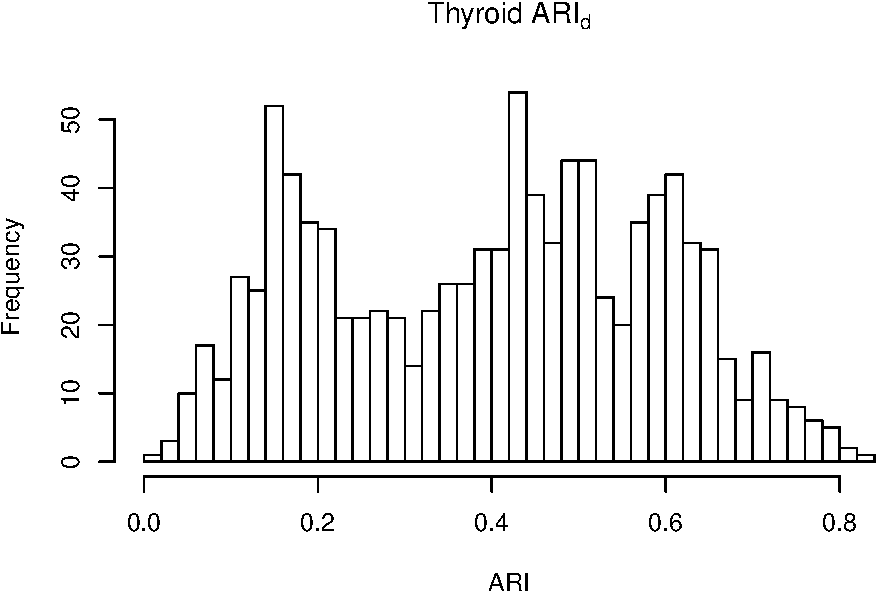
\includegraphics[width=1\linewidth]{Report_files/figure-latex/unnamed-chunk-3-1} \end{center}

\begin{center}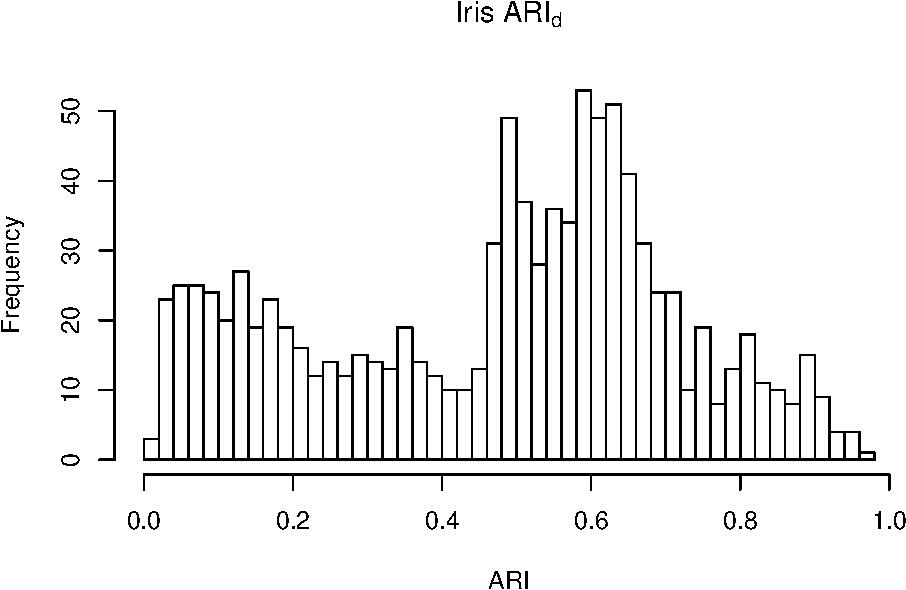
\includegraphics[width=1\linewidth]{Report_files/figure-latex/unnamed-chunk-3-2} \end{center}

\begin{center}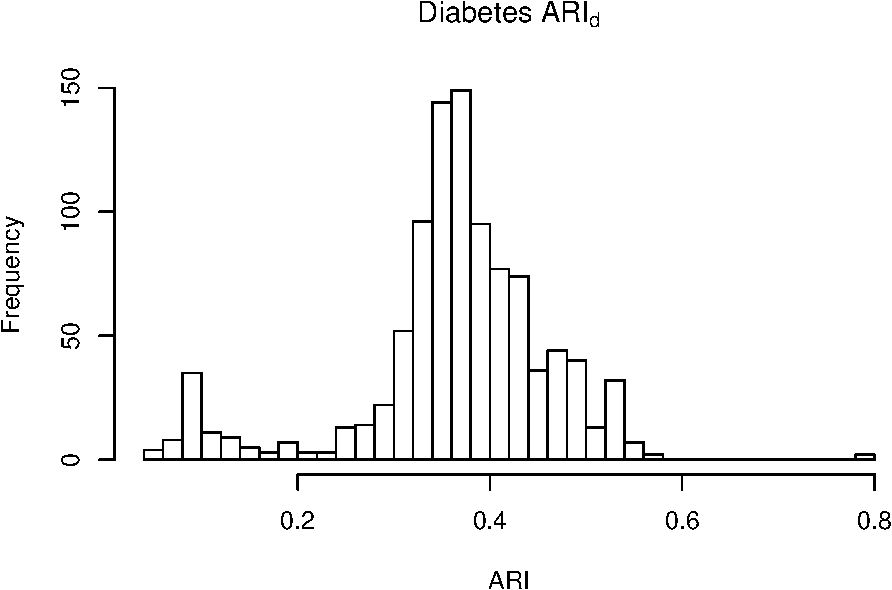
\includegraphics[width=1\linewidth]{Report_files/figure-latex/unnamed-chunk-3-3} \end{center}

\begin{center}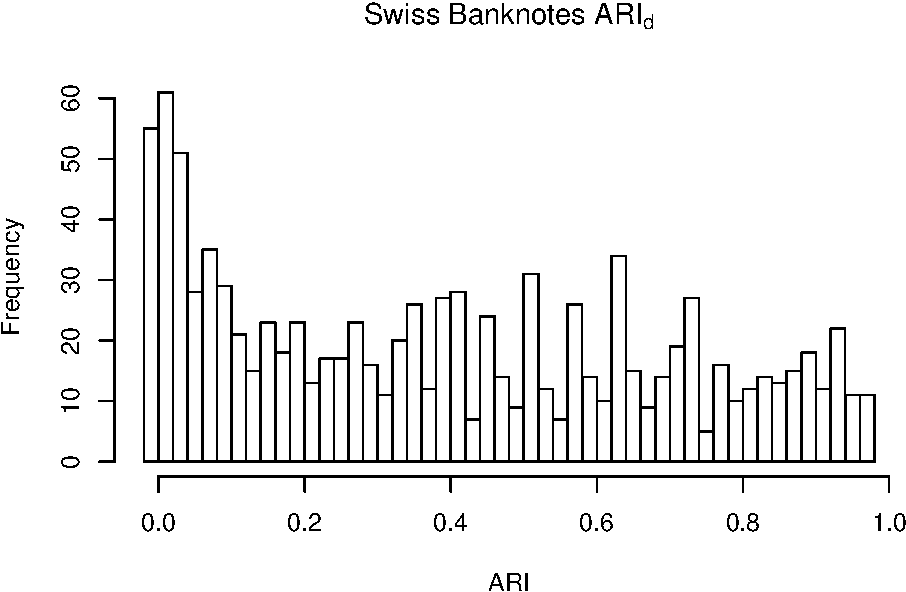
\includegraphics[width=1\linewidth]{Report_files/figure-latex/unnamed-chunk-3-4} \end{center}

\begin{center}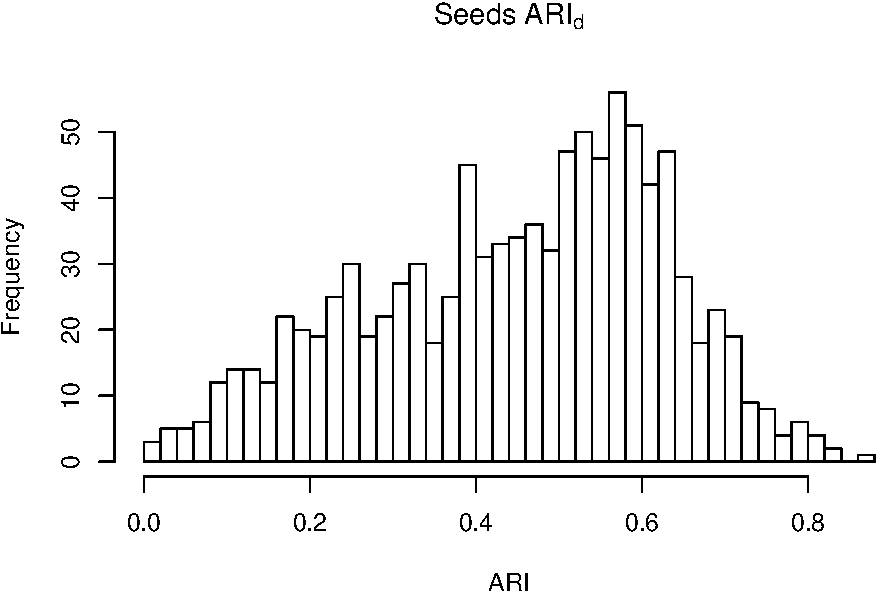
\includegraphics[width=1\linewidth]{Report_files/figure-latex/unnamed-chunk-3-5} \end{center}

\begin{center}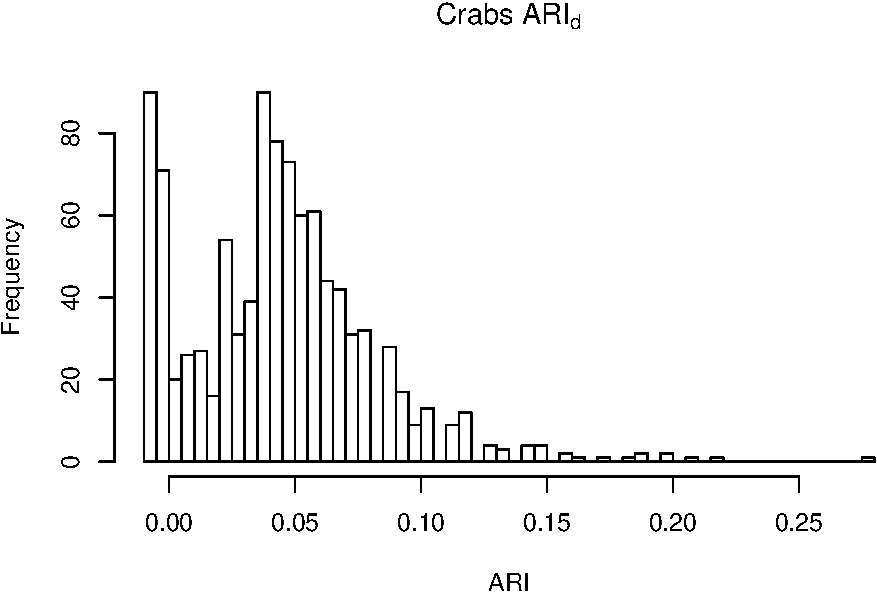
\includegraphics[width=1\linewidth]{Report_files/figure-latex/unnamed-chunk-3-6} \end{center}

\begin{center}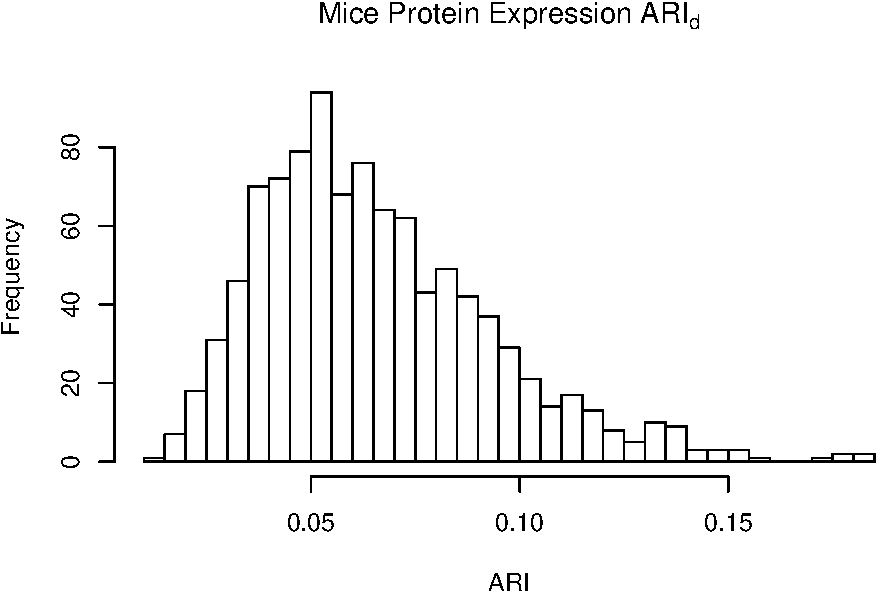
\includegraphics[width=1\linewidth]{Report_files/figure-latex/unnamed-chunk-3-7} \end{center}

\section{\texorpdfstring{For \(\alpha\) = 2, p(reduced dimention) =
3}{For \textbackslash{}alpha = 2, p(reduced dimention) = 3}}\label{for-alpha-2-preduced-dimention-3}

\subsection{Tabel}\label{tabel}

\begin{table}[H]
\centering\rowcolors{2}{gray!6}{white}

\begin{tabular}{lrrr}
\hiderowcolors
\toprule
Dataset & ARI\_d & ARI\_p & C\_e\\
\midrule
\showrowcolors
Thyroid & 0.5831656 & 0.4344288 & 15\\
Iris & 0.6201352 & 0.5359746 & 8\\
Diabetes & 0.3801662 & 0.3805076 & 0\\
Swiss Banknotes & 0.8456292 & 0.4714675 & 37\\
Seeds & 0.7732937 & 0.5299329 & 24\\
\addlinespace
Mice Protein Expression & 0.1316575 & 0.0814613 & 5\\
Crabs & 0.0481402 & 0.0485252 & 0\\
\bottomrule
\end{tabular}
\rowcolors{2}{white}{white}
\end{table}

\subsection{Histograms}\label{histograms-1}

\begin{center}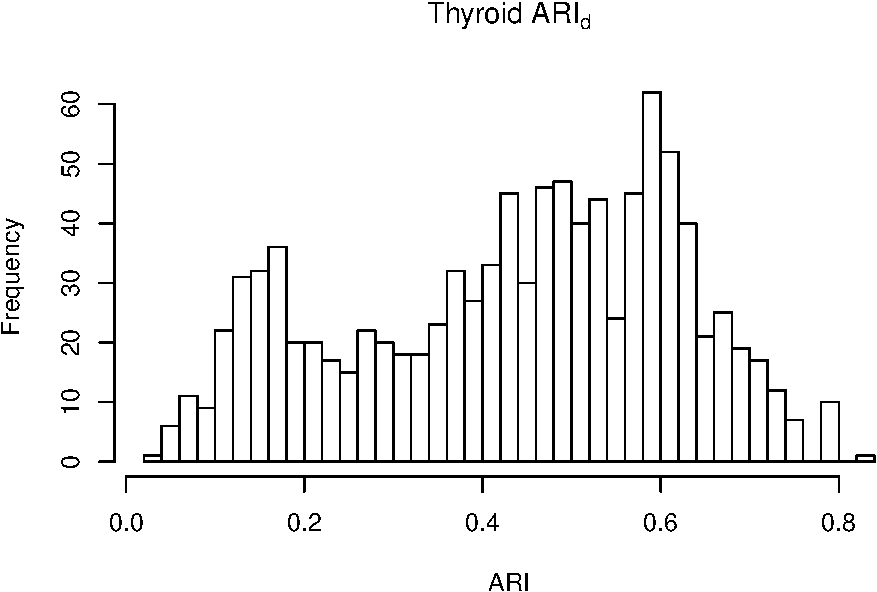
\includegraphics[width=1\linewidth]{Report_files/figure-latex/unnamed-chunk-6-1} \end{center}

\begin{center}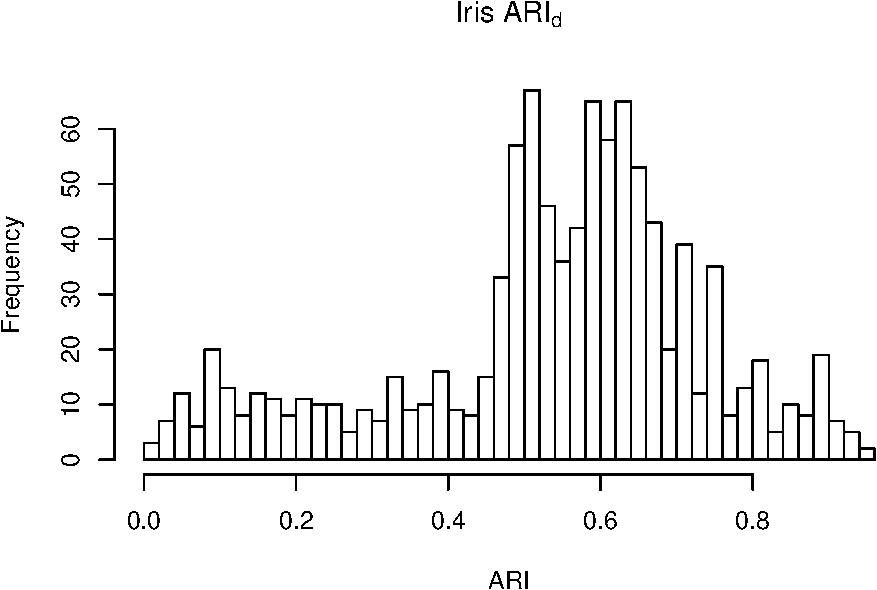
\includegraphics[width=1\linewidth]{Report_files/figure-latex/unnamed-chunk-6-2} \end{center}

\begin{center}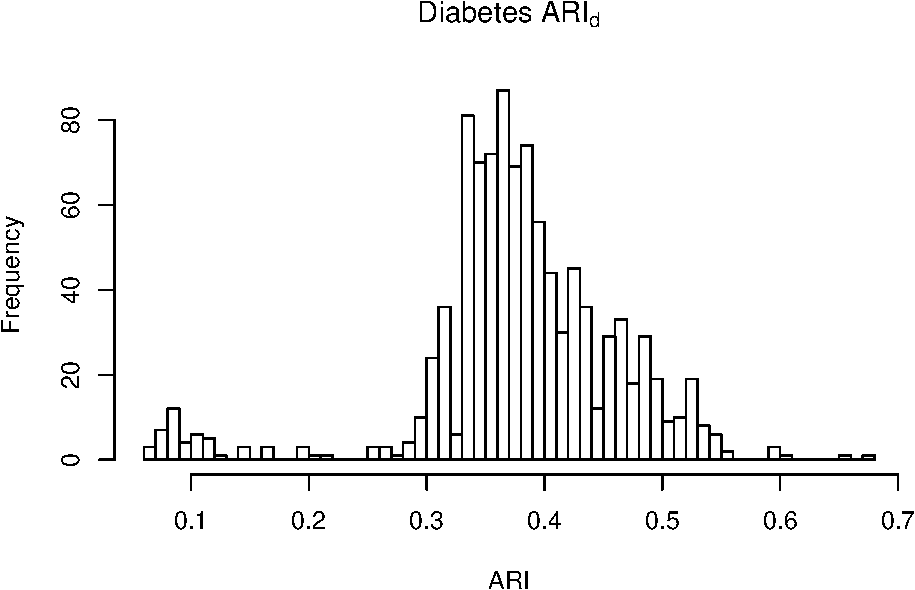
\includegraphics[width=1\linewidth]{Report_files/figure-latex/unnamed-chunk-6-3} \end{center}

\begin{center}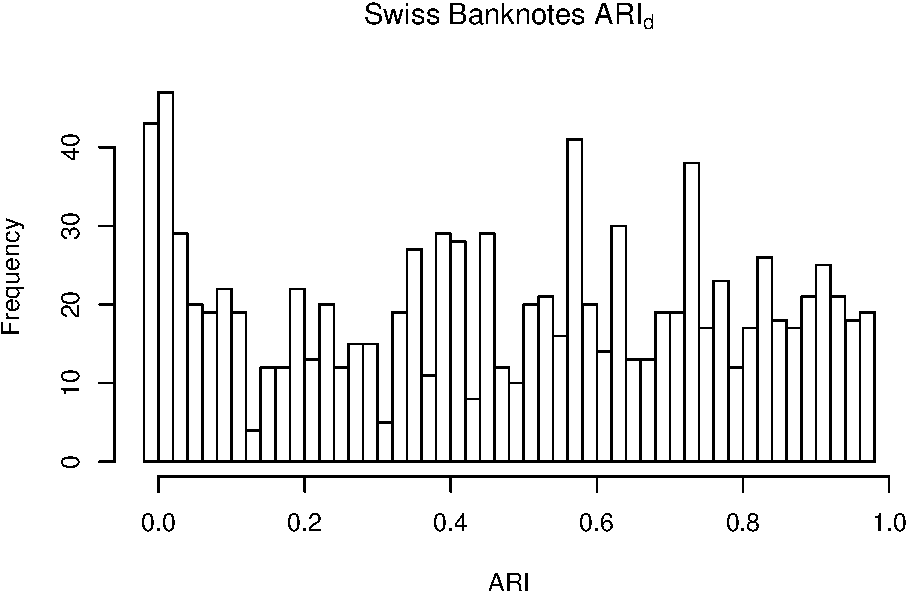
\includegraphics[width=1\linewidth]{Report_files/figure-latex/unnamed-chunk-6-4} \end{center}

\begin{center}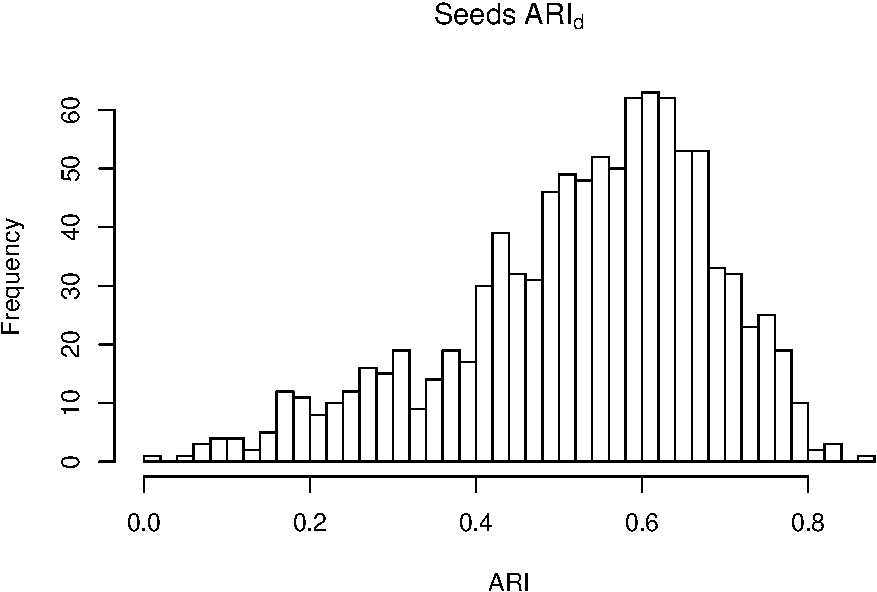
\includegraphics[width=1\linewidth]{Report_files/figure-latex/unnamed-chunk-6-5} \end{center}

\begin{center}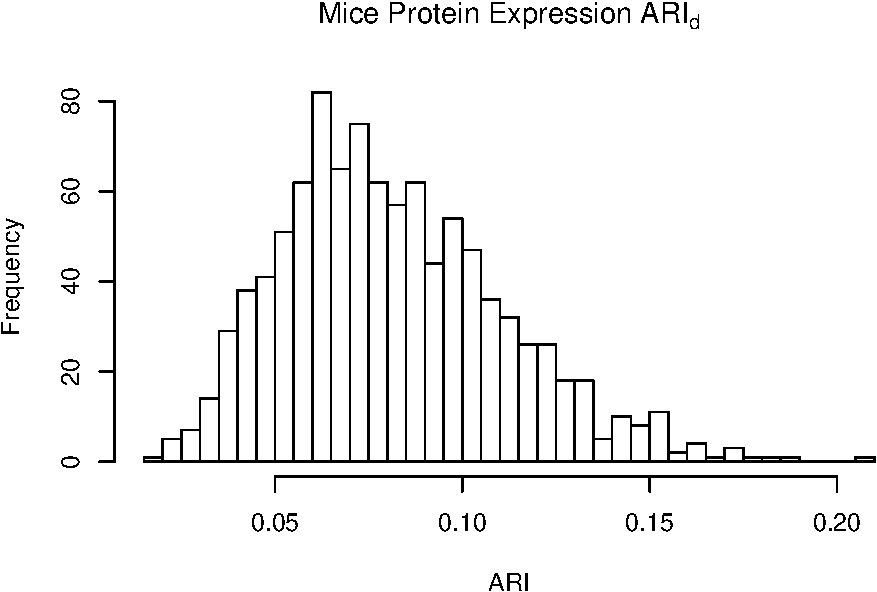
\includegraphics[width=1\linewidth]{Report_files/figure-latex/unnamed-chunk-6-6} \end{center}

\begin{center}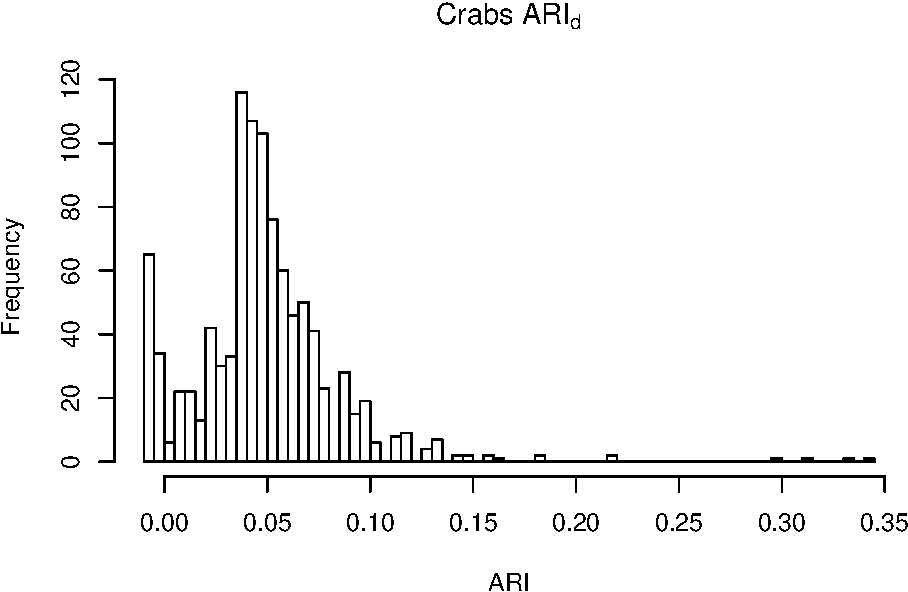
\includegraphics[width=1\linewidth]{Report_files/figure-latex/unnamed-chunk-6-7} \end{center}

\section{\texorpdfstring{For \(\alpha\) = 1, p(reduced dimention) =
2}{For \textbackslash{}alpha = 1, p(reduced dimention) = 2}}\label{for-alpha-1-preduced-dimention-2}

\subsection{Tabel}\label{tabel-1}

\begin{table}[H]
\centering\rowcolors{2}{gray!6}{white}

\begin{tabular}{lrrr}
\hiderowcolors
\toprule
Dataset & ARI\_d & ARI\_p & C\_e\\
\midrule
\showrowcolors
Thyroid & 0.5831656 & 0.3559301 & 23\\
Iris & 0.6201352 & 0.5078172 & 11\\
Diabetes & 0.3801662 & 0.3341399 & 5\\
Swiss Banknotes & 0.8456292 & 0.4011119 & 44\\
Seeds & 0.7732937 & 0.4488349 & 32\\
\addlinespace
Mice Protein Expression & 0.1317342 & 0.0592468 & 7\\
Crabs & 0.0481402 & 0.0469365 & 0\\
\bottomrule
\end{tabular}
\rowcolors{2}{white}{white}
\end{table}

\subsection{Histograms}\label{histograms-2}

\begin{center}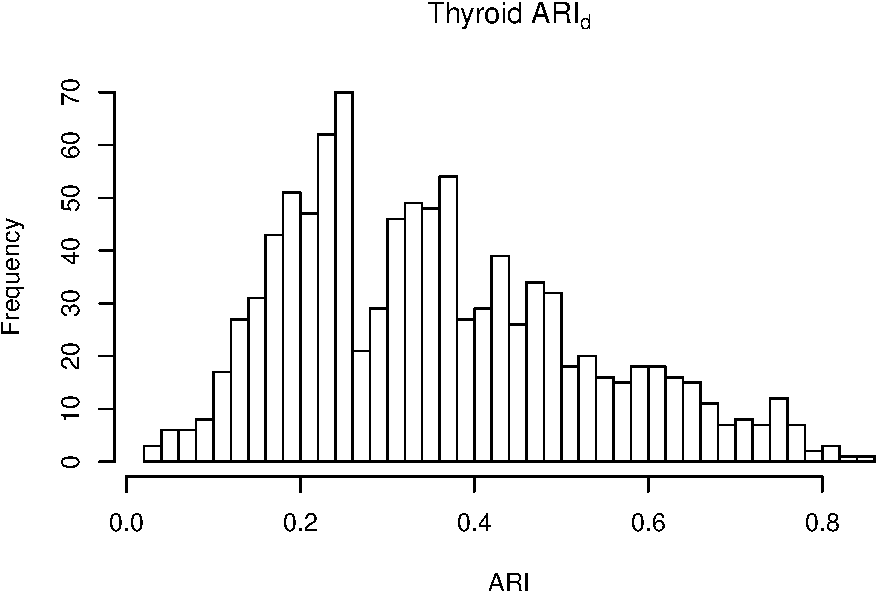
\includegraphics[width=1\linewidth]{Report_files/figure-latex/unnamed-chunk-9-1} \end{center}

\begin{center}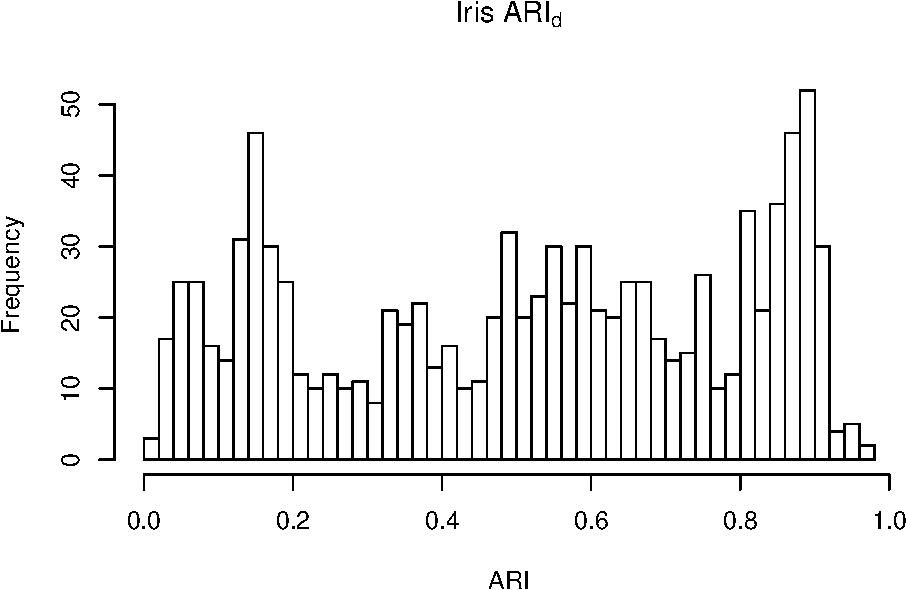
\includegraphics[width=1\linewidth]{Report_files/figure-latex/unnamed-chunk-9-2} \end{center}

\begin{center}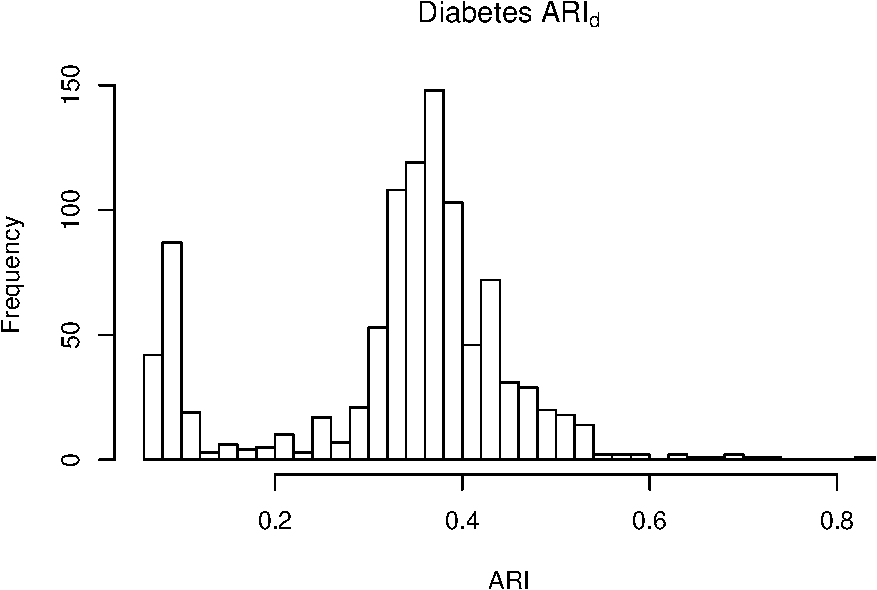
\includegraphics[width=1\linewidth]{Report_files/figure-latex/unnamed-chunk-9-3} \end{center}

\begin{center}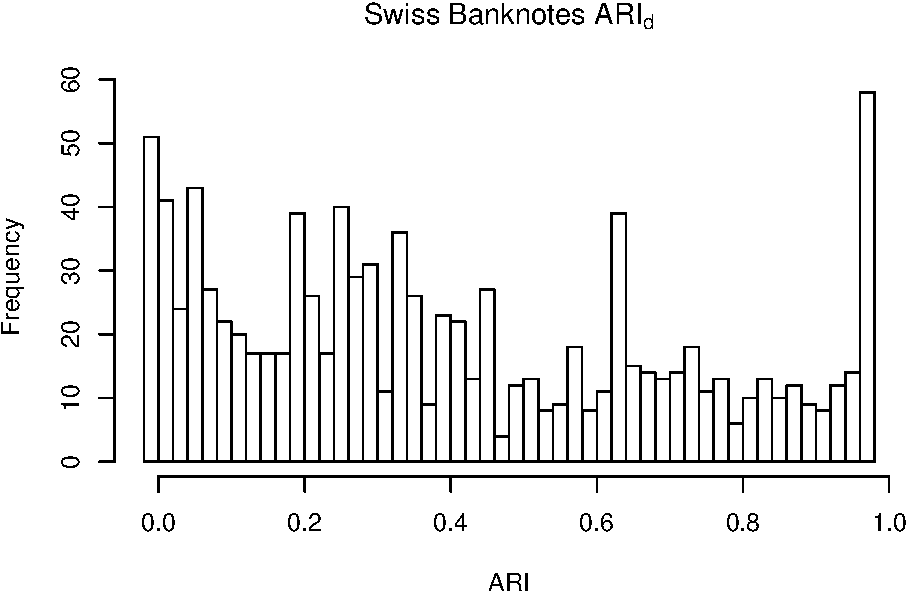
\includegraphics[width=1\linewidth]{Report_files/figure-latex/unnamed-chunk-9-4} \end{center}

\begin{center}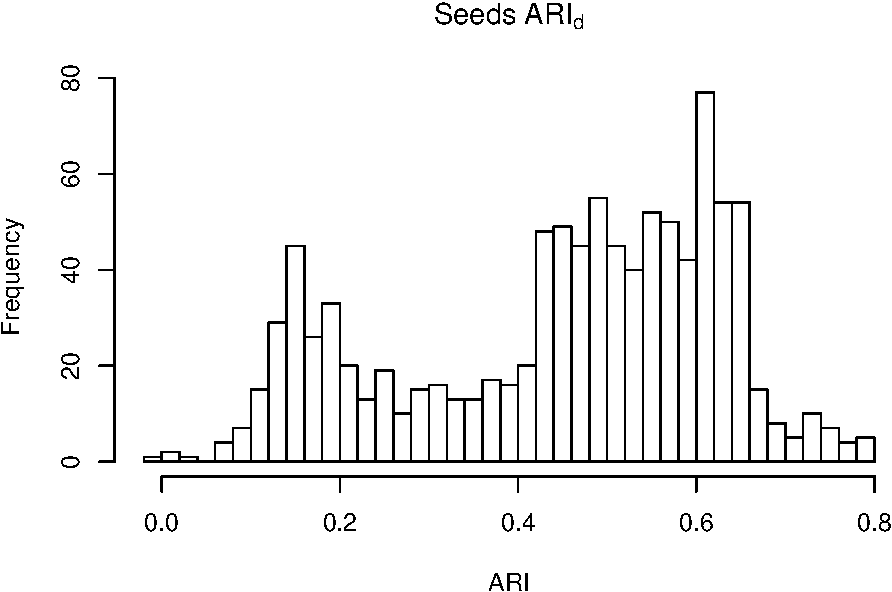
\includegraphics[width=1\linewidth]{Report_files/figure-latex/unnamed-chunk-9-5} \end{center}

\begin{center}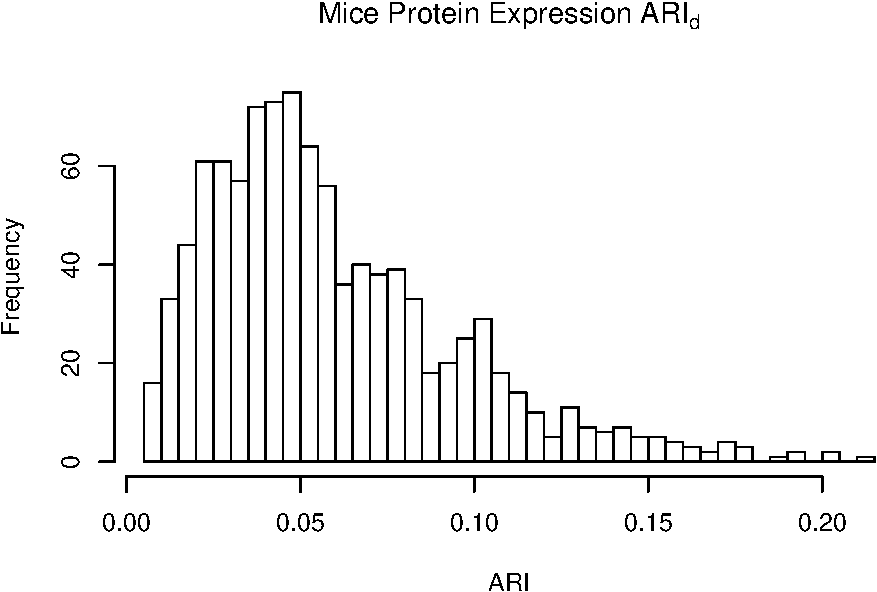
\includegraphics[width=1\linewidth]{Report_files/figure-latex/unnamed-chunk-9-6} \end{center}

\begin{center}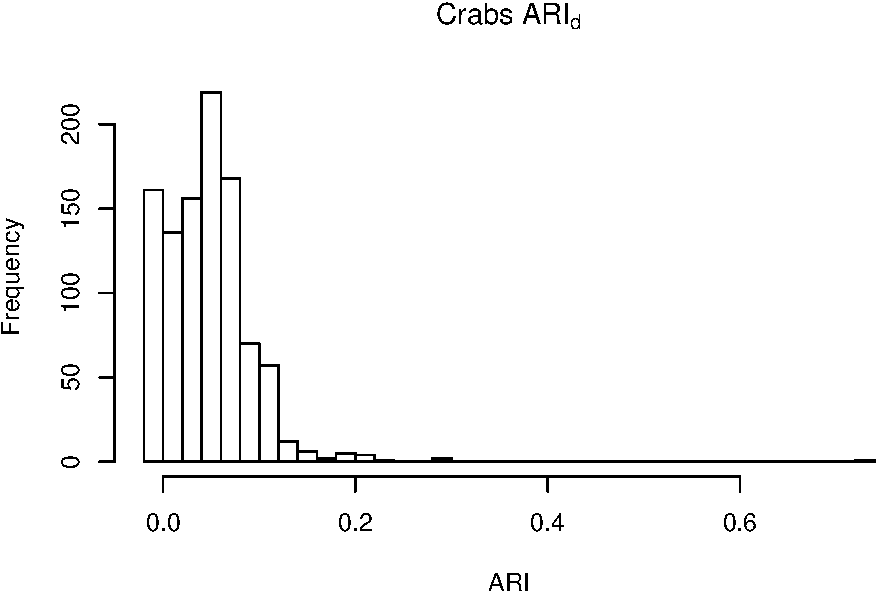
\includegraphics[width=1\linewidth]{Report_files/figure-latex/unnamed-chunk-9-7} \end{center}

\section{\texorpdfstring{For \(\alpha\) = 1, p(reduced dimention) =
3}{For \textbackslash{}alpha = 1, p(reduced dimention) = 3}}\label{for-alpha-1-preduced-dimention-3}

\subsection{Tabel}\label{tabel-2}

\begin{table}[H]
\centering\rowcolors{2}{gray!6}{white}

\begin{tabular}{lrrr}
\hiderowcolors
\toprule
Dataset & ARI\_d & ARI\_p & C\_e\\
\midrule
\showrowcolors
Thyroid & 0.5831656 & 0.3658900 & 22\\
Iris & 0.6201352 & 0.5441285 & 8\\
Diabetes & 0.3801662 & 0.3460760 & 3\\
Swiss Banknotes & 0.8456292 & 0.4330544 & 41\\
Seeds & 0.7732937 & 0.4697687 & 30\\
\addlinespace
Mice Protein Expression & 0.1317362 & 0.0659775 & 7\\
Crabs & 0.0481402 & 0.0452313 & 0\\
\bottomrule
\end{tabular}
\rowcolors{2}{white}{white}
\end{table}

\subsection{Histograms}\label{histograms-3}

\begin{center}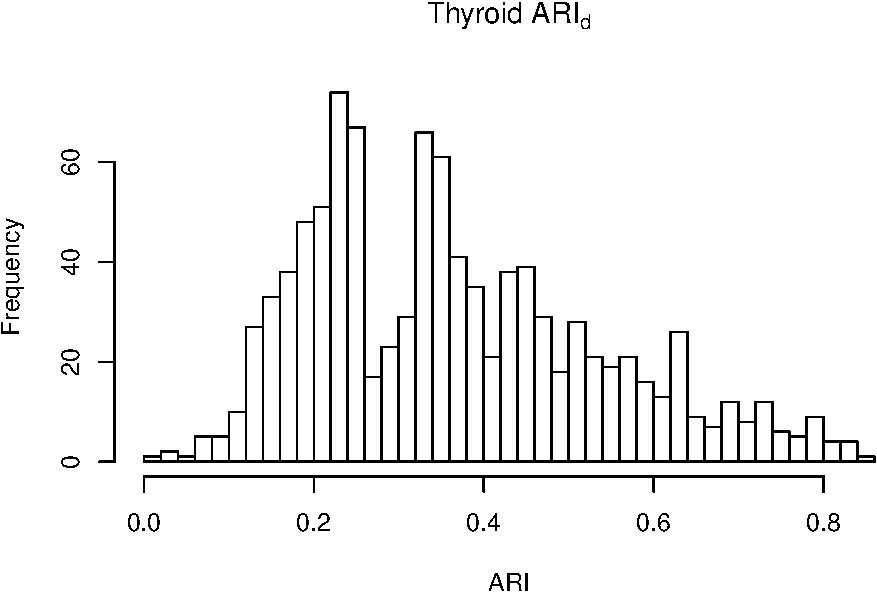
\includegraphics[width=1\linewidth]{Report_files/figure-latex/unnamed-chunk-12-1} \end{center}

\begin{center}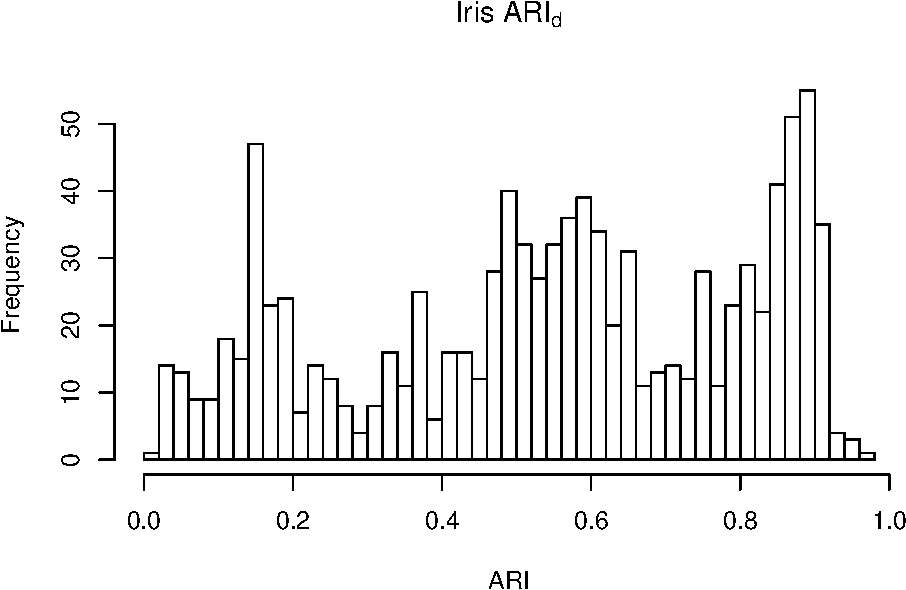
\includegraphics[width=1\linewidth]{Report_files/figure-latex/unnamed-chunk-12-2} \end{center}

\begin{center}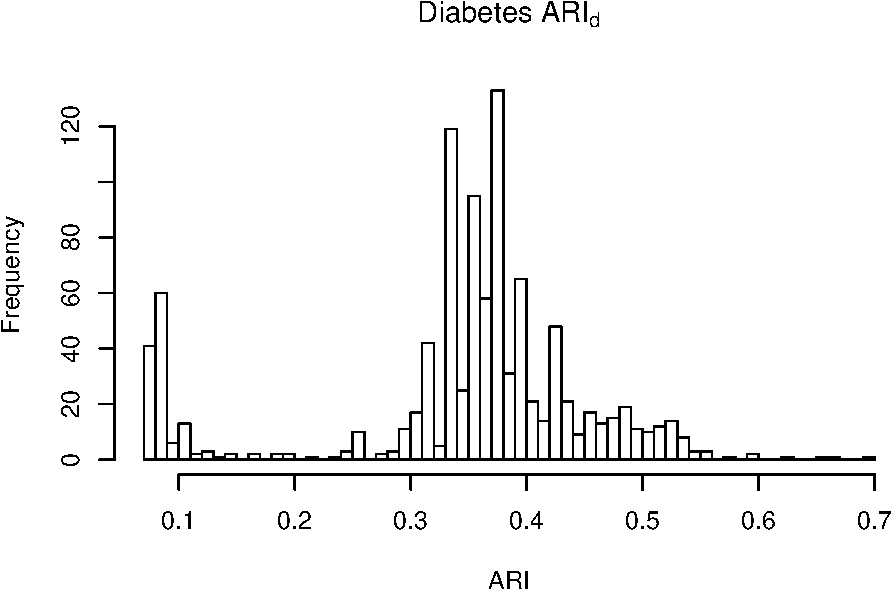
\includegraphics[width=1\linewidth]{Report_files/figure-latex/unnamed-chunk-12-3} \end{center}

\begin{center}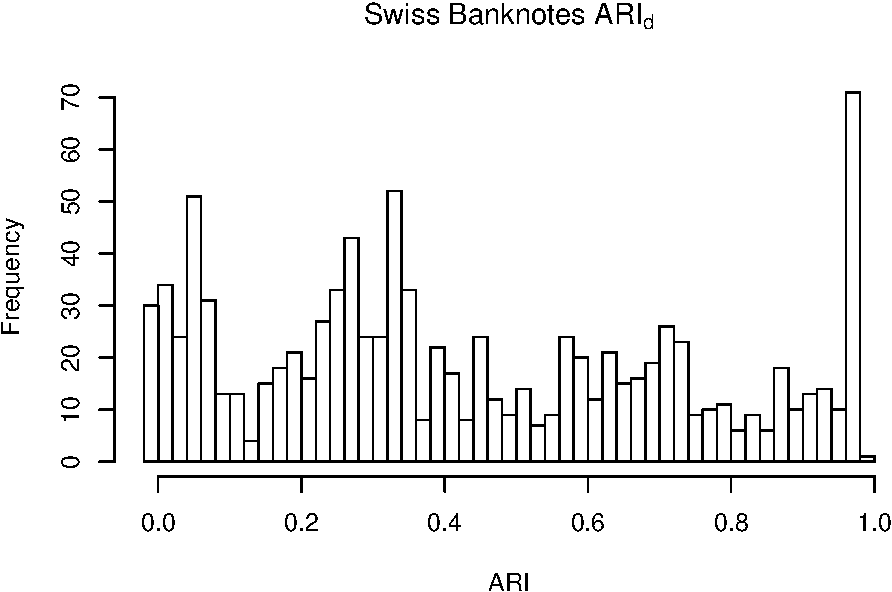
\includegraphics[width=1\linewidth]{Report_files/figure-latex/unnamed-chunk-12-4} \end{center}

\begin{center}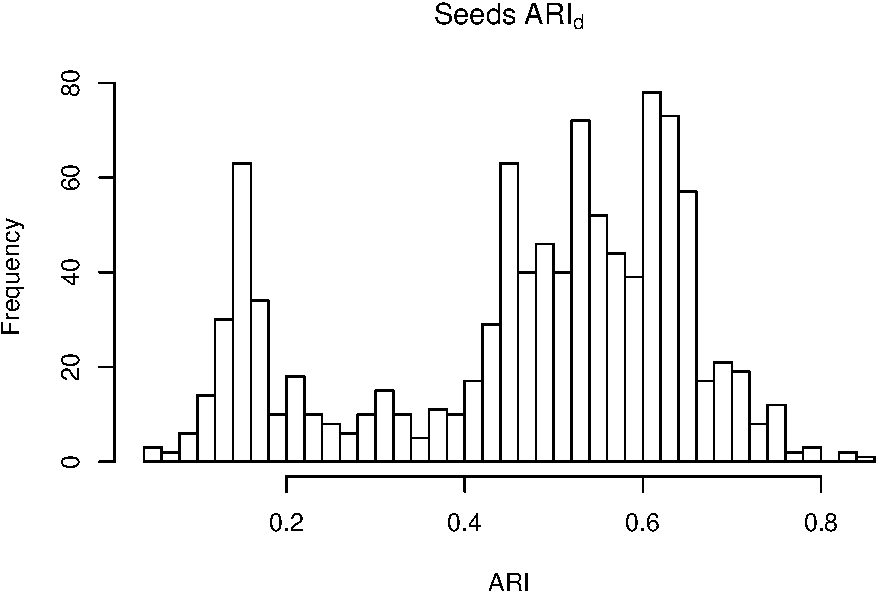
\includegraphics[width=1\linewidth]{Report_files/figure-latex/unnamed-chunk-12-5} \end{center}

\begin{center}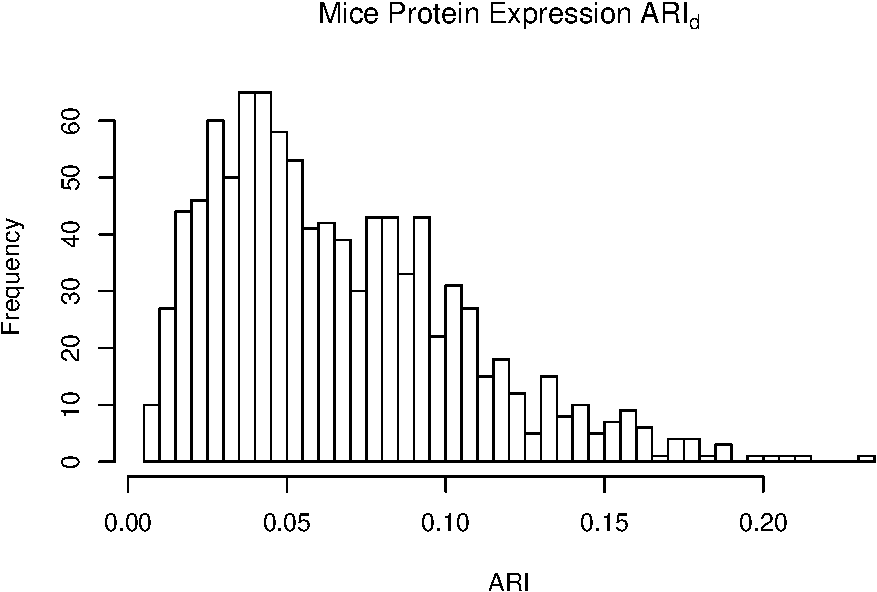
\includegraphics[width=1\linewidth]{Report_files/figure-latex/unnamed-chunk-12-6} \end{center}

\begin{center}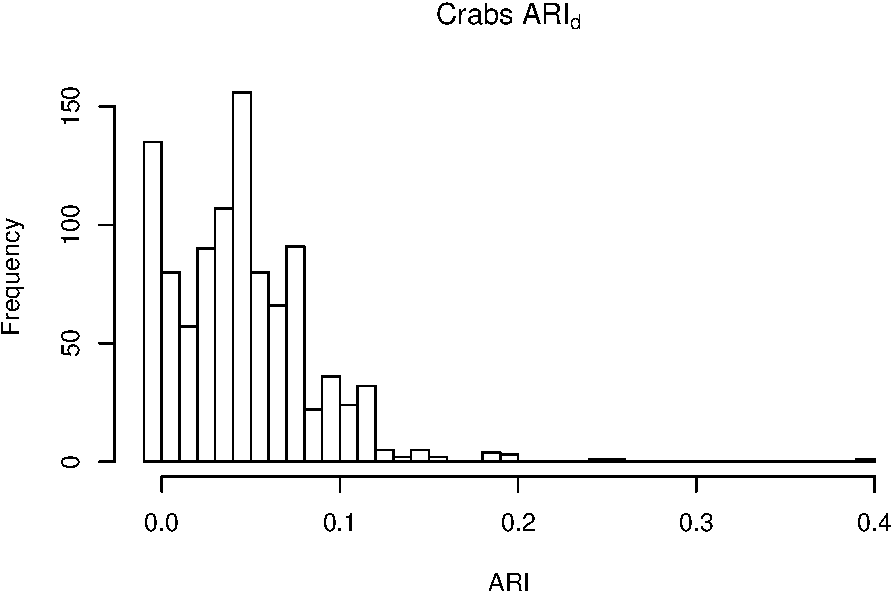
\includegraphics[width=1\linewidth]{Report_files/figure-latex/unnamed-chunk-12-7} \end{center}

\end{latin}


%--------------------------------------------------------------------------appendix( مراجع و پیوست ها)
\chapterfont{\vspace*{-2em}\centering\LARGE}%

\appendix
\bibliographystyle{plain-fa}
\bibliography{references}
\chapter*{‌پیوست}
\markboth{پیوست}{}
\addcontentsline{toc}{chapter}{پیوست}

\section*{
کد دریافت داده‌ها }
\begin{latin}
\begin{Verbatim}[breaklines=true, breakanywhere=true, baselinestretch=1]

rm(list = ls(all.names = TRUE))
library(beepr)

library(rgl)
library(stabledist)
library(MASS)
library(mclust)
library(xlsx)

if(file.exists('data.RData')) {
  load(file = 'data.RData')
} else {

crabs <- crabs #MASS
data("diabetes") #mclust
data("thyroid") #mclust
data("banknote") #mclust

irisUci <- read.csv('https://archive.ics.uci.edu/ml/machine-learning-databases/iris/iris.data', header = FALSE)
names(irisUci) <- names(iris)
seeds <- read.table('https://archive.ics.uci.edu/ml/machine-learning-databases/00236/seeds_dataset.txt', header = FALSE)

tmpFile <- tempfile(fileext = '.xls')
download.file('https://archive.ics.uci.edu/ml/machine-learning-databases/00342/Data_Cortex_Nuclear.xls', destfile = tmpFile)
MPE <- read.xlsx(tmpFile, sheetIndex = 1)

rm(tmpFile)

save(list = ls(), file = 'data.RData')

}

beep(4)


\end{Verbatim}
\end{latin}

‍\section*{
کد مرتب سازی داده‌ها }
\begin{latin}
\begin{Verbatim}[breaklines=true, breakanywhere=true, baselinestretch=1]

library(tictoc)
source('Util.R')
d <- list()
apply(thyroid, 2, function(x) {sum(is.na(x) | is.null(x))})
d$thyroid$data <- thyroid[,2:6]
d$thyroid$class <- as.numeric(thyroid$Diagnosis)
d$thyroid$data <- normalizeData(d$thyroid$data)
d$thyroid$name <- 'Thyroid'

apply(irisUci, 2, function(x) {sum(is.na(x) | is.null(x))})
d$iris$data <- irisUci[,1:4]
d$iris$class <- as.numeric(irisUci$Species)
d$iris$data <- normalizeData(d$iris$data)
d$iris$name <- 'Iris'

apply(diabetes, 2, function(x) {sum(is.na(x) | is.null(x))})
d$diabetes$data <- diabetes[,2:4]
d$diabetes$class <- as.numeric(diabetes$class)
d$diabetes$data <- normalizeData(d$diabetes$data)
d$diabetes$name <- 'Diabetes'

apply(banknote, 2, function(x) {sum(is.na(x) | is.null(x))})
d$banknote$data <- banknote[,2:7]
d$banknote$class <- as.numeric(banknote$Status)
d$banknote$data <- normalizeData(d$banknote$data)
d$banknote$name <- 'Swiss Banknotes'

apply(seeds, 2, function(x) {sum(is.na(x) | is.null(x))})
d$seeds$data <- seeds[,1:7]
d$seeds$class <- as.numeric(seeds[,8])
d$seeds$data <- normalizeData(d$seeds$data)
d$seeds$name <- 'Seeds'

apply(MPE, 2, function(x) {sum(is.na(x) | is.null(x))})
MPEwoNA <- MPE
MPEwoNA[,2:78] <- apply(MPE[,2:78], 2, function(x) { x[is.na(x)] <- mean(x, na.rm = TRUE); x } ) 
apply(MPEwoNA, 2, function(x) {sum(is.na(x) | is.null(x))})
d$MPEwoNA$data <- MPEwoNA[,2:78]
d$MPEwoNA$class <- as.numeric(MPEwoNA$class)
d$MPEwoNA$data <- normalizeData(d$MPEwoNA$data)
d$MPEwoNA$name <- 'Mice Protein Expression'

apply(crabs, 2, function(x) {sum(is.na(x) | is.null(x))})
d$crabs$data <- crabs[,4:8]
d$crabs$data <- cbind(d$crabs$data, as.numeric(crabs[,2]))
d$crabs$class <- as.numeric(crabs[,1])
d$crabs$data <- normalizeData(d$crabs$data)
d$crabs$name <- 'Crabs'

\end{Verbatim}
\end{latin}

\section*{
کد توابع مورد استفاده داده‌ها }
\begin{latin}
\begin{Verbatim}[breaklines=true, breakanywhere=true, baselinestretch=1]

# Sample Data Generation Functions ----------------------------------------

# _Univariate Normal ------------------------------------------------------

sampleDataUniNormal <- function(cf) {
  
  out <- dataConfiguration(cf)
  
  cf <- out$cf
  dClass <- out$dClass
  dClassMean <- out$dClassMean
  dClassVar <- out$dClassVar
  
  d <- matrix(rnorm(cf$nSample * cf$nDimention), nrow = cf$nSample)
  
  for(i in 1:cf$nClass) {
    for(j in 1:cf$nDimention) {
      d[(cf$classIndex[i]+1):cf$classIndex[i+1], j] <-
        sqrt(dClassVar[i, j, j]) * d[(cf$classIndex[i]+1):cf$classIndex[i+1], j]
    }
    d[(cf$classIndex[i]+1):cf$classIndex[i+1], ] <- 
      d[(cf$classIndex[i]+1):cf$classIndex[i+1], ] +
      matrix(rep(dClassMean[i,], cf$classIndex[i+1] - cf$classIndex[i]), 
             ncol = cf$nDimention,
             byrow = TRUE)
  }
  
  permuteIndex <- sample.int(cf$nSample, size = cf$nSample)
  d <- d[permuteIndex, ]
  dClass <- dClass[permuteIndex]
  
  return(list(data = d, class = dClass))
  
}

if(FALSE) {
  d <- sampleDataUniNormal(cf)
  print(head(data.frame(d = d$data, class = d$class)))
  plot(d$data, type = 'p', col = d$class, asp = 1)
  plot3d(d$data, col = d$class, size = 2, type = 's')
  aspect3d(x = 'iso')
}

# _Multivariate Normal ----------------------------------------------------

sampleDataMultiNormal <- function(cf) {
  out <- dataConfiguration(cf, multiVariate = TRUE)
  
  cf <- out$cf
  dClass <- out$dClass
  dClassMean <- out$dClassMean
  dClassVar <- out$dClassVar
  
  d <- matrix(0, nrow = 0, ncol = cf$nDimention)
  
  for(i in 1:cf$nClass) {
    d <- rbind(d, mvrnorm(cf$classIndex[i+1] - cf$classIndex[i],
                          mu = out$dClassMean[i,], Sigma = out$dClassVar[i, , ])
    )
  }
  
  permuteIndex <- sample.int(cf$nSample, size = cf$nSample)
  d <- d[permuteIndex, ]
  dClass <- dClass[permuteIndex]
  
  return(list(data = d, class = dClass))
  
}

if(FALSE) {
  d <- sampleDataMultiNormal(cf)
  print(head(data.frame(d = d$data, class = d$class)))
  plot(d$data, type = 'p', col = d$class, asp = 1)
  plot3d(d$data, col = d$class, size = 2, type = 's')
  aspect3d(x = 'iso')
}

# _Alpha Univariate -------------------------------------------------------

sampleDataUniStable <- function(cf, alpha) {
  
  out <- dataConfiguration(cf)
  
  cf <- out$cf
  dClass <- out$dClass
  dClassMean <- out$dClassMean
  dClassVar <- out$dClassVar
  
  d <- matrix(rstable(cf$nSample * cf$nDimention, alpha = alpha, beta = 0),
              nrow = cf$nSample)
  
  for(i in 1:cf$nClass) {
    for(j in 1:cf$nDimention) {
      d[(cf$classIndex[i]+1):cf$classIndex[i+1], j] <-
        sqrt(dClassVar[i, j, j]) * d[(cf$classIndex[i]+1):cf$classIndex[i+1], j]
    }
    d[(cf$classIndex[i]+1):cf$classIndex[i+1], ] <- 
      d[(cf$classIndex[i]+1):cf$classIndex[i+1], ] +
      matrix(rep(dClassMean[i,], cf$classIndex[i+1] - cf$classIndex[i]), 
             ncol = cf$nDimention,
             byrow = TRUE)
  }
  
  permuteIndex <- sample.int(cf$nSample, size = cf$nSample)
  d <- d[permuteIndex, ]
  dClass <- dClass[permuteIndex]
  
  return(list(data = d, class = dClass))
  
}

if(FALSE) {
  d <- sampleDataUniStable(cf, 1.8)
  print(head(data.frame(d = d$data, class = d$class)))
  plot(d$data, type = 'p', col = d$class, asp = 1)
  plot3d(d$data, col = d$class, size = 2, type = 's')
  aspect3d(x = 'iso')
}

# _Alpha Multivariate -----------------------------------------------------

sampleDataMultiStable <- function(cf, alpha) {
  
  out <- dataConfiguration(cf)
  
  cf <- out$cf
  dClass <- out$dClass
  dClassMean <- out$dClassMean
  dClassVar <- out$dClassVar
  
  cf$nDimention <- 2
  
  theta <- c(0, pi/4, pi/2, 3 * pi / 4)
  weight <- c(1,2,1,1)
  
  d <- 
    matrix(
      rstable(cf$nSample * length(theta), alpha = alpha, beta = 0),
      ncol = length(theta)
    ) %*%
    matrix(
      c(
        (cos(theta) * weight) / sum(abs(cos(theta) * weight)),
        (sin(theta) * weight) / sum(abs(sin(theta) * weight))
      ),
      ncol = cf$nDimention
    )
  
  for(i in 1:cf$nClass) {
    d[(cf$classIndex[i]+1):cf$classIndex[i+1], ] <- 
      d[(cf$classIndex[i]+1):cf$classIndex[i+1], ] +
      matrix(rep(dClassMean[i,], cf$classIndex[i+1] - cf$classIndex[i]), 
             ncol = cf$nDimention,
             byrow = TRUE)
  }
  
  permuteIndex <- sample.int(cf$nSample, size = cf$nSample)
  d <- d[permuteIndex, ]
  dClass <- dClass[permuteIndex]
  
  return(list(data = d, class = dClass))
  
}

if(FALSE) {
  d <- sampleDataMultiStable(cf, 1.8)
  print(head(data.frame(d = d$data, class = d$class)))
  plot(d$data, type = 'p', col = d$class, asp = 1)
  plot3d(d$data, col = d$class, size = 2, type = 's')
  aspect3d(x = 'iso')
}




# Dimention Reduction -----------------------------------------------------

randomProjection <- function(d, targetNumDimention, alpha = 2) {
  
  pm <- matrix(rstable(ncol(d) * targetNumDimention, alpha = alpha, beta = 0),
               nrow = ncol(d))
  
  d %*% pm
  
}

sRandomProjection <- function(d, targetNumDimention, s = 2) {
  
  r <- runif(ncol(d) * targetNumDimention, min = 0, max = 2*s)
  r[r <= 1] = -1
  r[r >= (2*s-1)] = 1
  r[r != 1 & r != -1] <- 0
  pm <- matrix(r,
               nrow = ncol(d))
  
  d %*% pm
  
}



# Util Functions ----------------------------------------------------------

dataConfiguration <- function(cf, multiVariate = FALSE) {
  
  if(!('classIndex' %in% names(cf))) {
    if(!('classRatio' %in% names(cf))) {
      cf$classRatio <- rep(1/cf$nClass, cf$nClass)
    }
    cf$classIndex <- c(0, round( cumsum(cf$classRatio) * cf$nSample))
  }
  
  # dClass <- rep(0, cf$nSample)
  dClass <- integer(0)
  for(i in 1:cf$nClass) {
    dClass <- c(dClass, rep(i, cf$classIndex[i+1]- cf$classIndex[i]))
  }
  
  dClassMean <- matrix(0, nrow = cf$nClass, ncol = cf$nDimention  ,byrow = TRUE)
  theta <- 2 * pi / cf$nClass
  radious <- 5
  for(i in 1:cf$nClass) {
    dClassMean[i, 1] <- radious * cos(theta * i)
    dClassMean[i, 2] <- radious * sin(theta * i)
  }
  # dClassMean[ ,1] <- 10 * seq(0, cf$nClass-1)
  
  dClassVar <- array(0, dim = c(cf$nClass, cf$nDimention, cf$nDimention))
  if(multiVariate) {
    for(i in 1:cf$nClass) {
      dClassVar[i, , ] <- randCovMat(cf$nDimention)
    }
  } else {
    for(i in 1:cf$nClass) {
      dClassVar[i, , ] <- diag(cf$nDimention)
    }
  }
  
  return(list(
    cf = cf,
    dClass = dClass,
    dClassMean = dClassMean,
    dClassVar = dClassVar
  ))
  
}

randCovMat <- function(nd, sdev = NULL) {

  if (is.null(sdev)) {
    sdev <- rep(1, nd)
  }
  out <- diag(nd)
  index <- data.frame(n = 1:((nd*(nd-1)) / 2))
  index$i <- ceiling((-1+sqrt(1+8*index$n)) / 2)
  index$j <- index$n - ((index$i - 1)^2 + (index$i - 1)) / 2
  index$i <- index$i + 1
  index <- index[sample(index$n, nrow(index)), ]
  
  for(i in 1:nrow(index)) {
    candidate <- seq(from = -1, to = 1, by = 0.01)
    candidate <- sample(candidate, size = length(candidate))
    for(k in 1:length(candidate)) {
      out[index$i[i],index$j[i]] <- candidate[k]
      out[index$j[i],index$i[i]] <- out[index$i[i],index$j[i]]
      if(det(out) > 0) break
    } 
  }
  msdev <- diag(nd) * sdev
  out <- msdev %*% out %*% msdev
}

normalizeData <- function(d) {
  d <- apply(d, 2, function(x) {(x-mean(x))/sd(x)})
  d
}

ARIreport <- function(d, tDimention = 2, alpha = 2) {
  
  nClass <- length(unique(d$class))
  
  cl <- kmeans(d$data, nClass, nstart = 20, iter.max = 100)
  ari_d <- (adjustedRandIndex(d$class, cl$cluster))
  
  d$pdata <- randomProjection(d$data, tDimention, alpha = alpha)
  clp <- kmeans(d$pdata, nClass, nstart = 20, iter.max = 100)
  ari_p <- (adjustedRandIndex(d$class, clp$cluster))
  
  c_e <- 100 * (ari_d - ari_p)
  
  data.frame(ari_d = ari_d, ari_p = ari_p, c_e = c_e)
}

ARIreport_s <- function(d, tDimention = 2, s = 2) {
  
  nClass <- length(unique(d$class))
  
  cl <- kmeans(d$data, nClass, nstart = 20, iter.max = 100)
  ari_d <- (adjustedRandIndex(d$class, cl$cluster))
  
  check <- TRUE
  while(check){
    check <- tryCatch({
      d$pdata <- sRandomProjection(d$data, tDimention, s = s)
      clp <- kmeans(d$pdata, nClass, nstart = 20, iter.max = 100)
      FALSE
      }, error = function(e) {print('not enough distinct points'); TRUE})
  }
  
  ari_p <- (adjustedRandIndex(d$class, clp$cluster))
  
  c_e <- 100 * (ari_d - ari_p)
  
  data.frame(ari_d = ari_d, ari_p = ari_p, c_e = c_e)
}

\end{Verbatim}
\end{latin}


\section*{
کد گزارش‌گیری }
\begin{latin}
\begin{Verbatim}[breaklines=true, breakanywhere=true, baselinestretch=1]

iterations <- 1000
tic()
for(dIndex in names(d)) {
  out <- data.frame(ari_d = numeric(0), ari_p = numeric(0), c_e = numeric(0))
  for(i in 1:iterations) {
    out <- rbind(out , ARIreport_s(d[[dIndex]], tDimention = 3, s = 2))
  }
  d[[dIndex]]$ARIreport <- out
  print(dIndex)
}
toc()

save(file = 'SimData_S2D3_1jR.RData', list = c('d'))



# vs. reports -------------------------------------------------------------



iterations <- 200
range <- seq(from = 1, to = 2, by = 0.1)
tic()
for(dIndex in names(d)) {
  out <- data.frame(ari_d = numeric(0), ari_p = numeric(0), c_e = numeric(0))
  out1 <- data.frame(alpha = numeric(0),
                     ari_d = numeric(0), sd_ari_d = numeric(0),
                     ari_p = numeric(0), sd_ari_p = numeric(0),
                     c_e = numeric(0), sd_c_e = numeric(0))
  for(j in range){
    for(i in 1:iterations) {
      out <- rbind(out , ARIreport(d[[dIndex]], tDimention = 2, alpha = j))
    }
    out1 <- rbind(out1, data.frame(alpha = j,
                                   ari_d  = mean(out[,1]), sd_ari_d = sd(out[,1]),
                                   ari_p  = mean(out[,2]), sd_ari_p = sd(out[,2]),
                                   c_e    = mean(out[,3]), sd_c_e = sd(out[,3])
                                   )
    )
  }
  d[[dIndex]]$ARIvsAlpha <- out1
  print(dIndex)
}
toc()

save(file = 'SimData_ARIvsAlphaD2_1jM.RData', list = c('d'))


beep(4)

iterations <- 200
range <- seq(from = 1.5, to = 2.5, by = 0.1)
tic()
for(dIndex in names(d)) {
  out <- data.frame(ari_d = numeric(0), ari_p = numeric(0), c_e = numeric(0))
  out1 <- data.frame(alpha = numeric(0), ari_d = numeric(0), ari_p = numeric(0), c_e = numeric(0))
  for(j in range){
    for(i in 1:iterations) {
      out <- rbind(out , ARIreport_s(d[[dIndex]], tDimention = 2, s = j))
    }
    out1 <- rbind(out1, data.frame(alpha = j,
                                   ari_d  = mean(out[,1]), sd_ari_d = sd(out[,1]),
                                   ari_p  = mean(out[,2]), sd_ari_p = sd(out[,2]),
                                   c_e    = mean(out[,3]), sd_c_e = sd(out[,3])
    )
    )
  }
  d[[dIndex]]$ARIvsAlpha <- out1
  print(dIndex)
}
toc()

save(file = 'SimData_ARIvsSD2_1jN.RData', list = c('d'))


beep(4)

iterations <- 200
range <- seq(from = 1, to = 2, by = 0.1)
tic()
for(dIndex in names(d)) {
  out <- data.frame(ari_d = numeric(0), ari_p = numeric(0), c_e = numeric(0))
  out1 <- data.frame(alpha = numeric(0),
                     ari_d = numeric(0), sd_ari_d = numeric(0),
                     ari_p = numeric(0), sd_ari_p = numeric(0),
                     c_e = numeric(0), sd_c_e = numeric(0))
  for(j in range){
    for(i in 1:iterations) {
      out <- rbind(out , ARIreport(d[[dIndex]], tDimention = 3, alpha = j))
    }
    out1 <- rbind(out1, data.frame(alpha = j,
                                   ari_d  = mean(out[,1]), sd_ari_d = sd(out[,1]),
                                   ari_p  = mean(out[,2]), sd_ari_p = sd(out[,2]),
                                   c_e    = mean(out[,3]), sd_c_e = sd(out[,3])
    )
    )
  }
  d[[dIndex]]$ARIvsAlpha <- out1
  print(dIndex)
}
toc()

save(file = 'SimData_ARIvsAlphaD3_1jP.RData', list = c('d'))


beep(4)

iterations <- 200
range <- seq(from = 1.5, to = 2.5, by = 0.1)
tic()
for(dIndex in names(d)) {
  out <- data.frame(ari_d = numeric(0), ari_p = numeric(0), c_e = numeric(0))
  out1 <- data.frame(alpha = numeric(0), ari_d = numeric(0), ari_p = numeric(0), c_e = numeric(0))
  for(j in range){
    for(i in 1:iterations) {
      out <- rbind(out , ARIreport_s(d[[dIndex]], tDimention = 3, s = j))
    }
    out1 <- rbind(out1, data.frame(alpha = j,
                                   ari_d  = mean(out[,1]), sd_ari_d = sd(out[,1]),
                                   ari_p  = mean(out[,2]), sd_ari_p = sd(out[,2]),
                                   c_e    = mean(out[,3]), sd_c_e = sd(out[,3])
    )
    )
  }
  d[[dIndex]]$ARIvsAlpha <- out1
  print(dIndex)
}
toc()

save(file = 'SimData_ARIvsSD3_1jQ.RData', list = c('d'))


beep(4)


\end{Verbatim}
\end{latin}

%--------------------------------------------------------------------------dictionary(واژه نامه ها)
%اگر مایل به داشتن صفحه واژه‌نامه نیستید، خط زیر را غیر فعال کنید.
\parindent=0pt
%
\chapter*{واژه‌نامه‌ی فارسی به انگلیسی}
\pagestyle{style9}

\addcontentsline{toc}{chapter}{واژه‌نامه‌ی فارسی به انگلیسی}
%%%%%%
\begin{multicols*}{2}

{\bf آ}
\vspace*{3mm}


\farsiTOenglish{اسکالر}{Scalar}


\vspace*{3mm}
{\bf ب}
\vspace*{3mm}

\farsiTOenglish{بالابر}{Lift}


\vspace*{3mm}
{\bf پ}
%%\vspace*{3mm}

\farsiTOenglish{پایا}{Invariant}



\vspace*{3mm}
{\bf ت}
%%\vspace*{3mm}

\farsiTOenglish{ تناظر }{Correspondence}


\vspace*{3mm}
{\bf ث}
%%\vspace*{3mm}

\farsiTOenglish{ثابت‌ساز}{Stabilizer}

\vspace*{3mm}
{\bf ج}
%%\vspace*{3mm}

\farsiTOenglish{جایگشت}{Permutation}



\vspace*{3mm}
{\bf چ}
%%\vspace*{3mm}


\farsiTOenglish{چند جمله‌ای }{Polynomial}

\vspace*{3mm}
{\bf ح}
%%\vspace*{3mm}

\farsiTOenglish{حاصل‌ضرب دکارتی}{Cartesian product}


\vspace*{3mm}
{\bf خ}
%%\vspace*{3mm}

\farsiTOenglish{خودریختی}{Automorphism}

\vspace*{3mm}
{\bf د}
%%\vspace*{3mm}

\farsiTOenglish{درجه}{Degree}


\vspace*{3mm}
{\bf ر}
%%\vspace*{3mm}


\farsiTOenglish{ریزپردازنده}{microprocessor}


\vspace*{3mm}
{\bf ز}
%%\vspace*{3mm}


\farsiTOenglish{زیرمدول}{Submodule}


\vspace*{3mm}
{\bf س}
%%\vspace*{3mm}

\farsiTOenglish{سرشت}{Character}


\vspace*{3mm}
{\bf ص}
%%\vspace*{3mm}

\farsiTOenglish{صادقانه}{Faithful}

\vspace*{3mm}
{\bf ض}
%%\vspace*{3mm}

\farsiTOenglish{ضرب داخلی}{Inner product}

\vspace*{3mm}
{\bf ط}
%%\vspace*{3mm}


\farsiTOenglish{طوقه}{Loop}


\vspace*{3mm}
{\bf ظ}
%%\vspace*{3mm}


\farsiTOenglish{ظرفیت}{Valency}
 
\vspace*{3mm}
{\bf ع}
%%\vspace*{3mm}


\farsiTOenglish{عدم مجاورت}{Nonadjacency}



\vspace*{3mm}
{\bf ف}
%%\vspace*{3mm}

\farsiTOenglish{فضای برداری}{Vector space}



\vspace*{3mm}
{\bf ک}
%%\vspace*{3mm}

\farsiTOenglish{کاملاً تحویل‌پذیر}{Complete reducibility}


\vspace*{3mm}
{\bf گ}
%%\vspace*{3mm}


\farsiTOenglish{گراف}{Graph}



\vspace*{3mm}
{\bf م}
%%\vspace*{3mm}

\farsiTOenglish{ماتریس جایگشتی}{Permutation matrix }


\vspace*{3mm}
{\bf ن}
%%\vspace*{3mm}

\farsiTOenglish{ناهمبند}{Disconnected}


\vspace*{3mm}
{\bf و}
%%\vspace*{3mm}

\farsiTOenglish{وارون‌پذیر}{Invertible}


\vspace*{3mm}
{\bf ه}
%%\vspace*{3mm}

\farsiTOenglish{همبند}{Connected}



\vspace*{3mm}
{\bf ی}
%%\vspace*{3mm}

\farsiTOenglish{یال}{Edge}




\end{multicols*}%
%%%%%%
\chapter*{ واژه‌نامه‌ی انگلیسی به فارسی}
\pagestyle{style9}
\lhead{\thepage}\rhead{واژه‌نامه‌ی انگلیسی به فارسی}
\addcontentsline{toc}{chapter}{واژه‌نامه‌ی انگلیسی به فارسی}

\LTRmulticolcolumns
\begin{multicols}{2}
{\hfill\bf  \lr{A}}
%%\vspace*{1.5mm}

\englishTOfarsi{Automorphism}{خودریختی}

\vspace*{3mm}
{\hfill\bf   \lr{B}}
%%\vspace*{1.5mm}

\englishTOfarsi{Bijection}{دوسویی}

\vspace*{3mm}
{\hfill\bf   \lr{C}}
%%\vspace*{1.5mm}

\englishTOfarsi{Cycle group}{گروه دوری}

\vspace*{3mm}
{\hfill\bf   \lr{D}}
%%\vspace*{1.5mm}

\englishTOfarsi{Degree}{درجه}

\vspace*{3mm}
{\hfill\bf   \lr{E}}
%%\vspace*{1.5mm}

\englishTOfarsi{Edge}{یال}

\vspace*{3mm}
{\hfill\bf   \lr{F}}
%%\vspace*{1.5mm}

\englishTOfarsi{Function}{تابع}

\vspace*{3mm}
{\hfill\bf   \lr{G}}
%%\vspace*{1.5mm}

\englishTOfarsi{Group}{گروه}

\vspace*{3mm}
{\hfill\bf   \lr{H}}
%%\vspace*{1.5mm}

\englishTOfarsi{Homomorphism}{همریختی}

\vspace*{3mm}
{\hfill\bf   \lr{I}}
%%\vspace*{1.5mm}

\englishTOfarsi{Invariant}{پایا}

\vspace*{3mm}
{\hfill\bf   \lr{L}}
%%\vspace*{1.5mm}

\englishTOfarsi{Lift}{بالابر}

\vspace*{3mm}
{\hfill\bf   \lr{M}}
%%\vspace*{1.5mm}

\englishTOfarsi{Module}{مدول}

\vspace*{3mm}
{\hfill\bf   \lr{N}}
%%\vspace*{1.5mm}

\englishTOfarsi{Natural map}{نگاشت طبیعی}

\vspace*{3mm}
{\hfill\bf   \lr{O}}
%%\vspace*{1.5mm}

\englishTOfarsi{One to One}{یک به یک}

\vspace*{3mm}
{\hfill\bf   \lr{P}}
%%\vspace*{1.5mm}

\englishTOfarsi{Permutation group}{گروه جایگشتی}

\vspace*{3mm}
{\hfill\bf   \lr{Q}}
%%\vspace*{1.5mm}

\englishTOfarsi{Quotient graph}{گراف خارج‌قسمتی}

 \vspace*{3mm}
{\hfill\bf   \lr{R}}
%%\vspace*{1.5mm}

\englishTOfarsi{Reducible}{تحویل پذیر}

\vspace*{3mm}
{\hfill\bf   \lr{S}}
%%\vspace*{1.5mm}

\englishTOfarsi{Sequence}{دنباله}

 \vspace*{3mm}
{\hfill\bf   \lr{T}}
%%\vspace*{1.5mm}

\englishTOfarsi{Trivial character}{سرشت بدیهی}

\vspace*{3mm}
{\hfill\bf   \lr{U}}
%%\vspace*{1.5mm}

\englishTOfarsi{Unique}{منحصربفرد}

\vspace*{3mm}
{\hfill\bf   \lr{V}}
%%\vspace*{1.5mm}

\englishTOfarsi{Vector space}{فضای برداری}
\end{multicols}
%--------------------------------------------------------------------------index(نمایه)
%اگر مایل به داشتن صفحه نمایه نیستید، خط زیر را غیر فعال کنید.
\pagestyle{style7}
\printindex
\pagestyle{style7}
%کلمات کلیدی انگلیسی
\latinkeywords{Write a 3 to 5 KeyWords is essential. Example: AUT, M.Sc., Ph. D,..}
%چکیده انگلیسی

\en-abstract{
This page is accurate translation from Persian abstract into English.
% TODO English Abstract
}
%%%%%%%%%%%%%%%%%%%%% کدهای زیر را تغییر ندهید.

\newpage
\thispagestyle{empty}
\begin{latin}
\section*{\LARGE\centering Abstract}

\een-abstract

\vspace*{.5cm}
{\large\textbf{Key Words:}}\par
\vspace*{.5cm}
\elatinkeywords
\end{latin}

% در این فایل، عنوان پایان‌نامه، مشخصات خود و چکیده پایان‌نامه را به انگلیسی، وارد کنید.
%%%%%%%%%%%%%%%%%%%%%%%%%%%%%%%%%%%%
\baselineskip=.6cm
\begin{latin}

\latinfaculty{Department of Mathematics and Computer Science}


\latintitle{Using Random Projection to Dimension Reduction of Large Scale Data}


\firstlatinsupervisor{Dr. A. Mohammadpour}

%\secondlatinsupervisor{Second Supervisor}

\firstlatinadvisor{Dr. H. Zare}

%\secondlatinadvisor{Second Advisor}

\latinname{Siamak}

\latinsurname{Dehbod}

\latinthesisdate{January 2019}

\latinvtitle
\end{latin}

\end{document}
